% !TEX root = ../MasterThesis_goto_v1.tex

%%%%%%%%%%%%%%%%%%%%%%%%%%%%%%%%%%%%%%%%%%%%%%%%%%%%%%%%%%%%%%%%%%%%%%%%%%%%%%%%%%%%%%%%%%%%%%%%%%%%%
\chapter{崩壊点検出の為のネットワーク} \label{chap:Networks}

本章では、まず\ref{Net:Data}節で本研究で取り扱うデータの特性について述べる。
また、本研究で扱うデータは全てモンテカルロ (Monte Calro, MC) シミュレーションデータである。
次に、\ref{Net:forVertexFinderwithDL}節にて、どのようにして深層学習を使用した崩壊点検出を実現するかについての発想と作成するネットワークとその役割についての概要的なを説明を行う。
また、使用したコンピュータや深層学習のフレームワークの詳細についてもここで述べる。
作成した個々のネットワークの構造や学習などの詳細や、ネットワーク単体での性能と評価については\ref{Net:PairModel}節、\ref{Net:VertexLSTM}節で解説する。
これらネットワークについては\ref{chap:DeepLearning}章の内容を前提とし、実際に学習に使用する訓練データの詳細や、ハイパーパラメータ・チューニングについてもここで述べる。

%%%%%%%%%%%%%%%%%%%%%%%%%%%%%%%%%%%%%%%%%%%%%%%%%%%%%%%%%%%%%%%%%%%%%%%%%%%%%%%%%%%%%%%%%%%%%%%%%%%%%
\section{データ} \label{Net:Data}

ここでは、本研究で使用したMCシミュレーションデータについて述べる。
特に\ref{Net:Data:DataProperty}項では、データ全体についての性質に関して、\ref{Net:Data:TrackInformationandPreprocessing}項では、本研究で使用する飛跡についての情報と深層学習に使用するための前処理について詳しく述べる。
ただし、各ネットワークの学習に使用する訓練データの詳細に関しては、後の\ref{Net:PM:TrainingandStrategyofPM}や\ref{Net:VLSTM:TrainingandStrategyofVLSTM}で紹介する。

%%%%%%%%%%%%%%%%%%%%%%%%%%%%%%%%%%%%%%%%%%%%%%%%%%%%%%%%%%%%%%%%%%%%%%%%
\subsection{データ全体の性質} \label{Net:Data:DataProperty}

本研究ではWHIZARD\cite{WHIZARDpaper}を用いて生成されたILDフルディテクターシミュレーションデータを使用した。
重心系エネルギーはZ粒子の質量である$91.2 \mathrm{GeV}$、また終状態は、$\rm b\bar{b}$と$\rm c\bar{c}$のデータをそれぞれ用意している。
データ生成において、Beamstrahlung/ISRやビーム偏極は考慮していない。
これらのデータは後述するLCFIPlusでの性能評価\cite{LCFIPluspaper}で使用されたデータと同一のものである。
また、データについて終状態$\rm b\bar{b}$のものは$15$個のサンプルに、終状態$\rm c\bar{c}$のものは$13$個のサンプルに分け使用した。
それぞれの事象数や用途を表\ref{DataSamples}にまとめる。

\begin{table}[htb]
 \centering
 \small
  \begin{tabular}{c c c l} \hline
     データ名 & 事象数 & 飛跡数 & 用途\\ \hline \hline
    $\rm c\bar{c}-01$ & 69581 & 1344465 & データの調査/フレーバータギングの訓練データの作成\\ \hline
    $\rm c\bar{c}-02$ & 42204 & 814074 & 動作テスト/フレーバータギングの訓練データの作成\\ \hline
    $\rm c\bar{c}-03$ & 38662 & 748027 & 飛跡対についてのネットワークの訓練データの作成\\
    $\rm c\bar{c}-04$ & 38712 & 747625 & 飛跡対についてのネットワークの訓練データの作成\\ \hline
    $\rm c\bar{c}-05$ & 38655 & 748089 & 任意の数についてのネットワークの訓練データの作成\\
    $\rm c\bar{c}-06$ & 38645 & 747548 & 任意の数についてのネットワークの訓練データの作成\\ \hline
    $\rm c\bar{c}-07$ & 38643 & 747312 & ネットワークの評価\\
    $\rm c\bar{c}-08$ & 38715 & 748801 & ネットワークの評価\\ \hline 
    $\rm c\bar{c}-09$ & 38705 & 747725 & フレーバータギングの訓練データの作成\\ 
    $\rm c\bar{c}-10$ & 38721 & 748025 & フレーバータギングの訓練データの作成\\
    $\rm c\bar{c}-11$ & 38587 & 747819 & フレーバータギングの訓練データの作成\\ \hline
    $\rm c\bar{c}-12$ & 38723 & 748904 & LCFIPlusとの比較\\
    $\rm c\bar{c}-13$ & 35848 & 693780 & LCFIPlusとの比較\\ \hline\hline
    $\rm b\bar{b}-01$ & 62795 & 1326168 & データの調査/フレーバータギングの訓練データの作成\\ \hline
    $\rm b\bar{b}-02$ & 42950 & 909082 & 動作テスト/フレーバータギングの訓練データの作成\\
    $\rm b\bar{b}-03$ & 34985 & 738105 & 動作テスト/フレーバータギングの訓練データの作成\\ \hline
    $\rm b\bar{b}-04$ & 34952 & 739130 & 飛跡対についてのネットワークの訓練データの作成\\ 
    $\rm b\bar{b}-05$ & 35047 & 741568 & 飛跡対についてのネットワークの訓練データの作成\\ \hline
    $\rm b\bar{b}-06$ & 35008 & 740662 & 任意の数についてのネットワークの訓練データの作成\\ 
    $\rm b\bar{b}-07$ & 34000 & 718057 & 任意の数についてのネットワークの訓練データの作成\\ \hline
    $\rm b\bar{b}-08$ & 33978 & 717972 & ネットワークの評価\\ 
    $\rm b\bar{b}-09$ & 35008 & 740268 & ネットワークの評価\\ \hline
    $\rm b\bar{b}-10$ & 34954 & 739320 & フレーバータギングの訓練データの作成\\ 
    $\rm b\bar{b}-11$ & 35012 & 740797 & フレーバータギングの訓練データの作成\\ 
    $\rm b\bar{b}-12$ & 34972 & 739953 & フレーバータギングの訓練データの作成\\ \hline
    $\rm b\bar{b}-13$ & 34986 & 739402 & LCFIPlusとの比較\\ 
    $\rm b\bar{b}-14$ & 34910 & 740933 & LCFIPlusとの比較\\ 
    $\rm b\bar{b}-15$ & 10243 & 216499 & LCFIPlusとの比較\\ \hline
  \end{tabular}
  \caption{データサンプルの事象数と用途}
  \label{DataSamples}
\end{table}

データの調査とは本節でのデータそのものについての評価のことである。
また、各訓練データの作成に使用するデータサンプルには、検証データ (Validation data) を含むこととする。
ただし、教師あり学習であるため、学習に使用したデータと評価に使用するデータは完全に分離し、$\rm c\bar{c}-07,08,\ \rm b\bar{b}-08,09$は\ref{Net:PM:PerformanceofPM}項や\ref{Net:VLSTM:PerformanceofVLSTM}項でのみ使用する。
性能の評価において、訓練データを作り直す場合は随時$\rm c\bar{c}-03,04,05,06,\ \rm b\bar{b}-04,05,06,07$のデータサンプルから作成する。
LCFIPlusでのフレーバータギングは\ref{Intro:SoftERILC:JetReconstruction}項で述べた様にBDTが使用されているため、訓練データが必要である。
よって、$\rm c\bar{c}-01,02,09,10,11,\ \rm b\bar{b}-01,02,03,10,11,12$はフレーバータギングの訓練データの作成に使用する。
また、全ての訓練データの正解ラベルはMCの真値を使用し作成する。

崩壊点検出を行うにあたって、終状態が$\rm c\bar{c}$の場合はチャーム ($\rm c$) ・フレーバーのハドロンによるSecondary Vertexのみが生じるのに対し、終状態が$\rm b\bar{b}$の場合は$\rm b \to c$という崩壊過程を辿り、ボトム ($\rm b$) ・フレーバーのハドロンによるSecondary Vertexと更に新しいチャーム ($\rm c$) ・フレーバーのハドロンによるTertiary Vertexが生じることに注意しなければならない。
これらの典型的な寿命は光速$c$を用いて、ボトム ($\rm b$) ・フレーバーのハドロンの場合は$c \tau = 400-500 \mathrm{\mu m}$、チャーム ($\rm c$) ・フレーバーのハドロンの場合は$c \tau = 20-300 \mathrm{\mu m}$である。 (図\ref{3-1-1-1FinalStateBB})
また両方の終状態について、これら以外の崩壊点としてタウ粒子の崩壊やストレンジ ($\rm s$) ・フレーバーのハドロンの崩壊、光子変換によるものを考えることができる。
これらの崩壊点はSecondary VertexやTertiary Vertexと比較して、衝突点から遠い位置で生じる。

\begin{figure}[htbp]
 \centering
 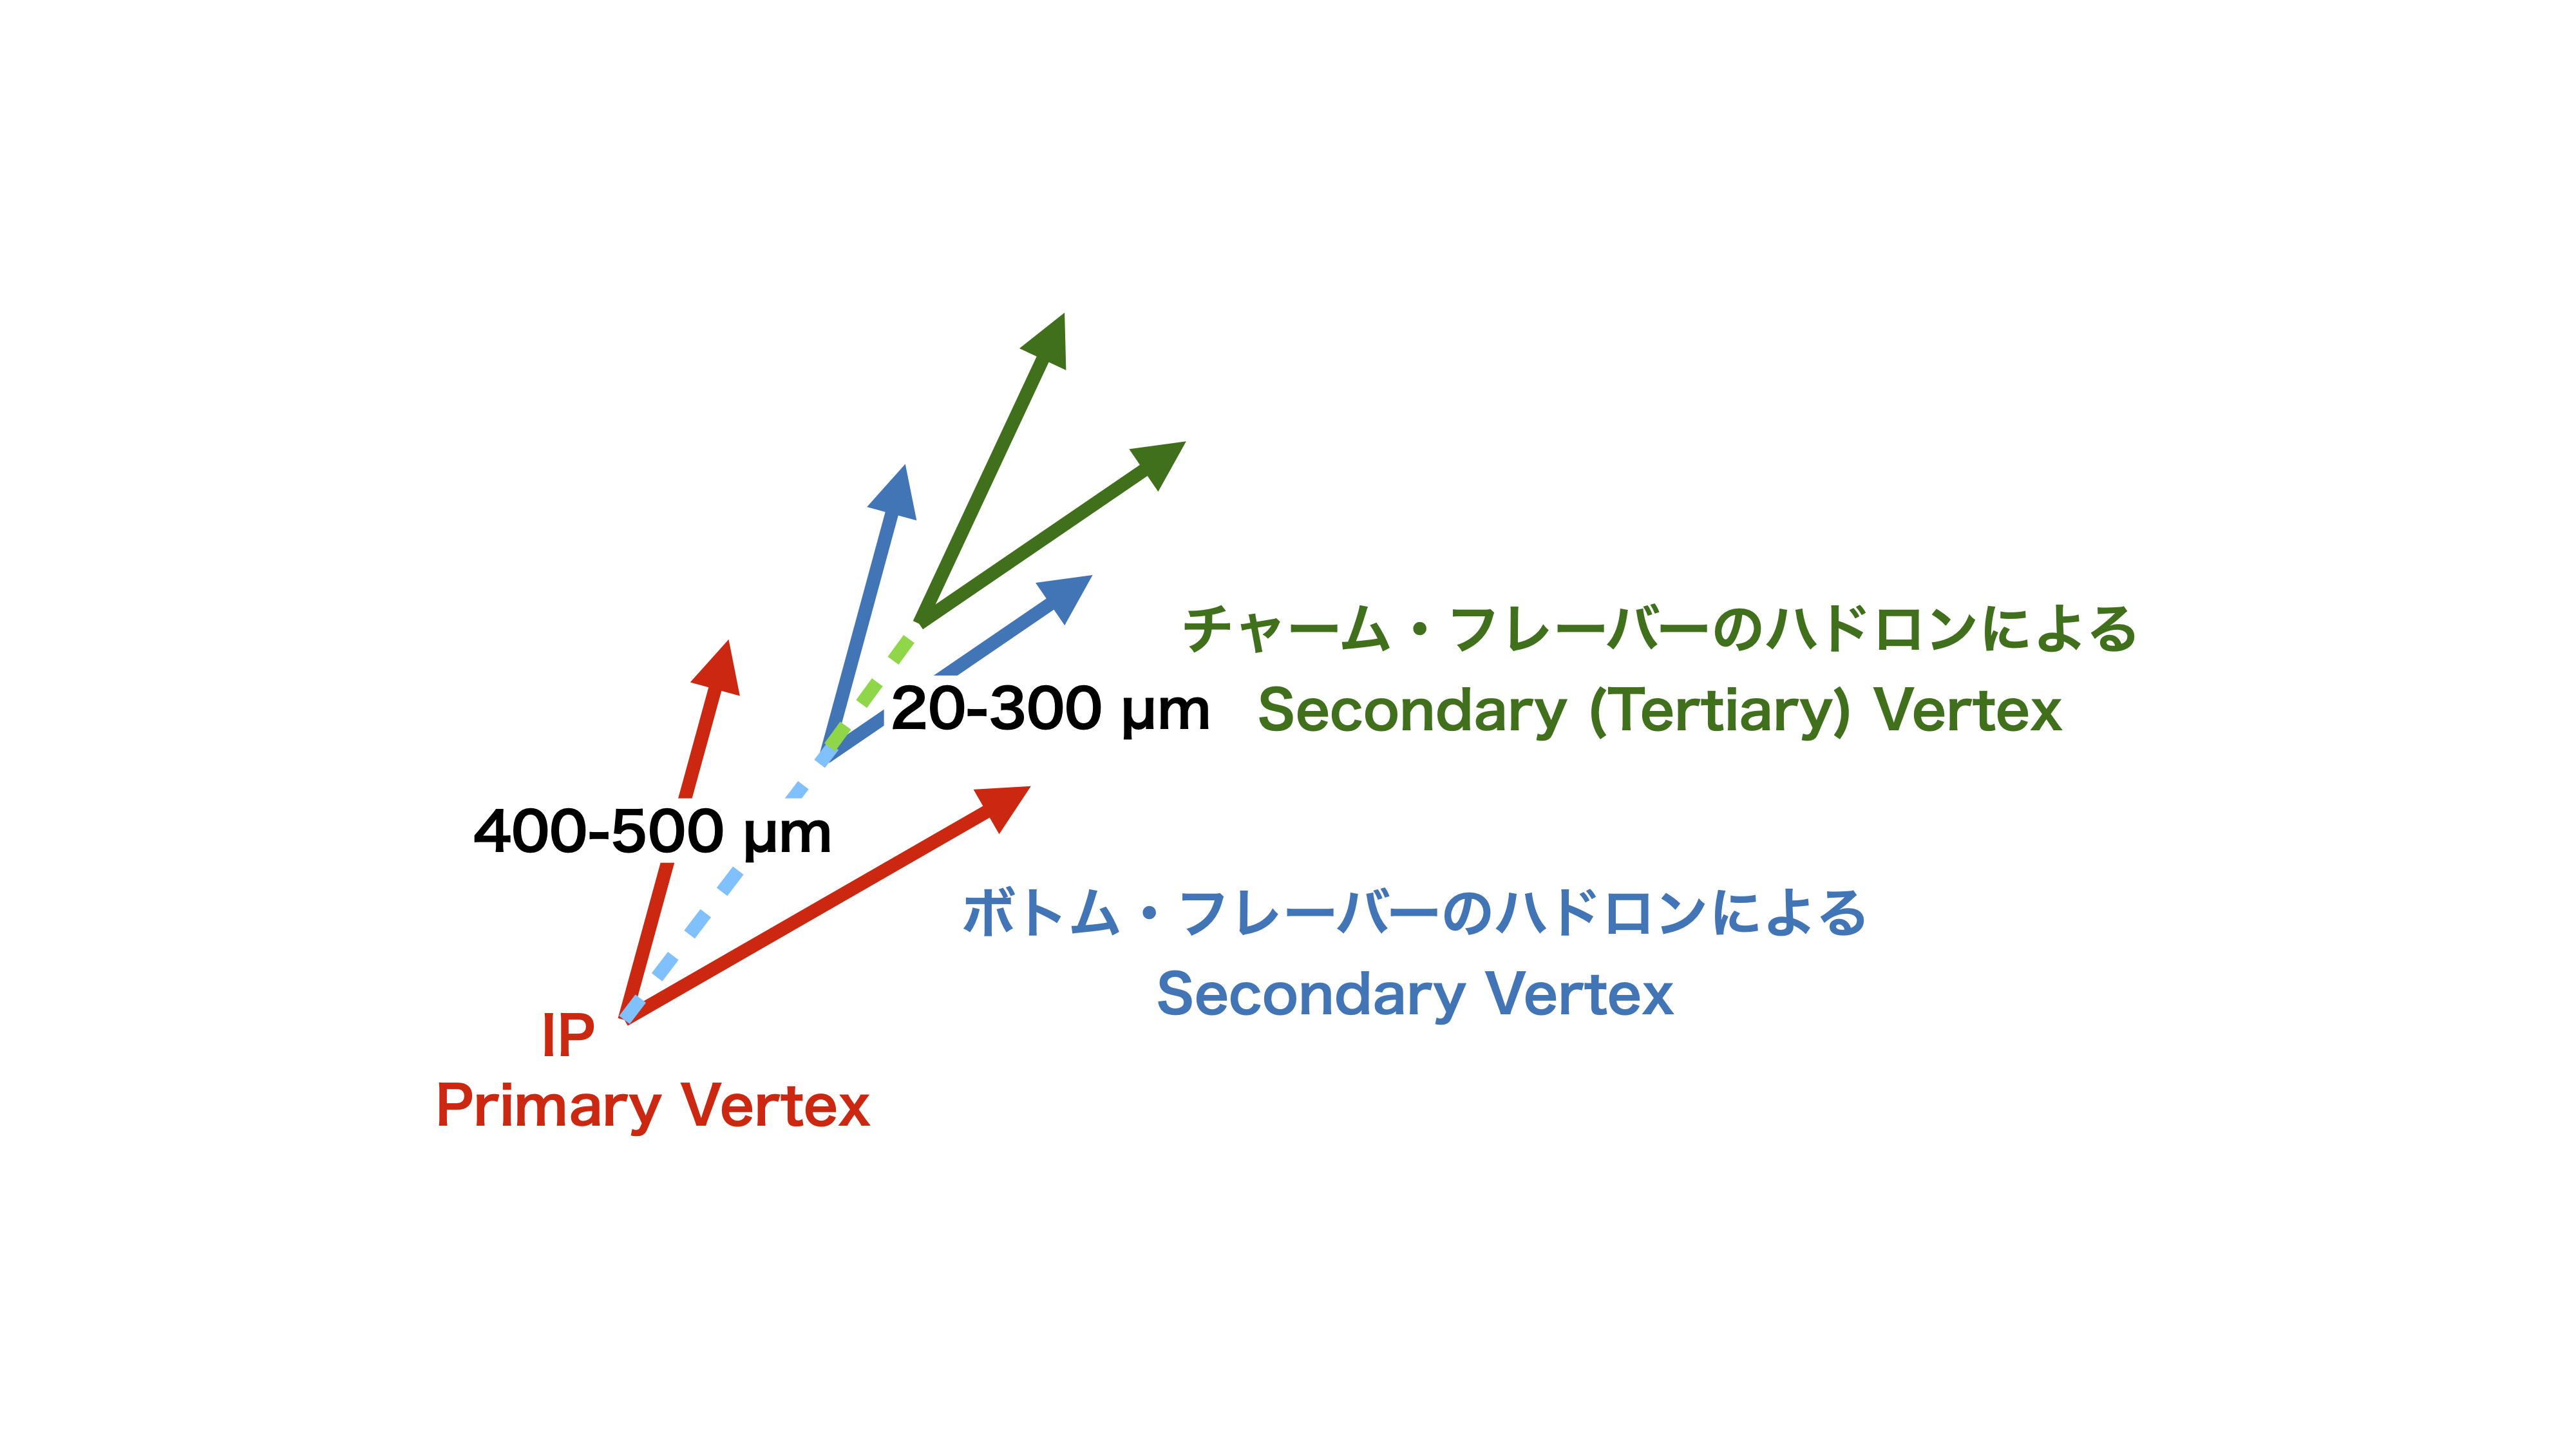
\includegraphics[trim = 0 100 0 50, width=0.9\textwidth]{Figure/3Networks/3-1-1-1FinalStateBB.png}
 \caption{終状態$\rm b\bar{b}$での典型的な崩壊点の例}
 \label{3-1-1-1FinalStateBB}
\end{figure}

図\ref{3-1-1-2TracksandVertices}は1事象に含まれる飛跡の本数と崩壊点の個数である。

\begin{figure}[htbp]
 \centering
 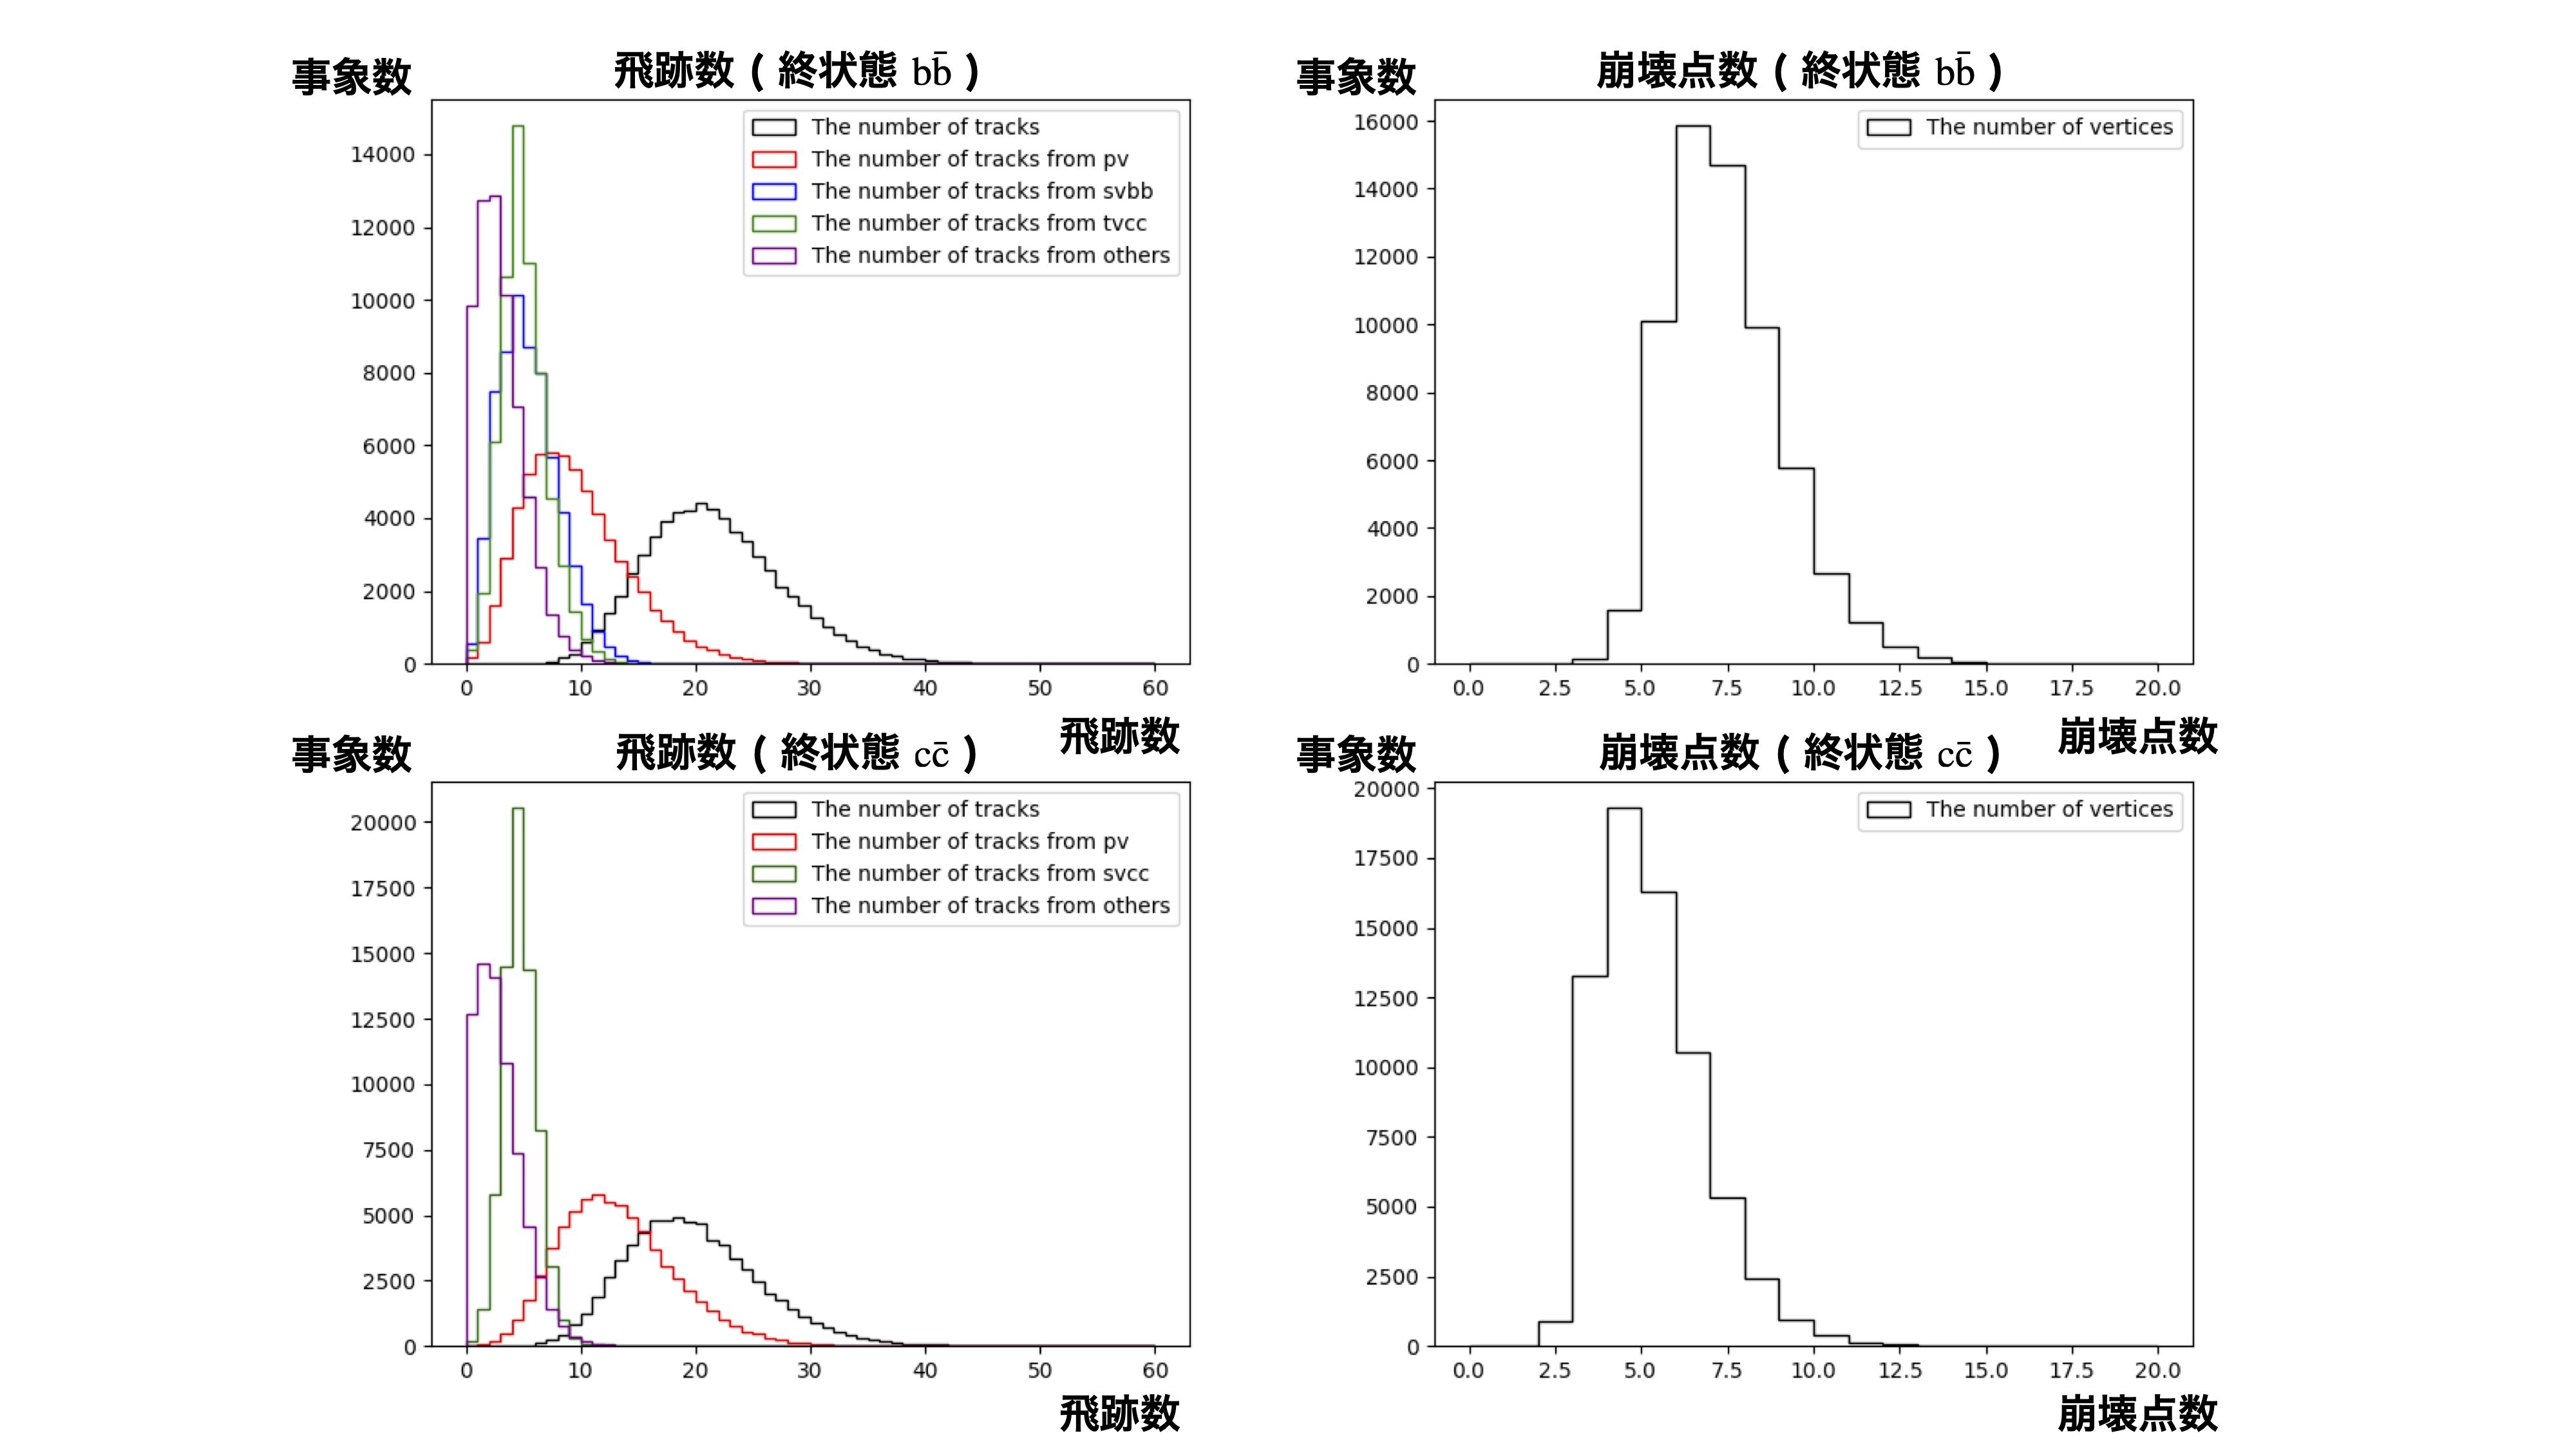
\includegraphics[width=1.0\textwidth]{Figure/3Networks/3-1-1-2TracksandVertices.png}
 \caption{事象に含まれる飛跡の本数と崩壊点の個数}
 \label{3-1-1-2TracksandVertices}
\end{figure}


(未完)

%%%%%%%%%%%%%%%%%%%%%%%%%%%%%%%%%%%%%%%%%%%%%%%%%%%%%%%%%%%%%%%%%%%%%%%%
\subsection{飛跡の情報と前処理} \label{Net:Data:TrackInformationandPreprocessing}

本研究では、崩壊点を探索するにあたって飛跡の情報として、図\ref{3-1-1-2TrackParameters}のような位置や運動量を含んだトラック・パラメータ($\rm d_0$, $\rm z_0$, $\rm \phi$, $\rm \Omega$, $\rm \tan{\lambda}$)\cite{TrackParametersLCIO}とその共分散行列、電荷、エネルギーの$22$個の変数を使用した。

\begin{figure}[htbp]
 \centering
 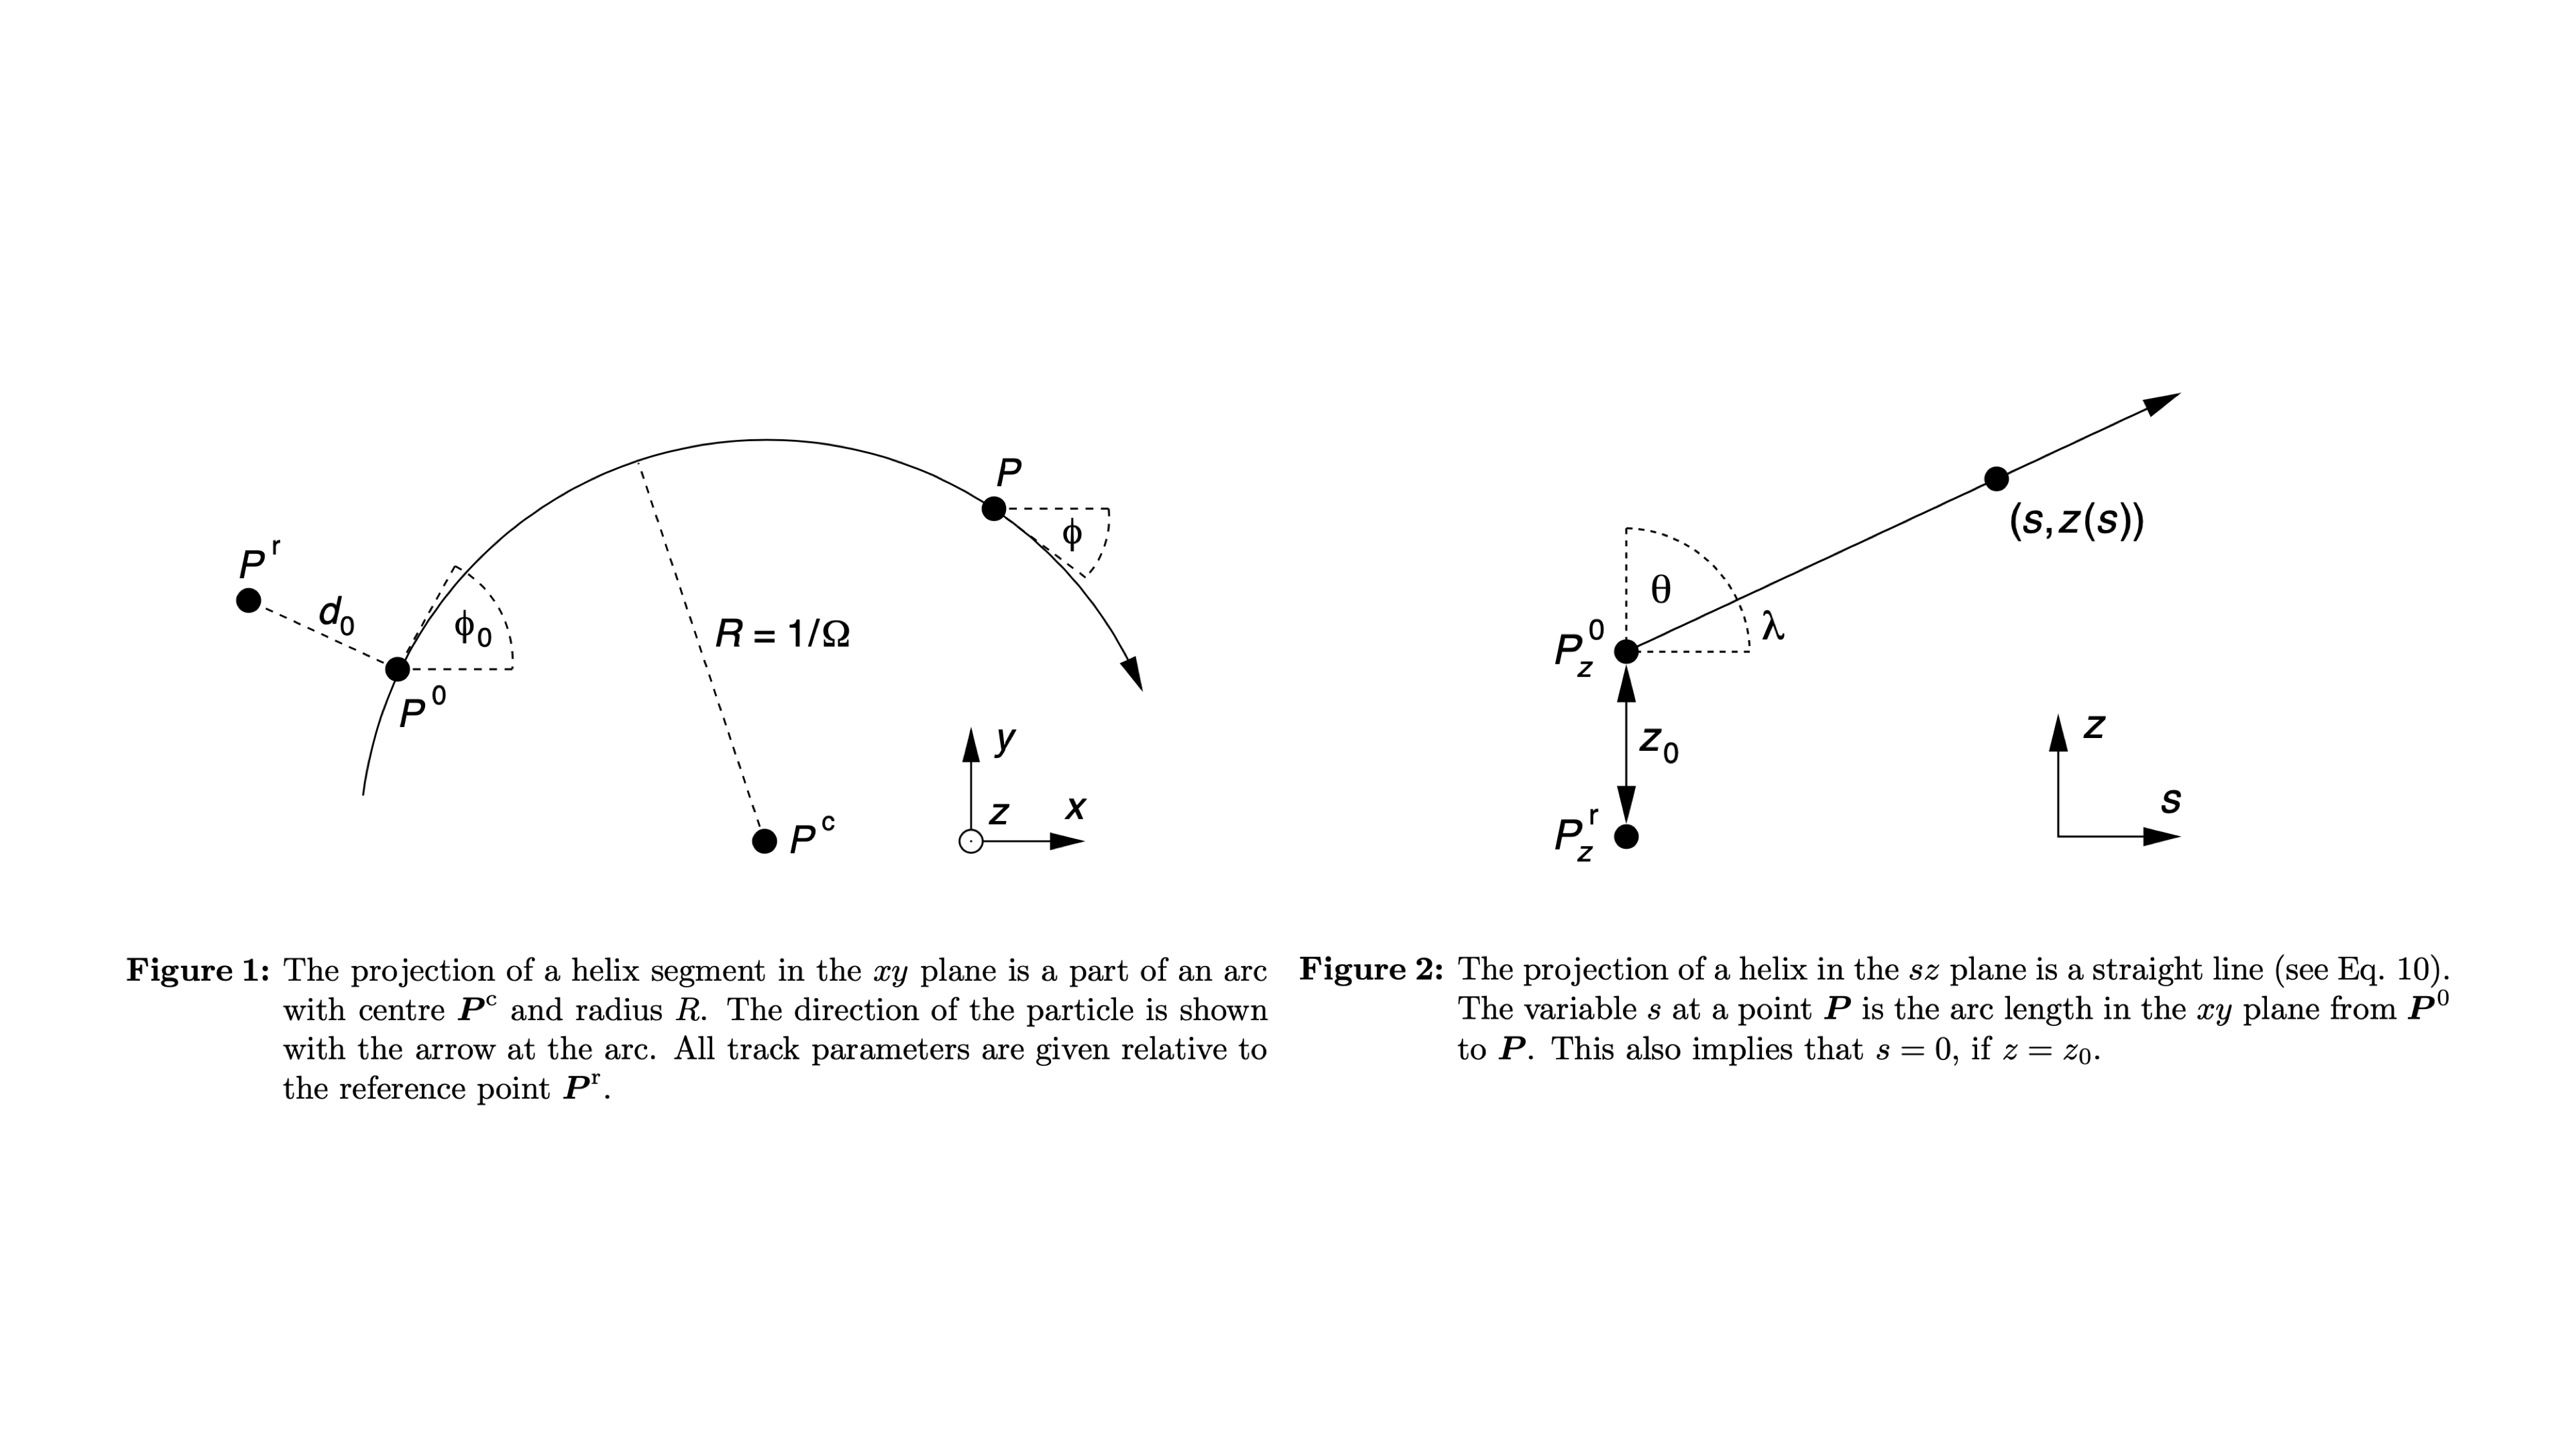
\includegraphics[trim = 0 150 0 150, width=1.0\textwidth]{Figure/3Networks/3-1-2-1TrackParameters.png}
 \caption{トラック・パラメータ\cite{TrackParametersLCIO}}
 \label{3-1-2-1TrackParameters}
\end{figure}

深層学習の入力として扱う場合は、一般に$[-1,\ 1]$の範囲に変数を整形した方が良いと言われている。
したがって、それぞれの変数を以下のような$\tanh$関数や線形関数などを用いて変換した。

\begin{itemize}
 \item トラック・パラメータ\\
 ${\rm d_0} = \tanh{({\rm d_0})}$,
 ${\rm z_0} = \tanh{({\rm z_0})}$,
 ${\rm \phi} = {\rm \phi}/\pi$,
 ${\rm \Omega} = \tanh{(200{\rm \Omega})}$,
 ${\rm \tan{\lambda}} = \tanh{(0.3{\rm \tan{\lambda}})}$
 \item トラック・パラメータの共分散行列 : $\tanh{(8000({\rm x}-0.0005))}$
 \item 電荷 : 変換なし
 \item エネルギー : $\tanh{0.5({\rm x}-5.0)}$
\end{itemize}

トラック・パラメータとエネルギーの変換前の分布と変換後の分布をそれぞれ\ref{3-1-2-2Variables}に示す。

\begin{figure}[htbp]
 \centering
  %\begin{tabular}{cccc}
  \begin{minipage}{1.0\textwidth}
  \centering
   \begin{minipage}{0.48\textwidth}
    \centering
    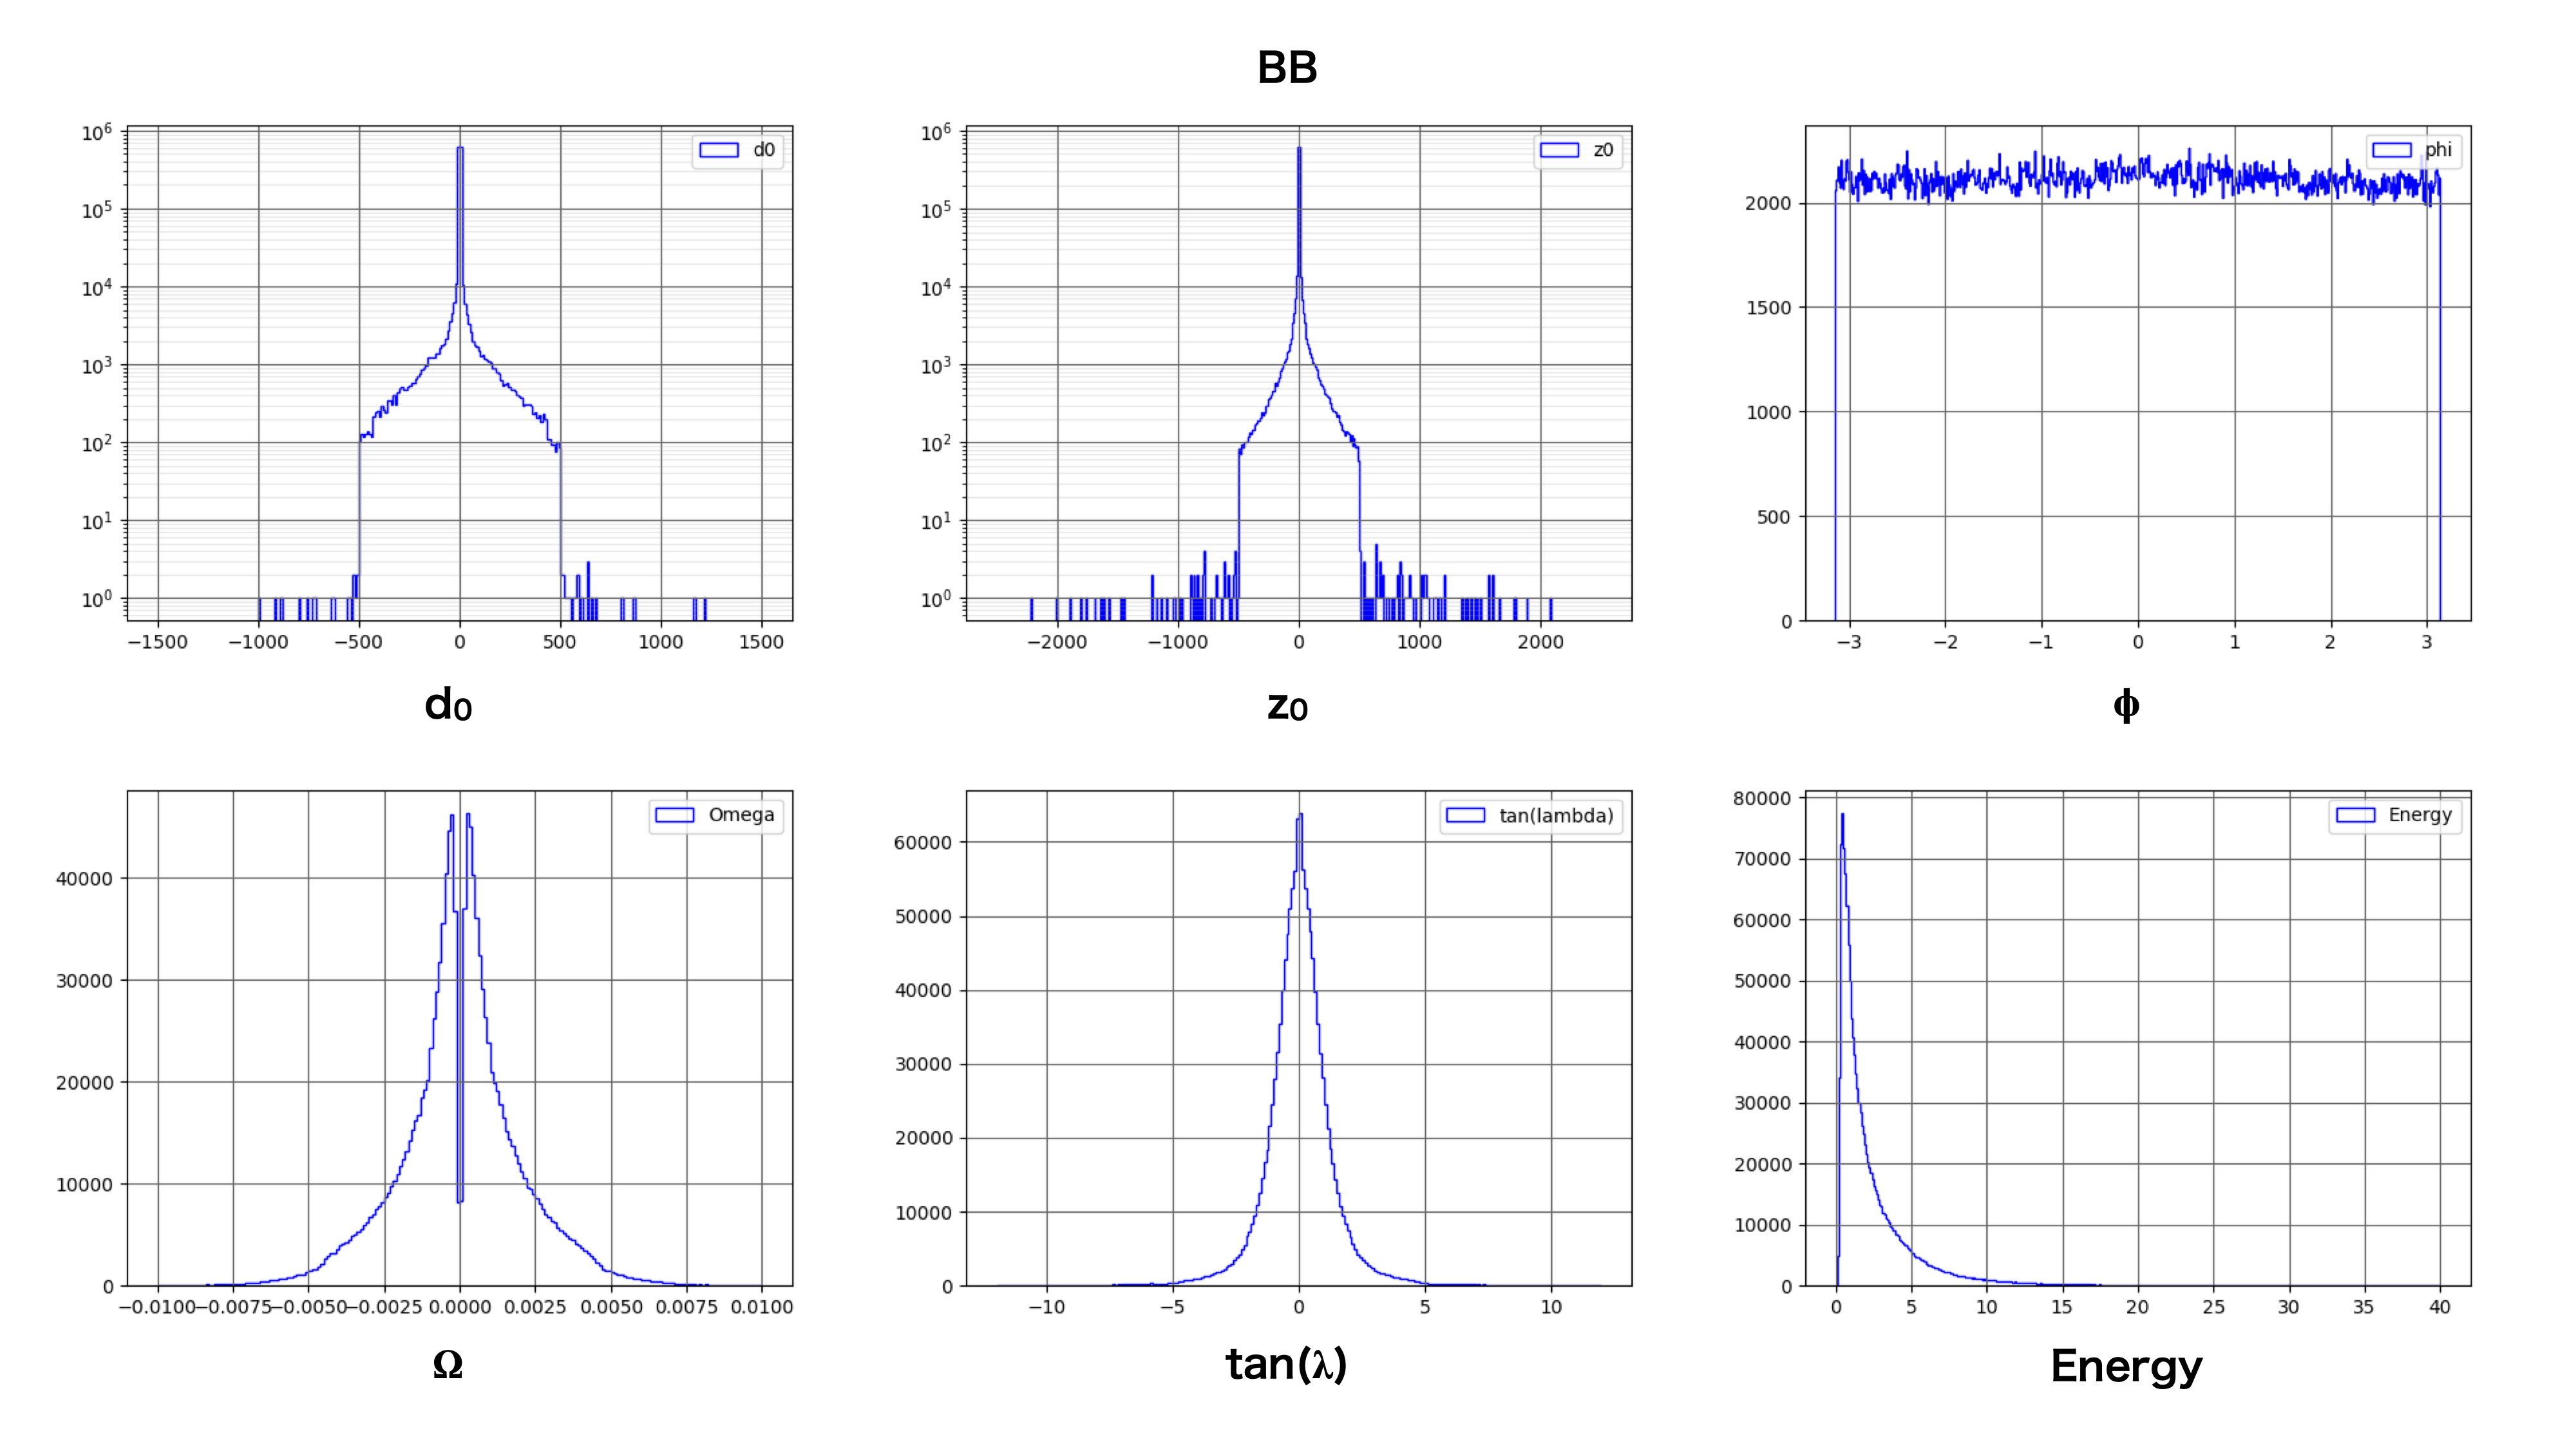
\includegraphics[width=1.0\textwidth, clip]{Figure/3Networks/3-1-2-2OriginalVariablesBB.png}
    \subcaption{終状態$\rm b\bar{b}$での変換前の変数の分布}
    \label{3-1-2-2OriginalVariablesBB}
   \end{minipage}
   \begin{minipage}{0.48\textwidth}
   \centering
    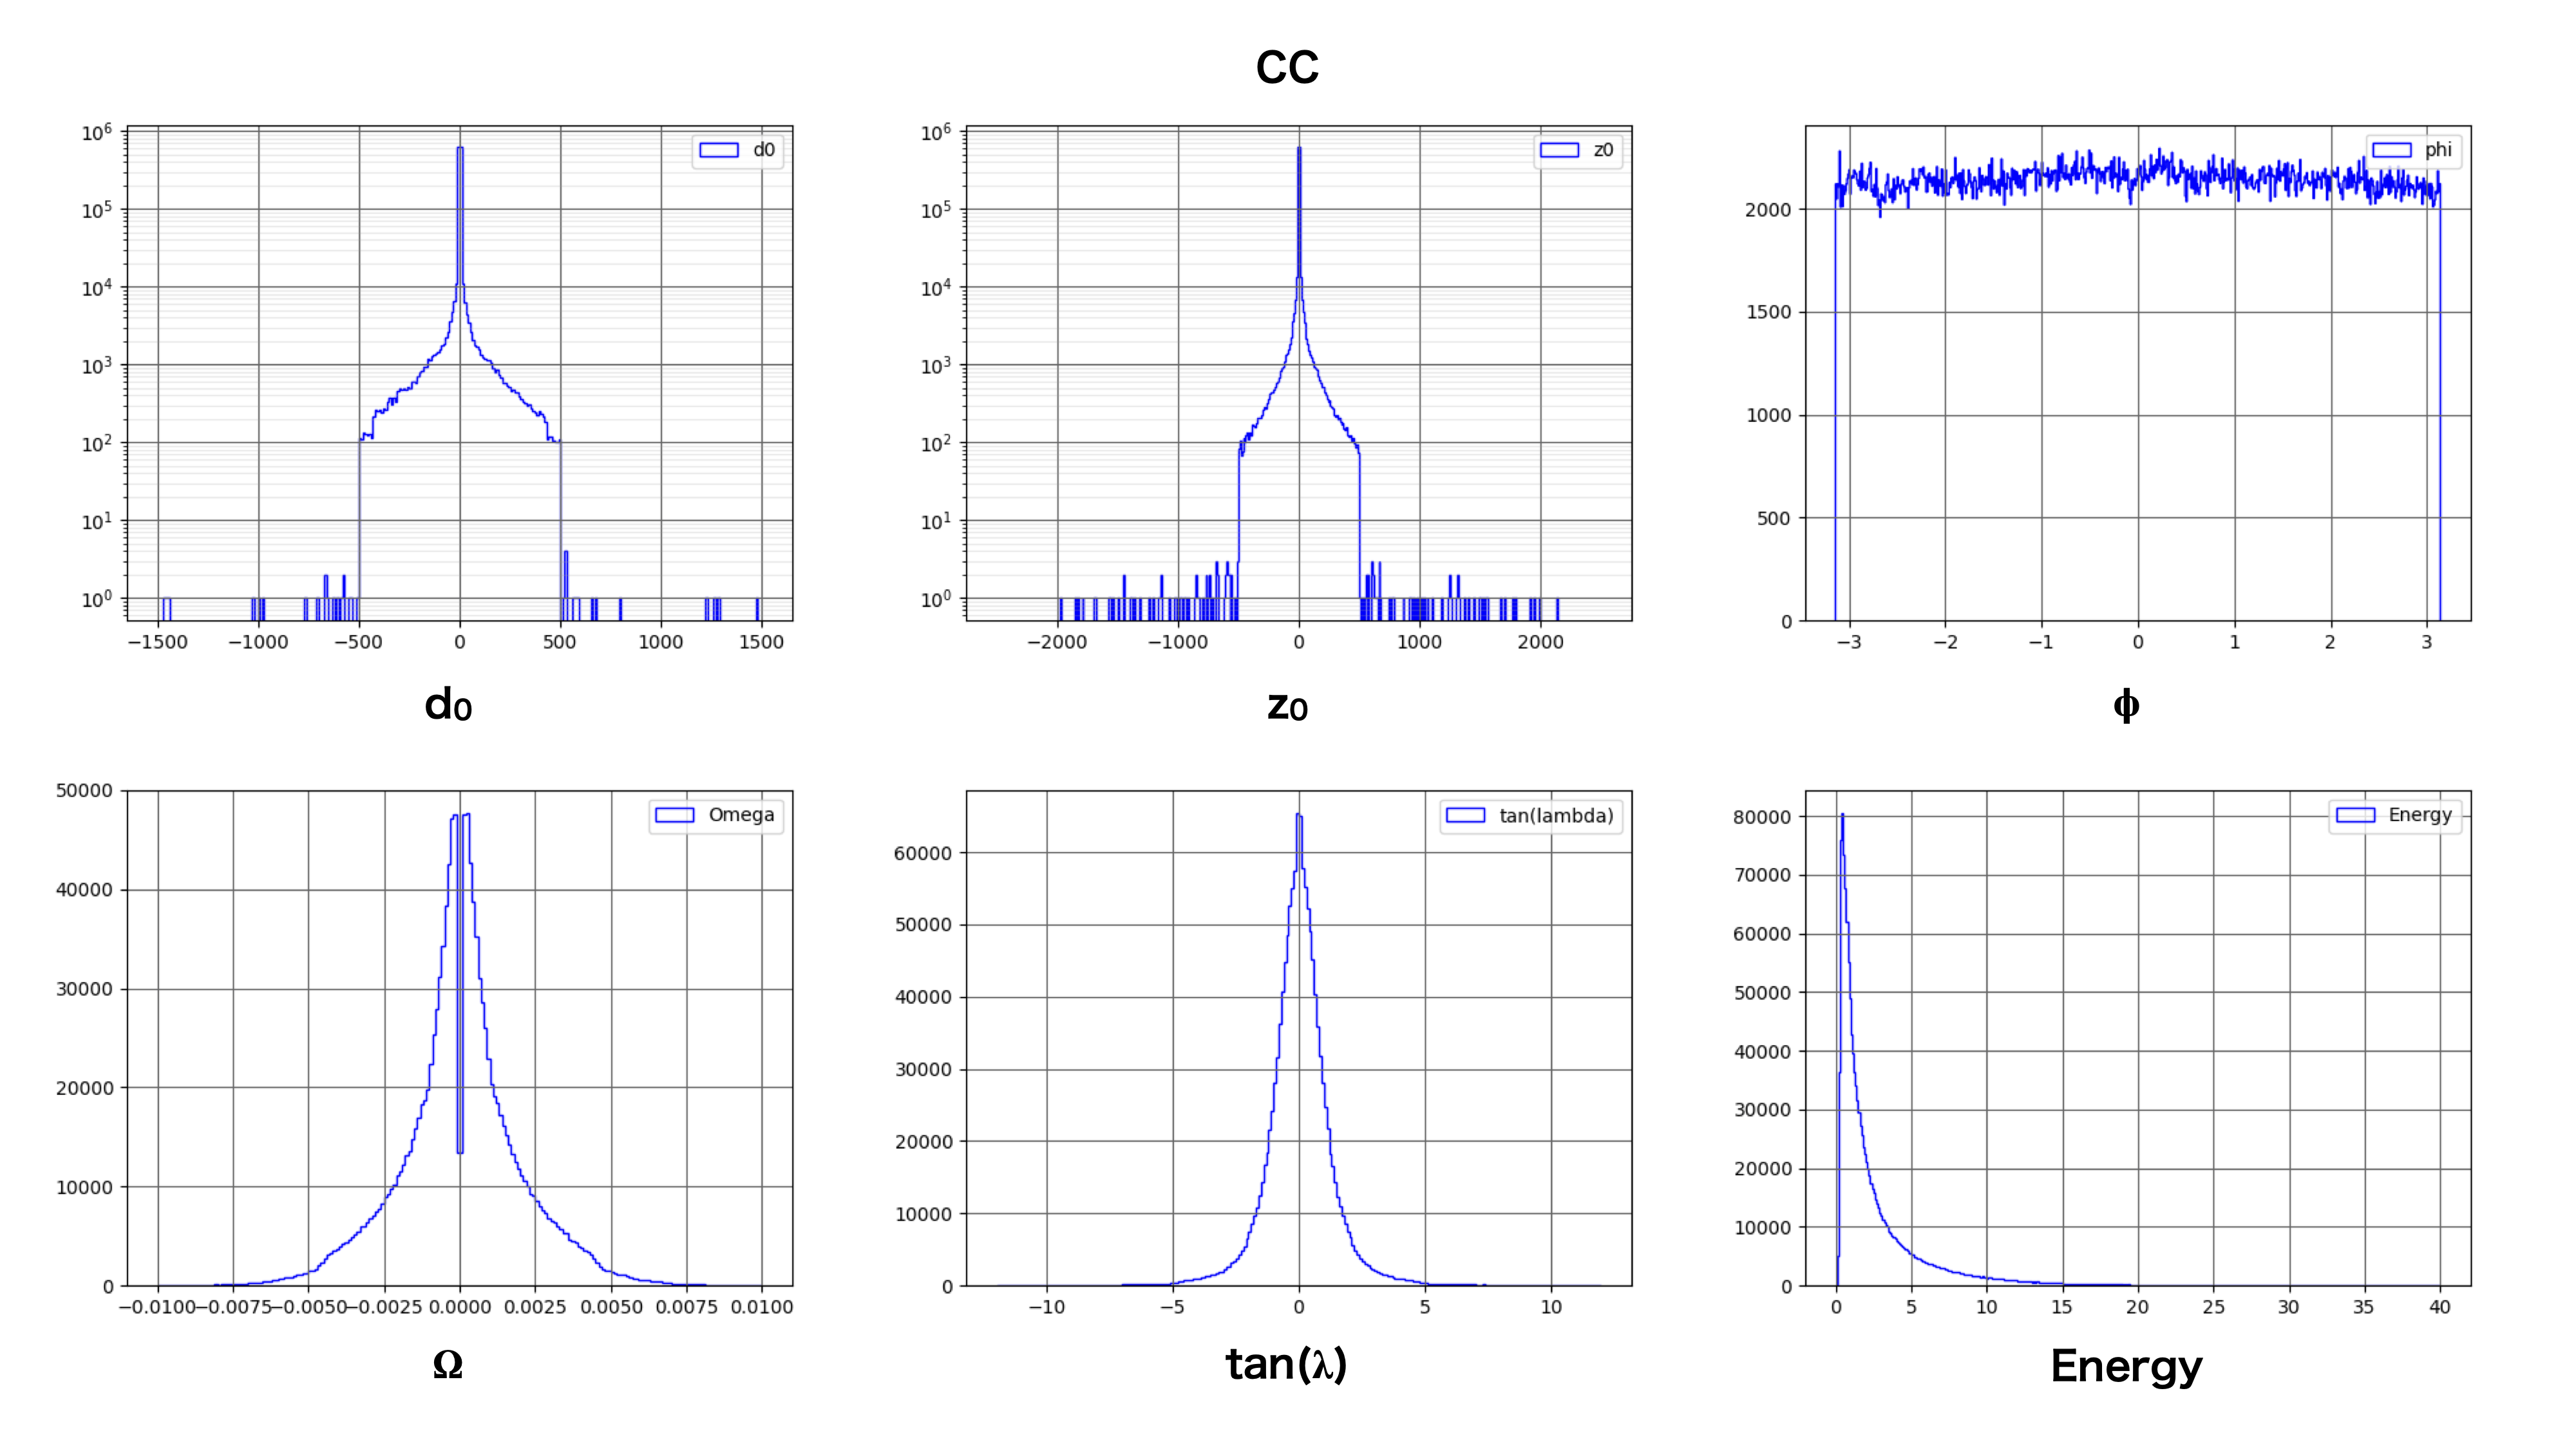
\includegraphics[width=1.0\textwidth, clip]{Figure/3Networks/3-1-2-2OriginalVariablesCC.png}
    \subcaption{終状態$\rm c\bar{c}$での変換前の変数の分布}
    \label{3-1-2-2OriginalVariablesCC}
   \end{minipage}
  \end{minipage}
  
  \begin{minipage}{1.0\textwidth}
  \centering
   \begin{minipage}{0.48\textwidth}
   \centering
    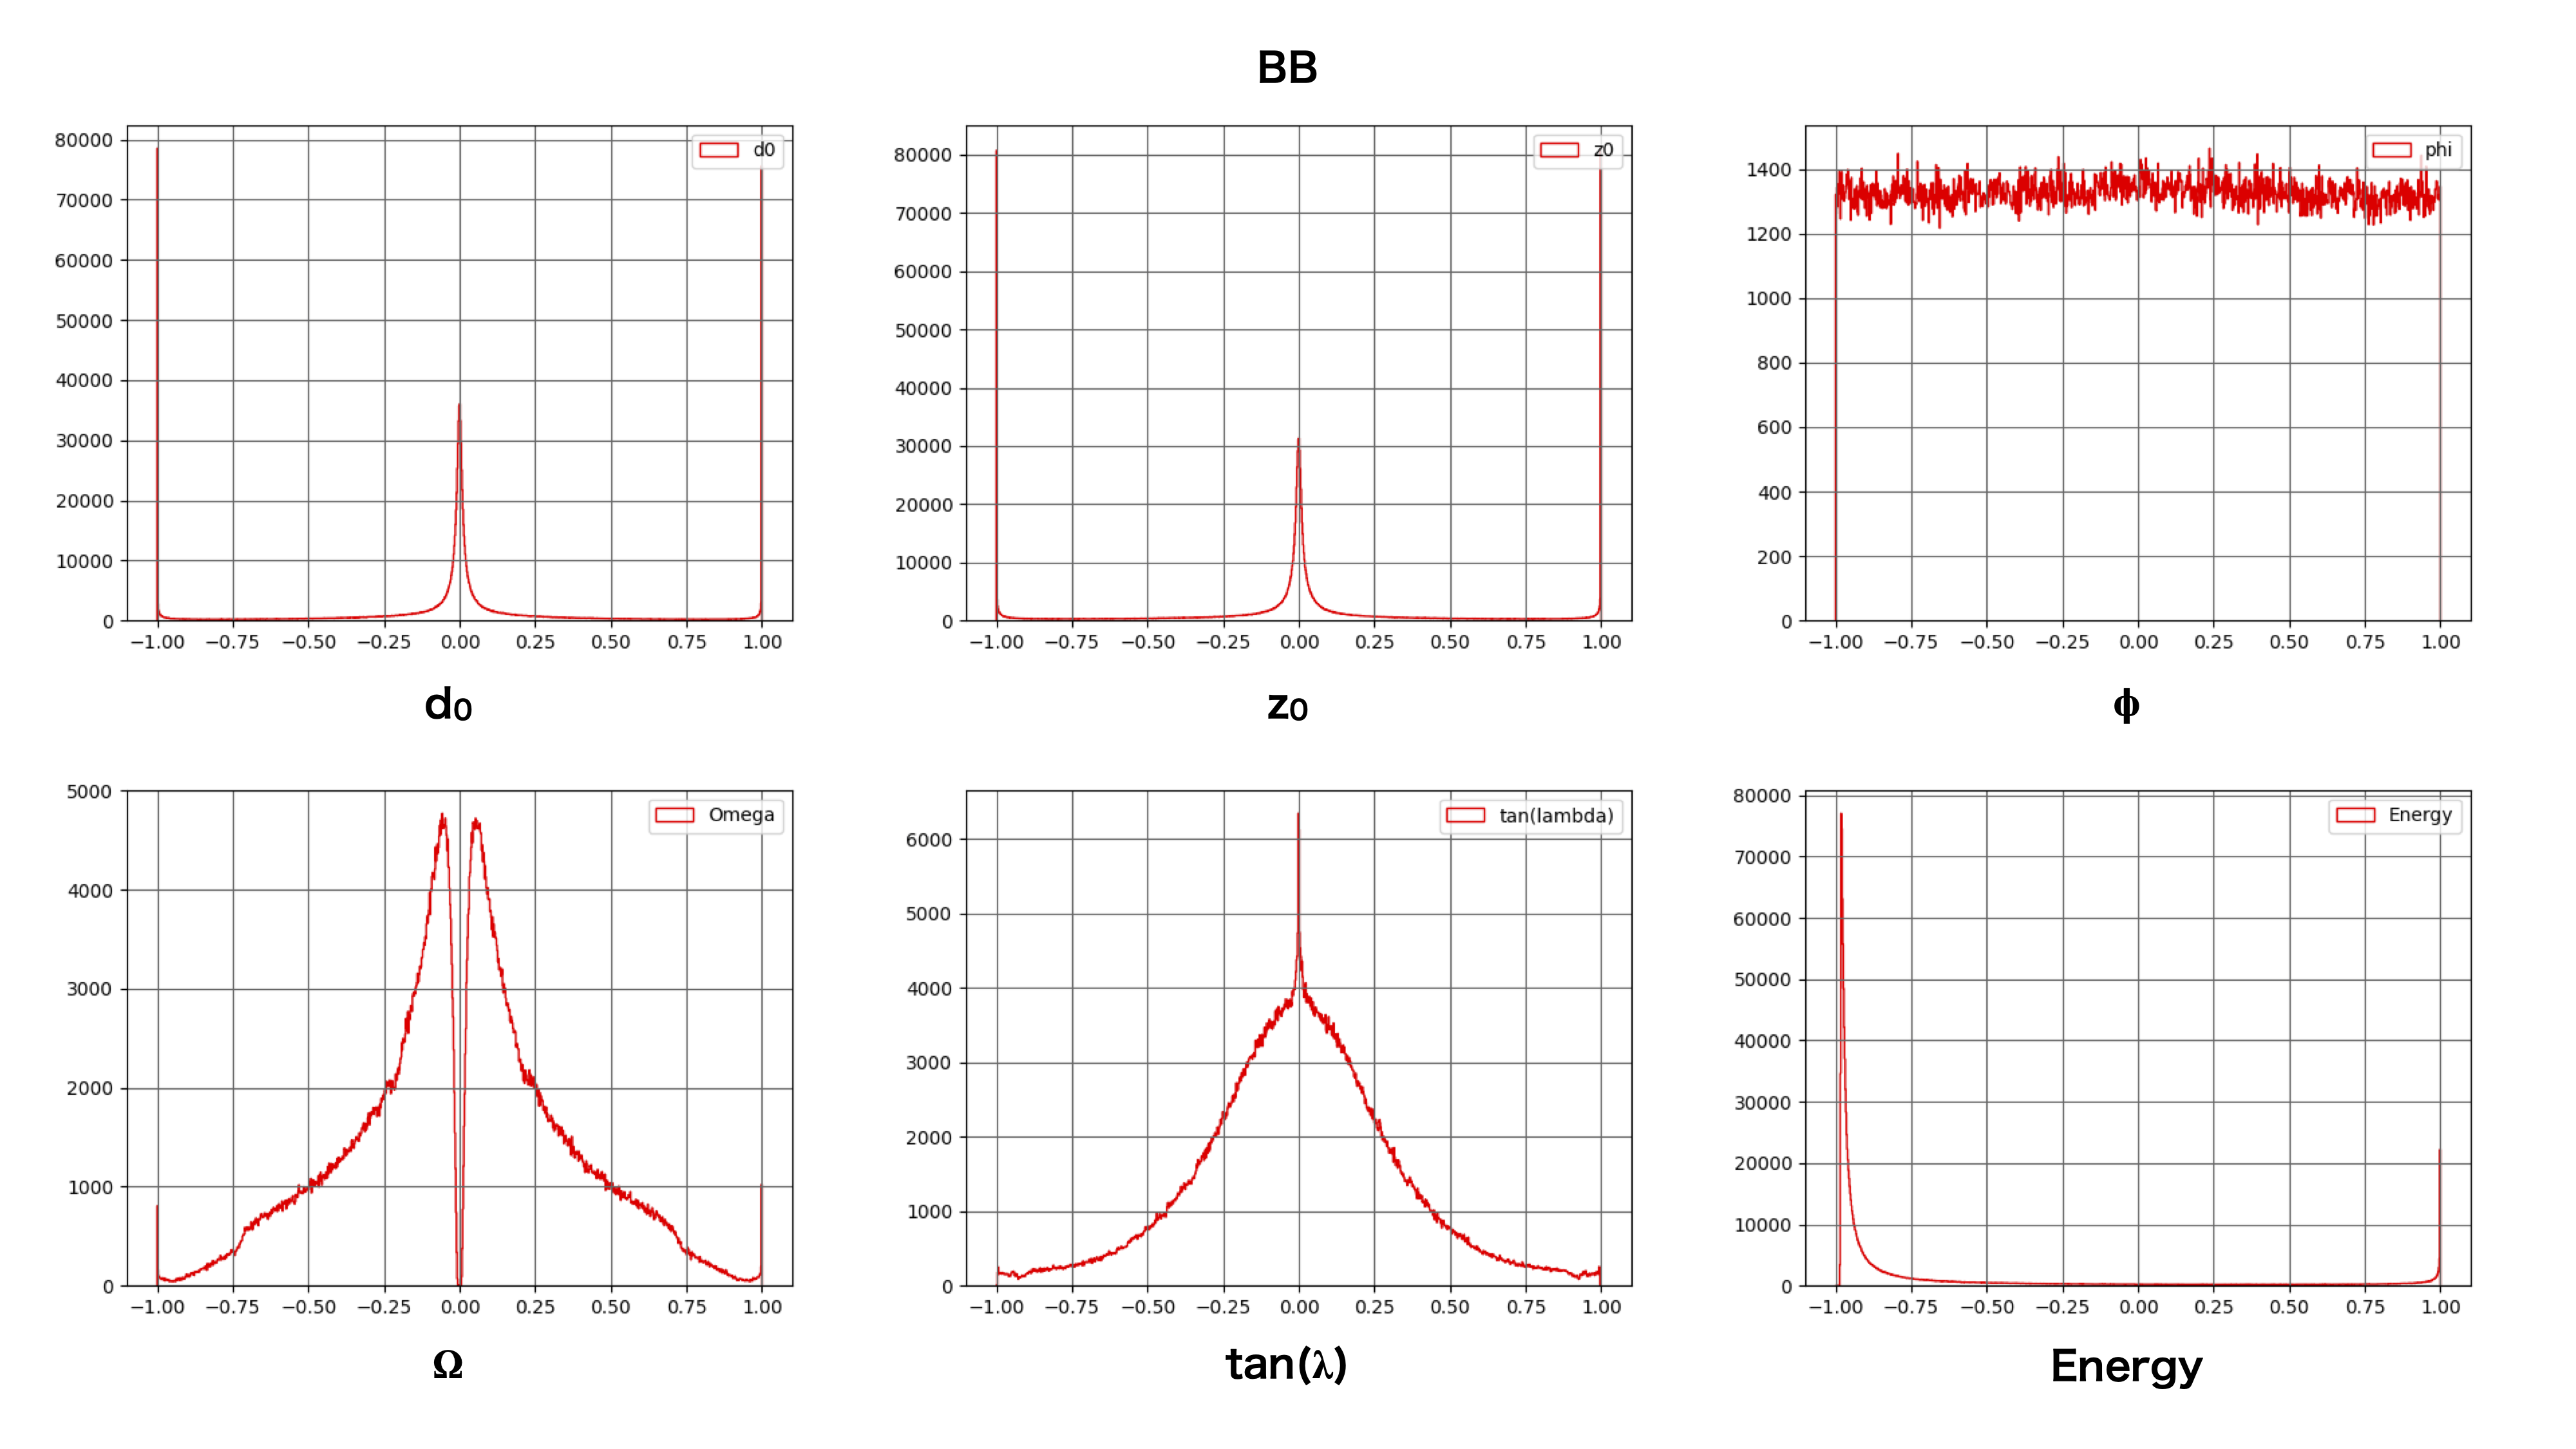
\includegraphics[width=1.0\textwidth, clip]{Figure/3Networks/3-1-2-2ReshapedVariablesBB.png}
    \subcaption{終状態$\rm b\bar{b}$での変換後の変数の分布}
    \label{3-1-2-2ReshapedVariablesBB}
   \end{minipage}
   \begin{minipage}{0.48\textwidth}
   \centering
    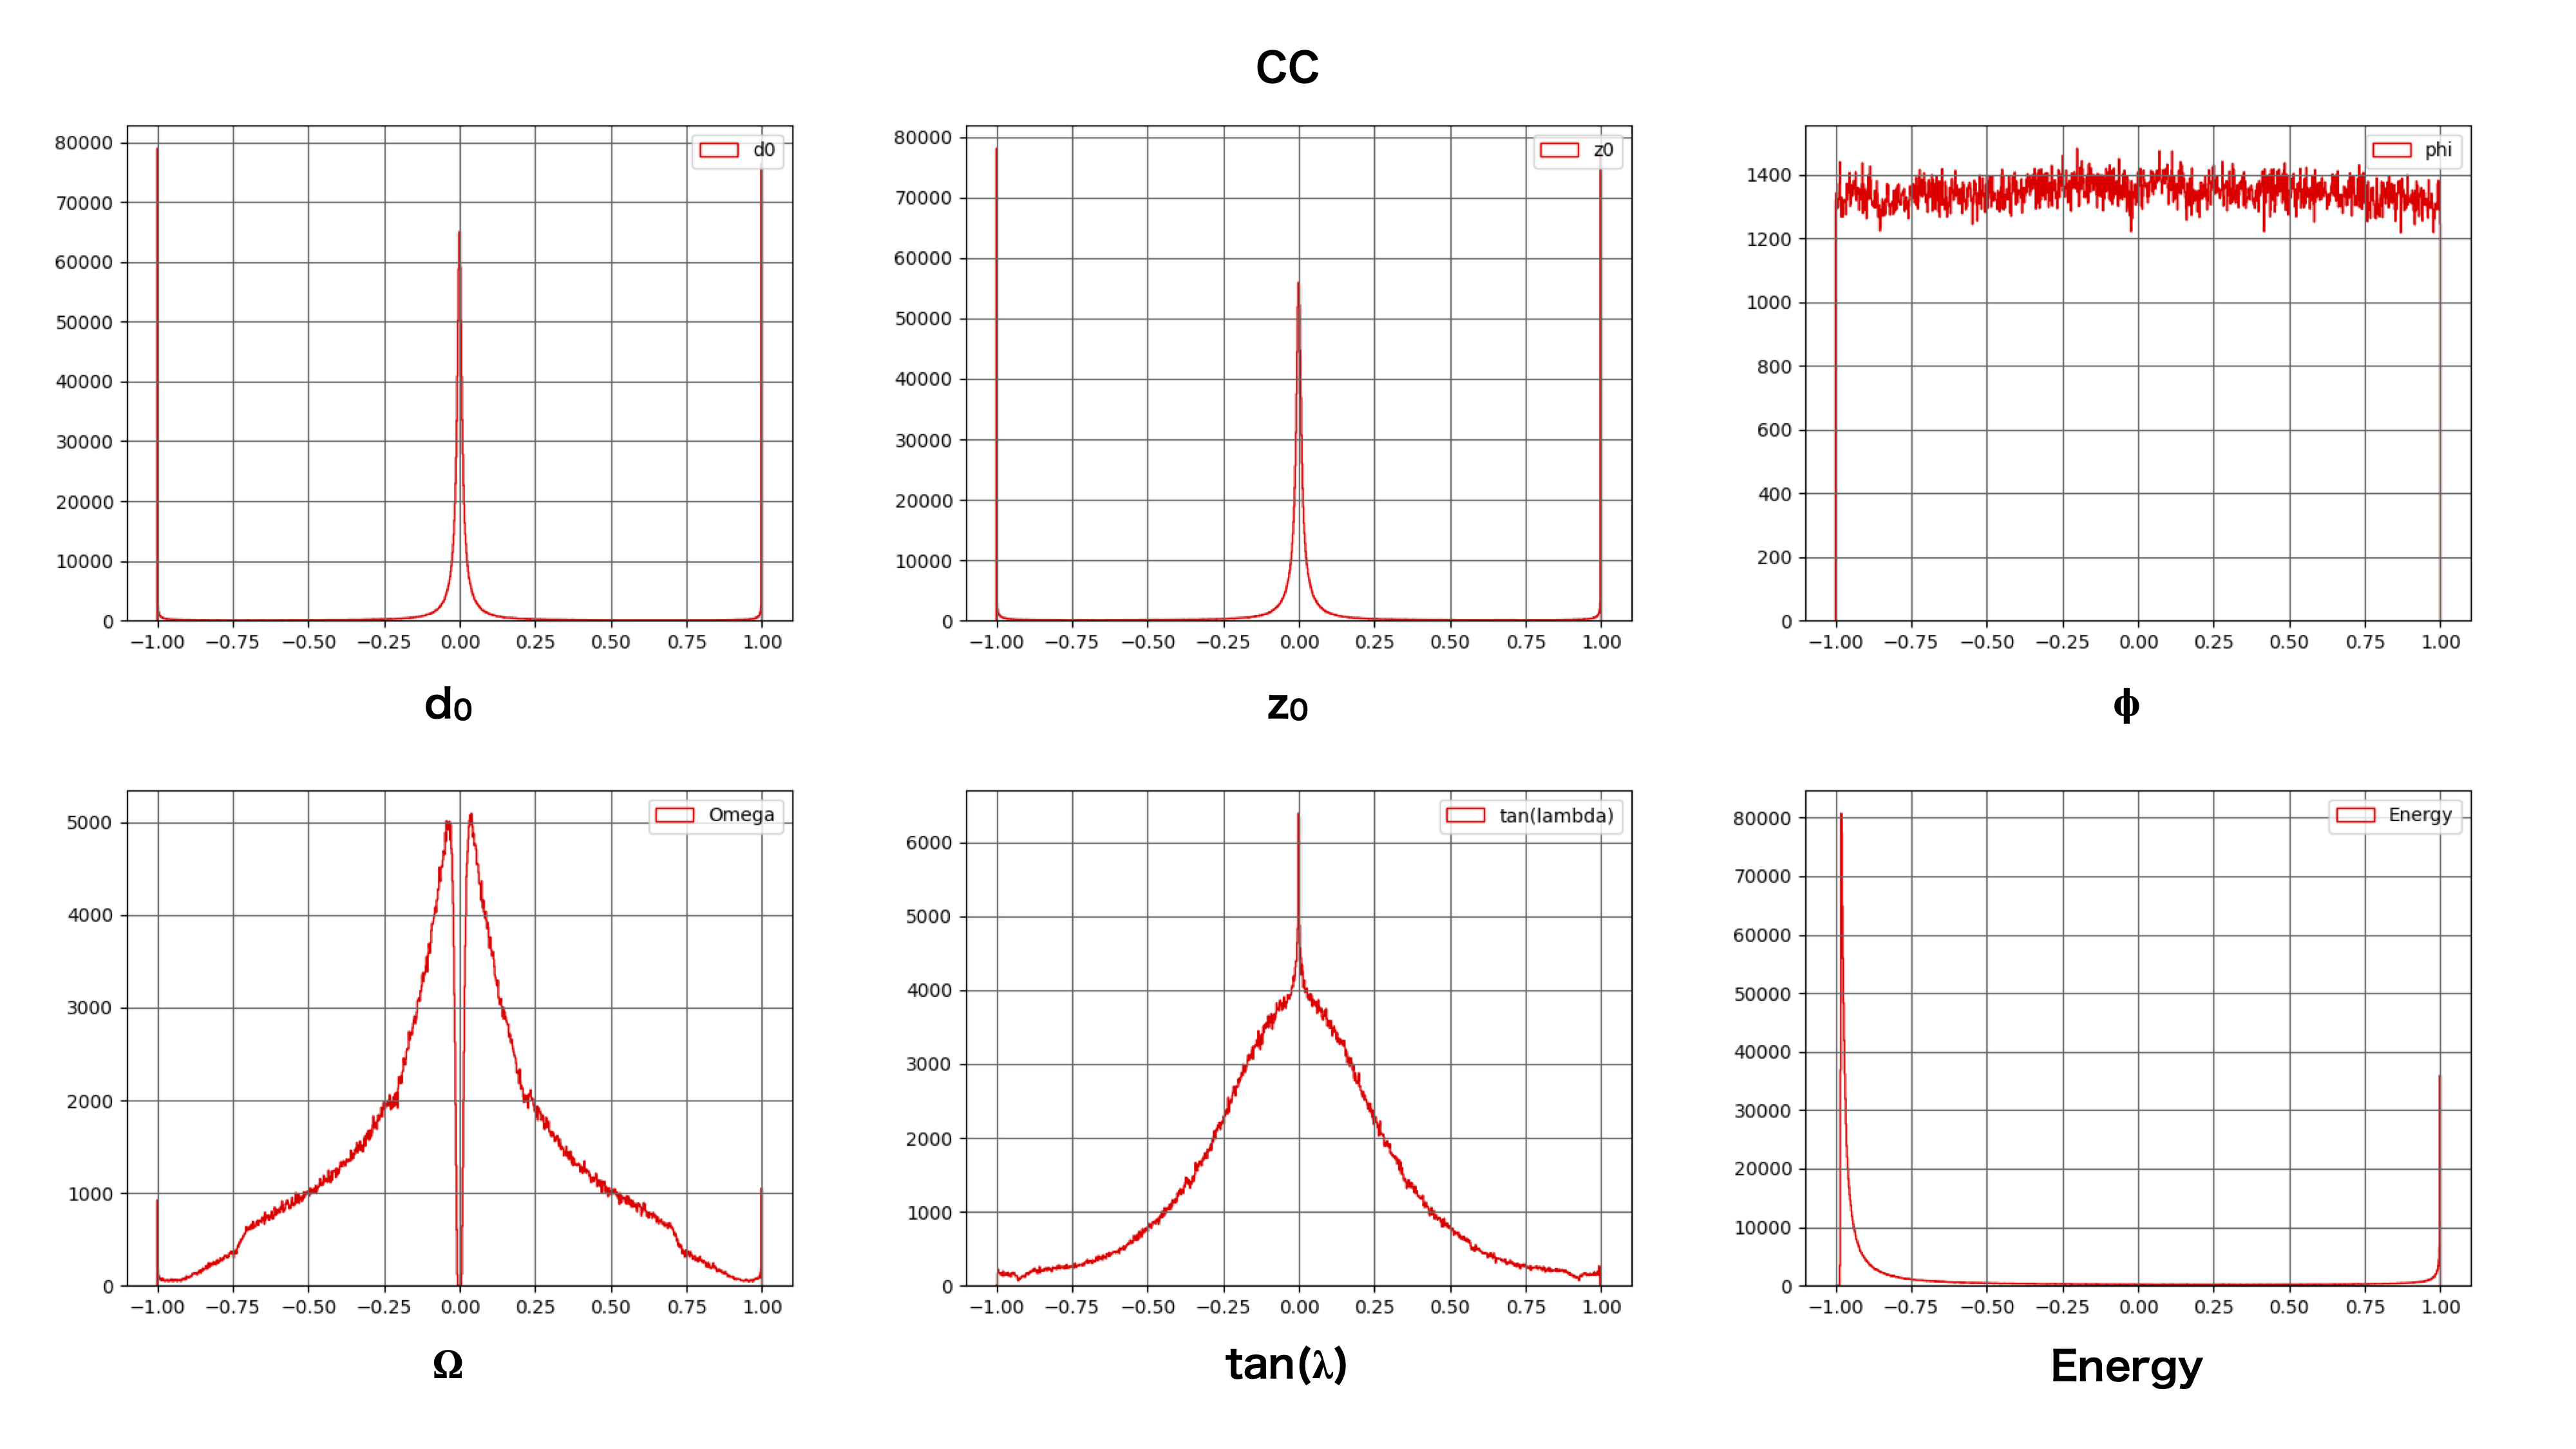
\includegraphics[width=1.0\textwidth, clip]{Figure/3Networks/3-1-2-2ReshapedVariablesCC.png}
    \subcaption{終状態$\rm c\bar{c}$での変換後の変数の分布}
    \label{3-1-2-2ReshapedVariablesCC}
   \end{minipage}
   \end{minipage}
  \caption{変数の分布の例}
  \label{3-1-2-2Variables}
 %\end{tabular}
\end{figure}

また、LCFIPlusのフィッティングで得られる変数であるカイ二乗や予想される崩壊点の位置についてもデータを用意した。
これらの値は1事象中の任意の二本の飛跡 (飛跡対) について計算を行ったものである。
ただし、深層学習の学習においてはこの値は基本的には使用せず、学習の健全性を確かめる目的や正解ラベルとして用いこととする。
LCFIPlusによって予想される崩壊点の位置の分布を図\ref{}に示す。

\begin{figure}[htbp]
 \centering
 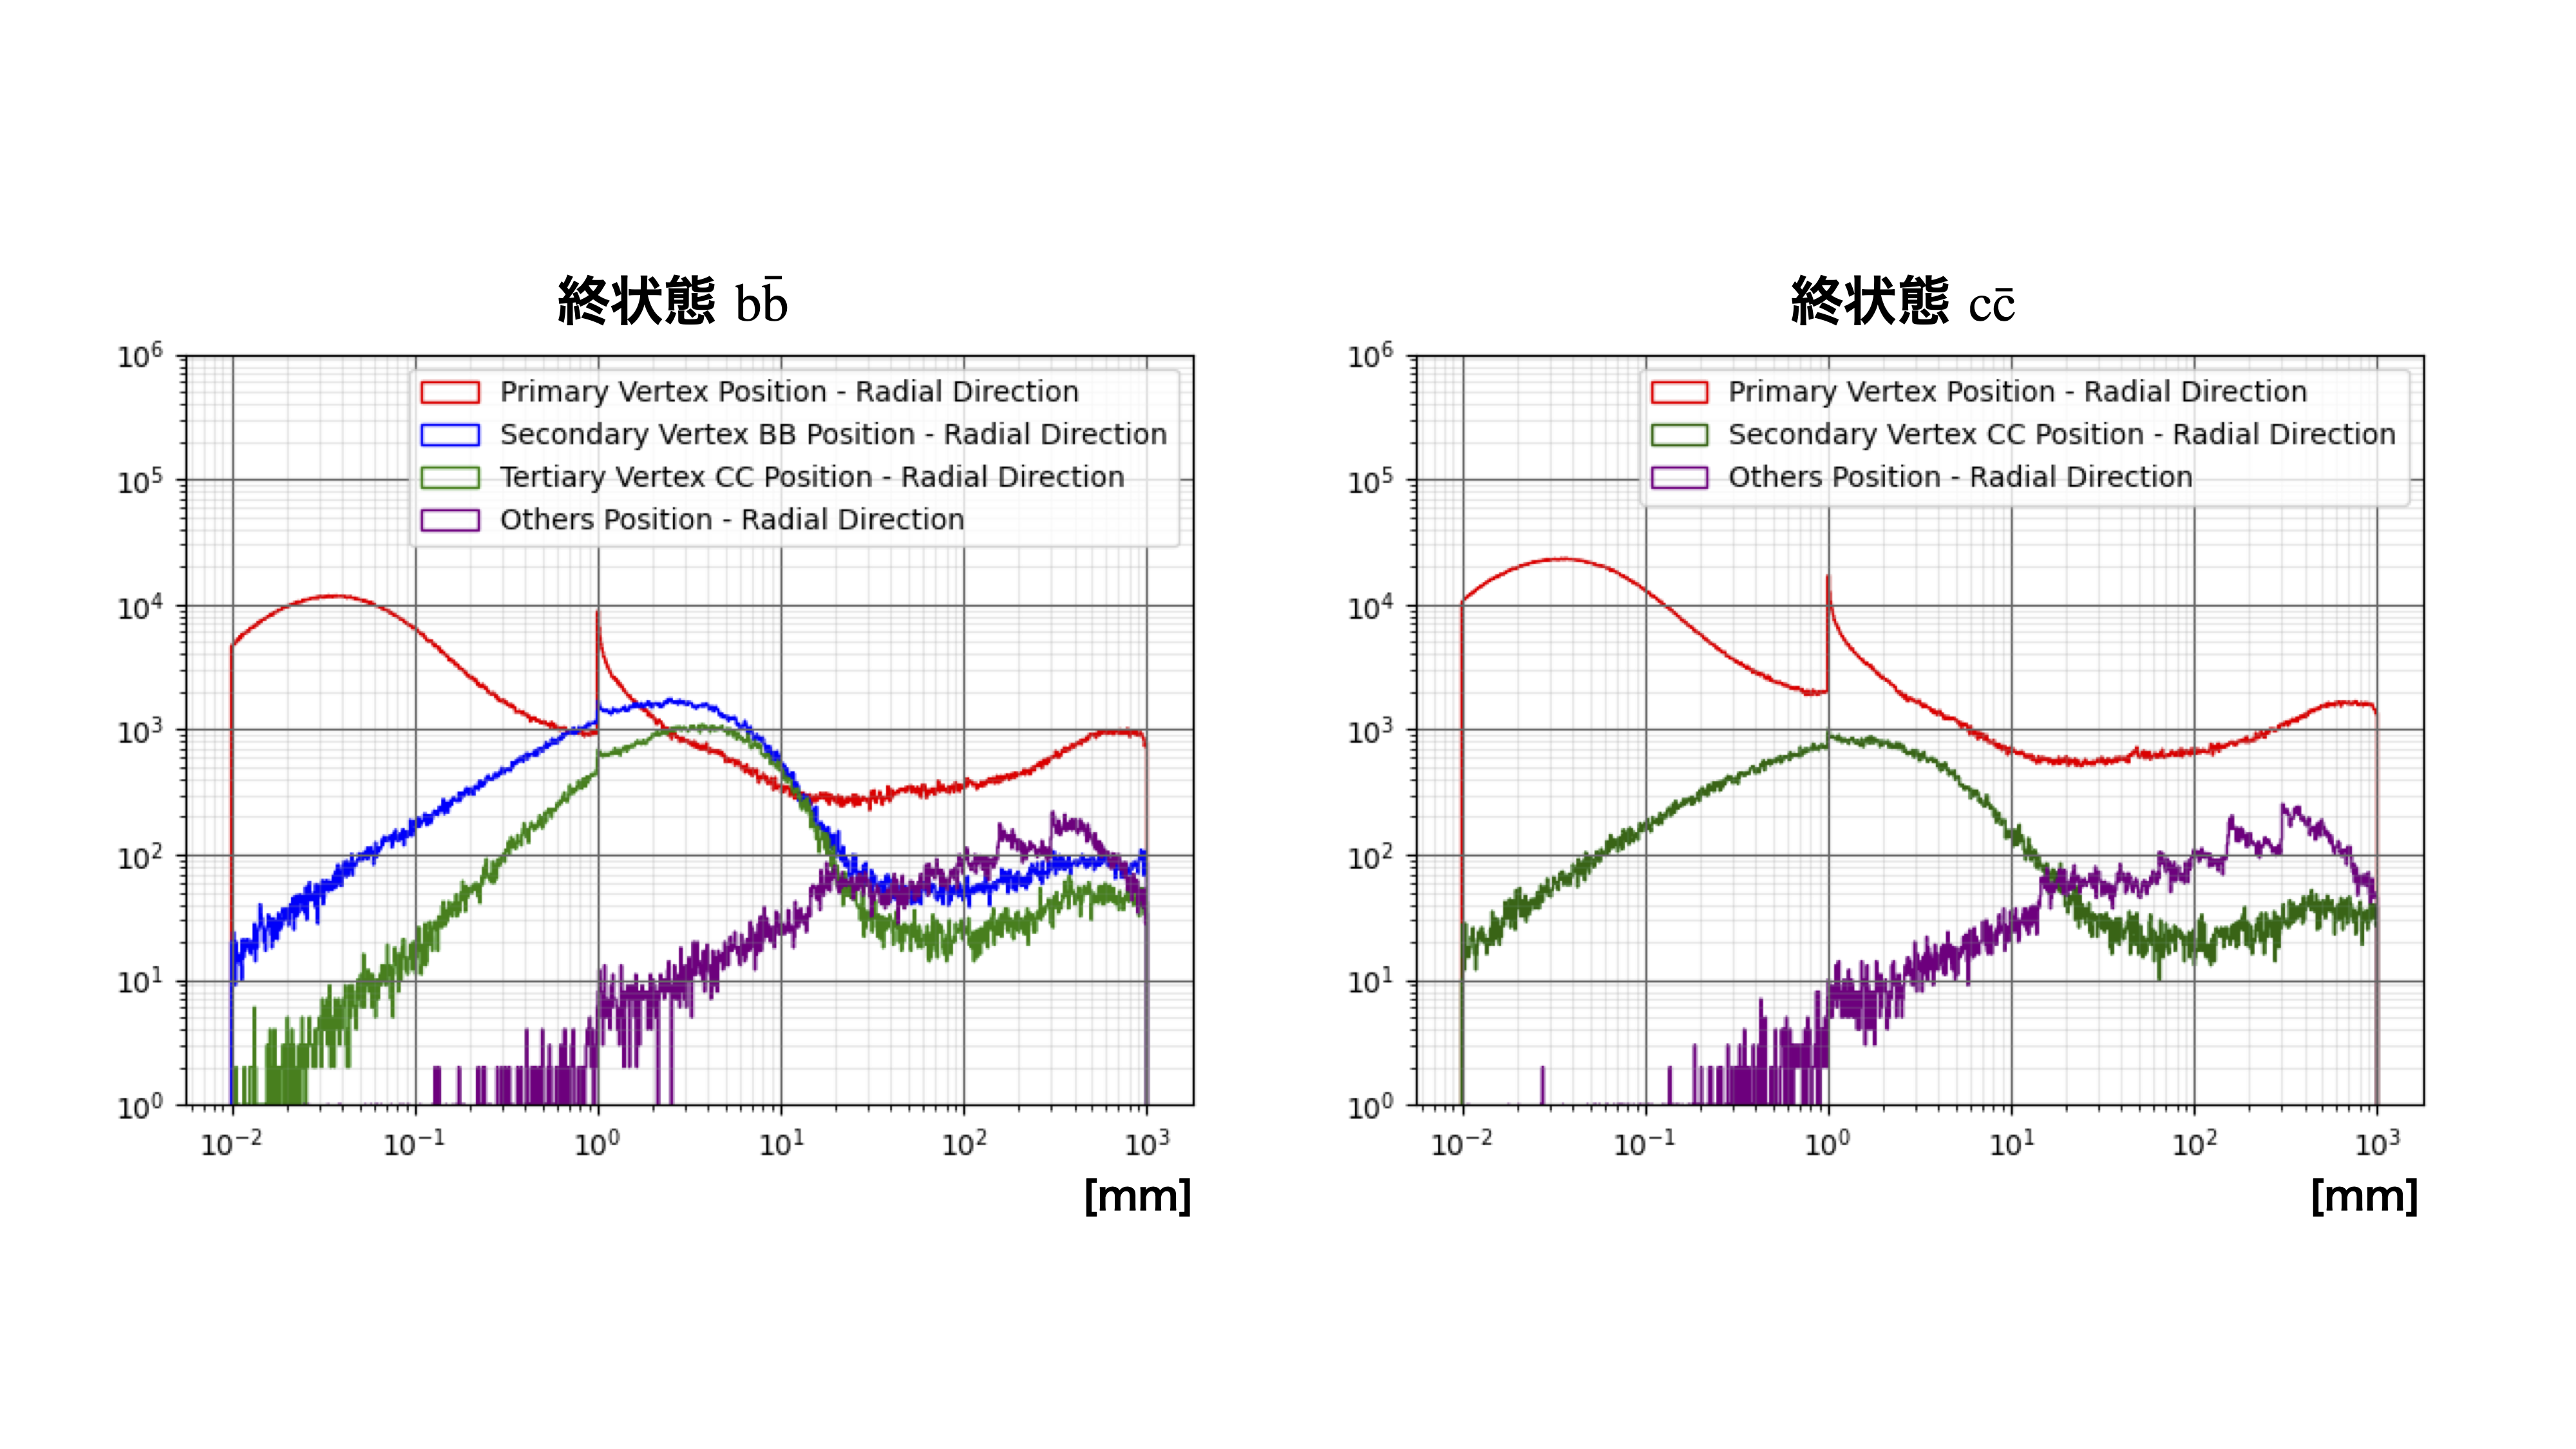
\includegraphics[width=1.0\textwidth]{Figure/3Networks/3-1-2-3VertexPositions.png}
 \caption{LCFIPlusによって予想される崩壊点の位置の分布}
 \label{3-1-2-3VertexPositions}
\end{figure}


(未完)

%%%%%%%%%%%%%%%%%%%%%%%%%%%%%%%%%%%%%%%%%%%%%%%%%%%%%%%%%%%%%%%%%%%%%%%%%%%%%%%%%%%%%%%%%%%%%%%%%%%%%
\section{深層学習を用いた崩壊点検出の実現} \label{Net:forVertexFinderwithDL}

\ref{chap:DeepLearning}章でも述べたように、深層学習は分類問題や回帰問題を解くことのできる教師あり学習である。
したがって、深層学習として問題を解く場合は、この二つのいずれかに問題を落とし込む必要がある。
我々はまずどのようにして、崩壊点検出を行うかを考えなければならない。
さて、\ref{Intro:SoftERILC:HighLevelEventReconstruction}章で述べた崩壊点検出の目的は、事象中の崩壊点とそこに属する飛跡を探索することである。
このような問題は一般に分類ではなく、クラスタリングのような手法によって解かれることが多い。
しかし、先述の\ref{Net:Data}節では、1事象に含まれる崩壊点の数と、飛跡の数が事象毎に異なっていることを示した。
そのような崩壊点の数や飛跡の数が不定であるというデータの性質を考慮した上で、崩壊点検出をクラスタリングで解くことはクラスター数や崩壊点種の差の扱いの面で不適であると判断した。
分類問題では、データの持つ特徴量の空間内である種の境界が引けなければならない。
そのため、あらゆるデータサンプルや事象内で不変な性質を考慮する必要がある。

以上を踏まえた上で私は二つのネットワークを用いた崩壊点検出を提案する。
一つは事象内のあらゆる飛跡対に対して、その飛跡対が結合 (Connected) しているか、非結合 (Not connected) であるか、結合しているならば、Primary VertexであるかSecondary Vertexであるかなどを分類するネットワークである。
これを「飛跡対についてのネットワーク」と呼ぶことにする。
飛跡対のついてのネットワークはあらゆる飛跡対に対して、崩壊点の種を探索することを目的としたネットワークである。
入力は飛跡二本分の情報であり、合計$44$個の変数である。
出力は崩壊点の種類 (非結合な飛跡対・Primary Vertex・Secondary Vertexなど) と予想される崩壊点 (飛跡の交点) の位置である。

飛跡対のついてのネットワークは崩壊点の種となる飛跡対を検出するだけであるので、単体では崩壊点を形成することはできない。
そこで、私は崩壊点の生成を行う、もう一つのネットワークを構築した。
これを「任意の数の飛跡についてのネットワーク」と呼ぶことにする。
任意の数の飛跡についてのネットワークは上記の飛跡対についてのネットワークによって得られた崩壊点の種に対して、事象中の飛跡を一本ずつ加え、それぞれの飛跡がその崩壊点の種と結合しているか、非結合であるかを分類するネットワークである。
そのようなネットワークを用いることで、最終的に事象中の全ての飛跡を考慮した崩壊点が生成される。
ただし、何度か述べているように事象中に含まれる飛跡の数は事象毎に異なるため、このようなネットワークは単純なフィードフォワードニューラルネットワークでは取り扱うことができない。
したがって私は、このネットワークをリカレントニューラルネットワークの技術を用いて作成した。

以上の二つのネットワークを用いるとこで、崩壊点検出を実現する。
構造や学習についてのより詳細な個々のネットワークの解説は、後の\ref{Net:PairModel}節や\ref{Net:VertexLSTM}節で述べる。

これらのネットワークはtensorflow/kerasフレームワークを用いて作成した。
また、学習に際しては弊研究室サーバーのTITAN RTXを二つや九州大学のスーパーコンピューターであるITOを使用した。

%%%%%%%%%%%%%%%%%%%%%%%%%%%%%%%%%%%%%%%%%%%%%%%%%%%%%%%%%%%%%%%%%%%%%%%%%%%%%%%%%%%%%%%%%%%%%%%%%%%%%
\section{飛跡対についてのネットワーク} \label{Net:PairModel}

ここでは\ref{Net:forVertexFinderwithDL}節で紹介した二つのネットワークの内、飛跡対についてのネットワークについて述べる。
主にネットワークの構造に関しては\ref{Net:PM:StructureofPM}項で、学習に関しては\ref{Net:PM:TrainingandStrategyofPM}項で解説する。
また、そのようにして構築、訓練されたネットワーク単体についての性能と評価に関しては、\ref{Net:PM:PerformanceofPM}項で述べることとする。

飛跡対についてのネットワークは、崩壊点の種を探索するためのネットワークであり、出力は飛跡対についての崩壊点の種類や位置である。
この崩壊点の種類を考える上で\ref{Net:Data:DataProperty}項で述べた終状態による崩壊点の差異を考えなければならない。
終状態が$\rm b\bar{b}$の場合はボトム・フレーバーのSecondary Vertexとチャーム・フレーバーのTertiary Vertexが生じ、終状態が$\rm c\bar{c}$の場合はチャーム・フレーバーのSecondary Vertexが生じる。
また両方の終状態について、これら以外の崩壊点\footnote{タウ粒子の崩壊やストレンジ ($\rm s$) ・フレーバーのハドロンの崩壊、光子変換}を考慮し、終状態$\rm b\bar{b}$について、ボトム・フレーバーのSecondary Vertex由来の飛跡とそこから生じたチャーム・フレーバーのTertiary Vertex由来の飛跡を一本ずつ含んだ飛跡対を準崩壊点 (図\ref{3-3-0-1SecondaryVertexBC}) として考える。
以上より、飛跡対についての崩壊点の種類は非結合な飛跡対 (Not Connected, NC)、Primary Vertex (PV)、チャーム・フレーバーのSecondary Vertex (SVCC)、ボトム・フレーバーのSecondary Vertex (SVBB)、チャーム・フレーバーのTertiary Vertex (TVCC)、終状態$\rm b\bar{b}$の準崩壊点 (SVBC)、これら以外の崩壊点 (Others)の7つとなる。

\begin{figure}[htbp]
 \centering
 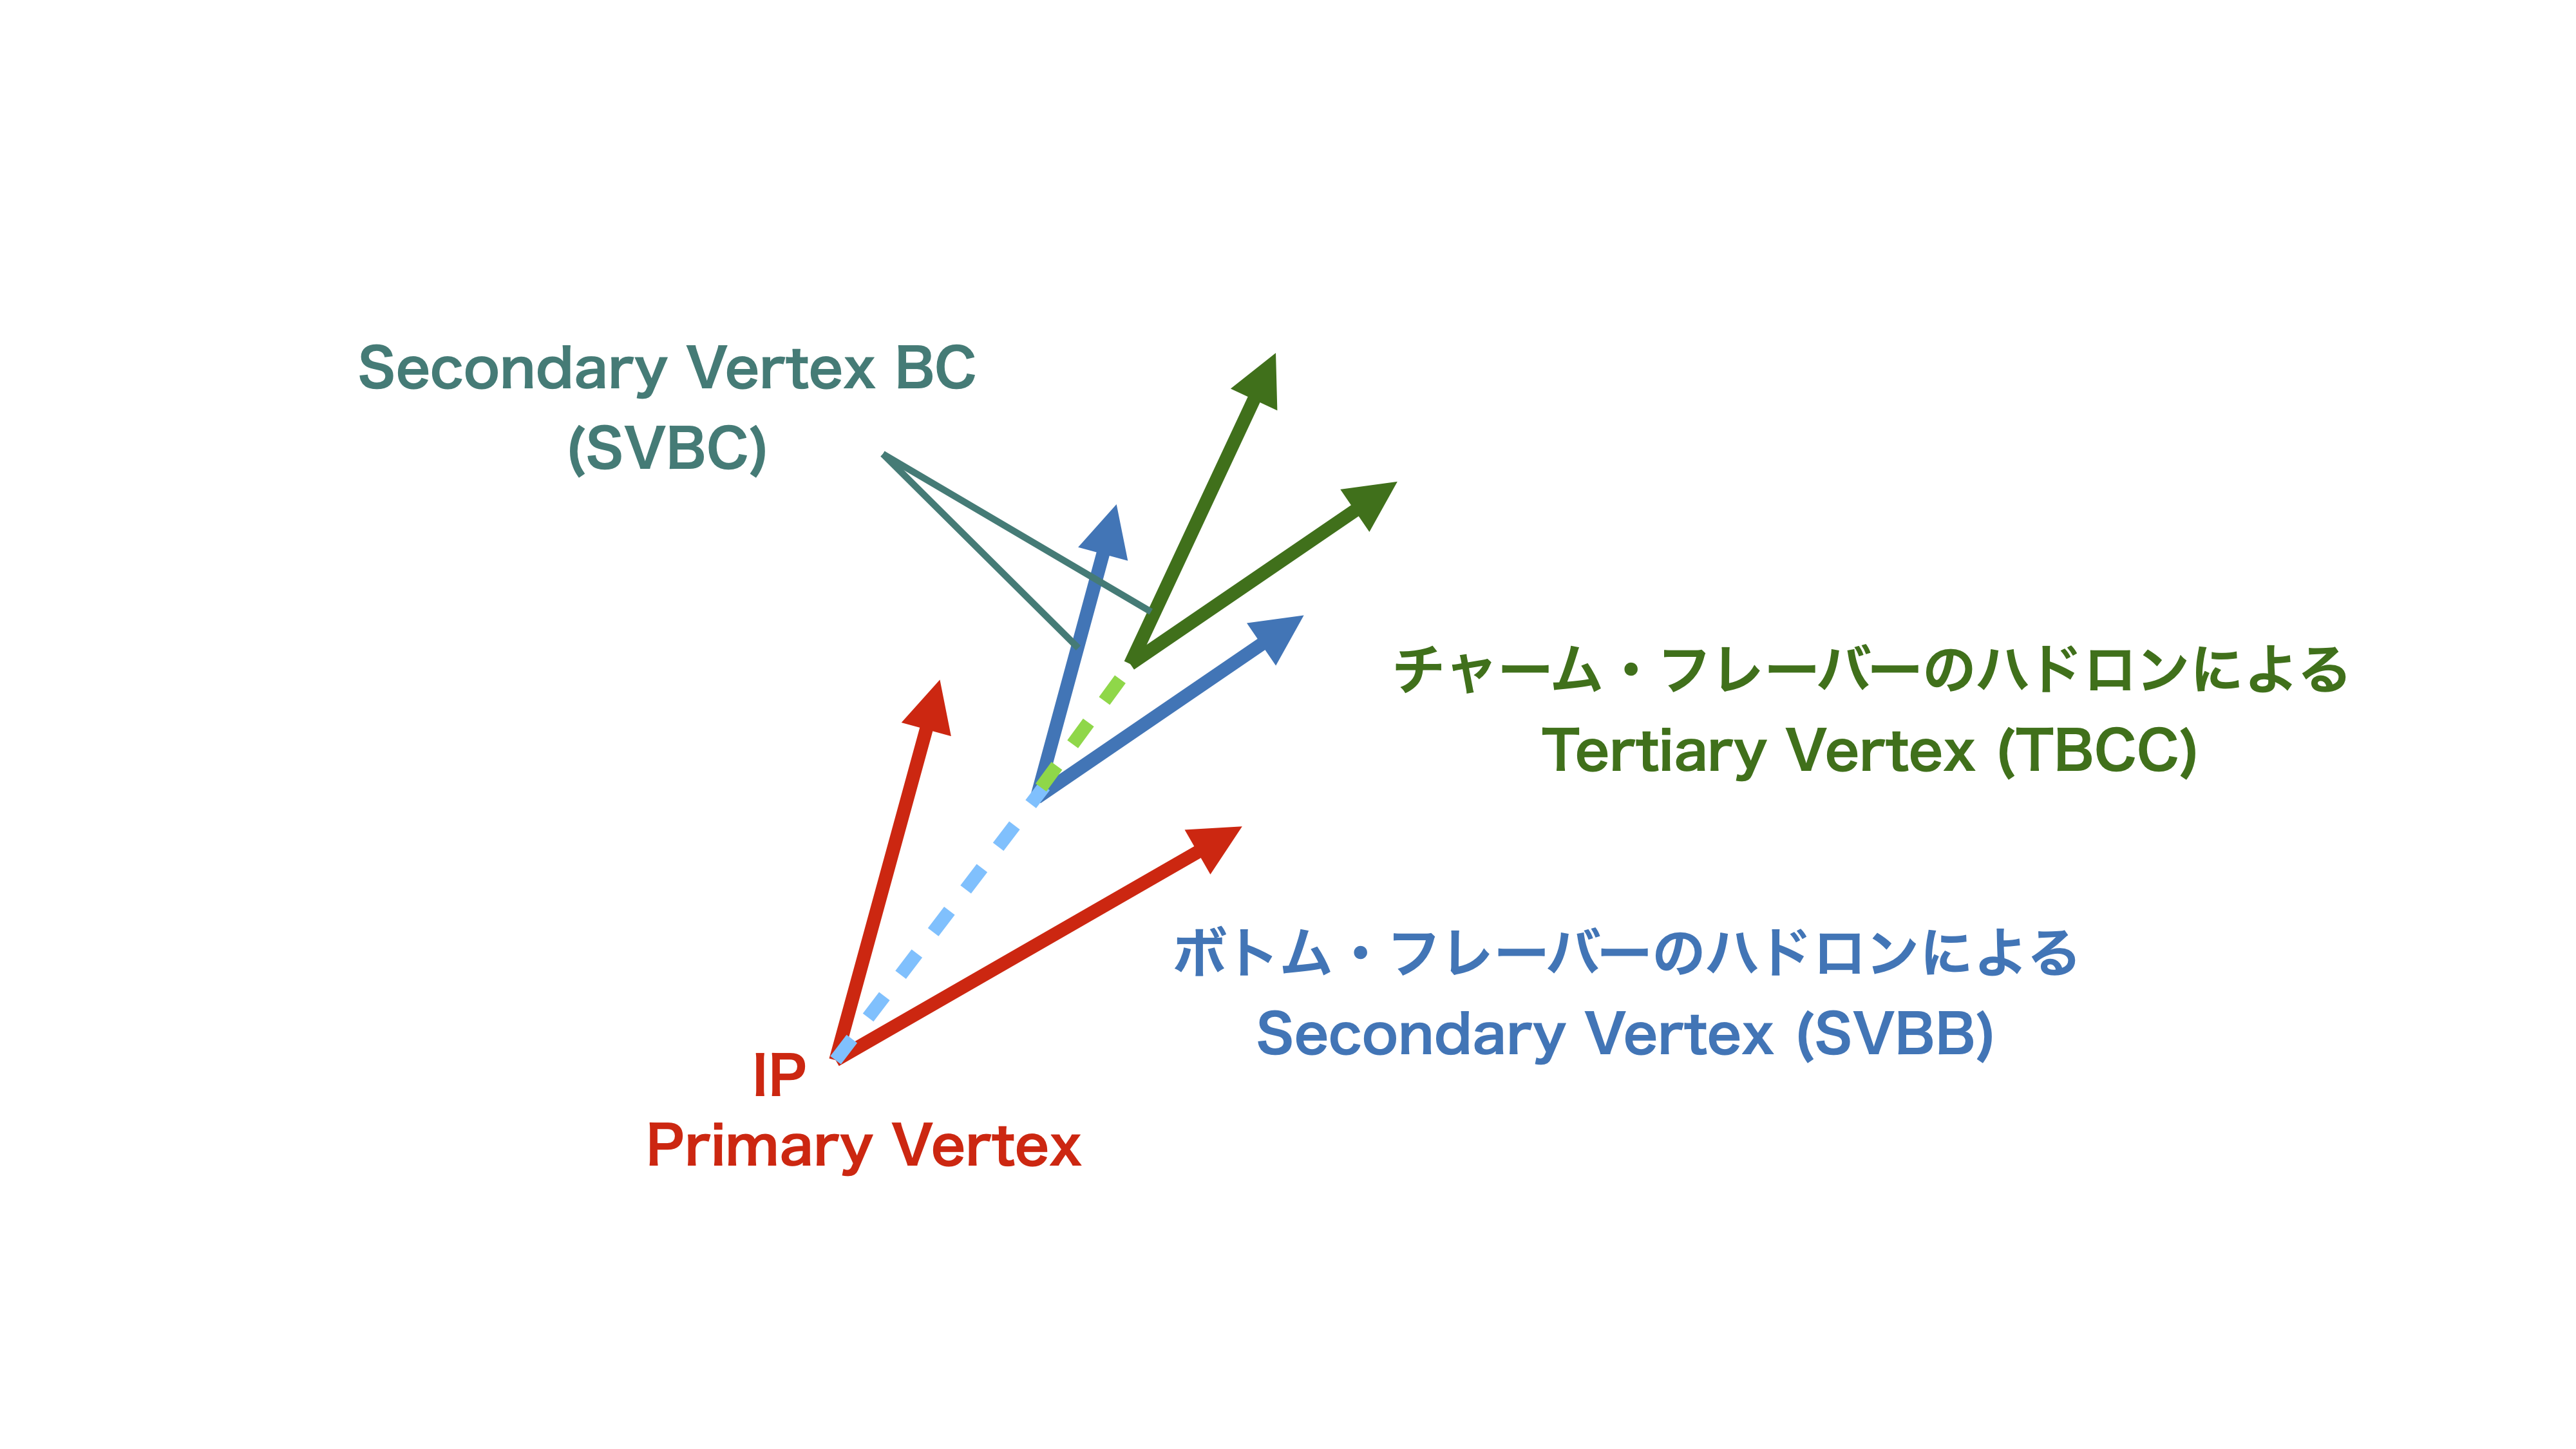
\includegraphics[trim = 0 100 0 50, width=0.9\textwidth]{Figure/3Networks/3-3-0-1SecondaryVertexBC.png}
 \caption{終状態$\rm b\bar{b}$での崩壊点}
 \label{3-3-0-1SecondaryVertexBC}
\end{figure}

崩壊点の位置についての訓練データを作成するに当たって、正解ラベルとしてLCFIPlusのフィッティングで得られる計算値を用いた。
こちらは回帰によって値を再現し、崩壊点の種類の補助として活用する。
ここでは崩壊点の位置としてImpact Parameter (IP) からの距離を使用した。

%%%%%%%%%%%%%%%%%%%%%%%%%%%%%%%%%%%%%%%%%%%%%%%%%%%%%%%%%%%%%%%%%%%%%%%%
\subsection{ネットワークの構造} \label{Net:PM:StructureofPM}

飛跡対についてのネットワークは非常にシンプルなフィードフォーワードニューラルネットワーク構造のものを使用した。
ネットワークの概略図を図\ref{3-3-1-1PairModel}に示す。

\begin{figure}[htbp]
 \centering
 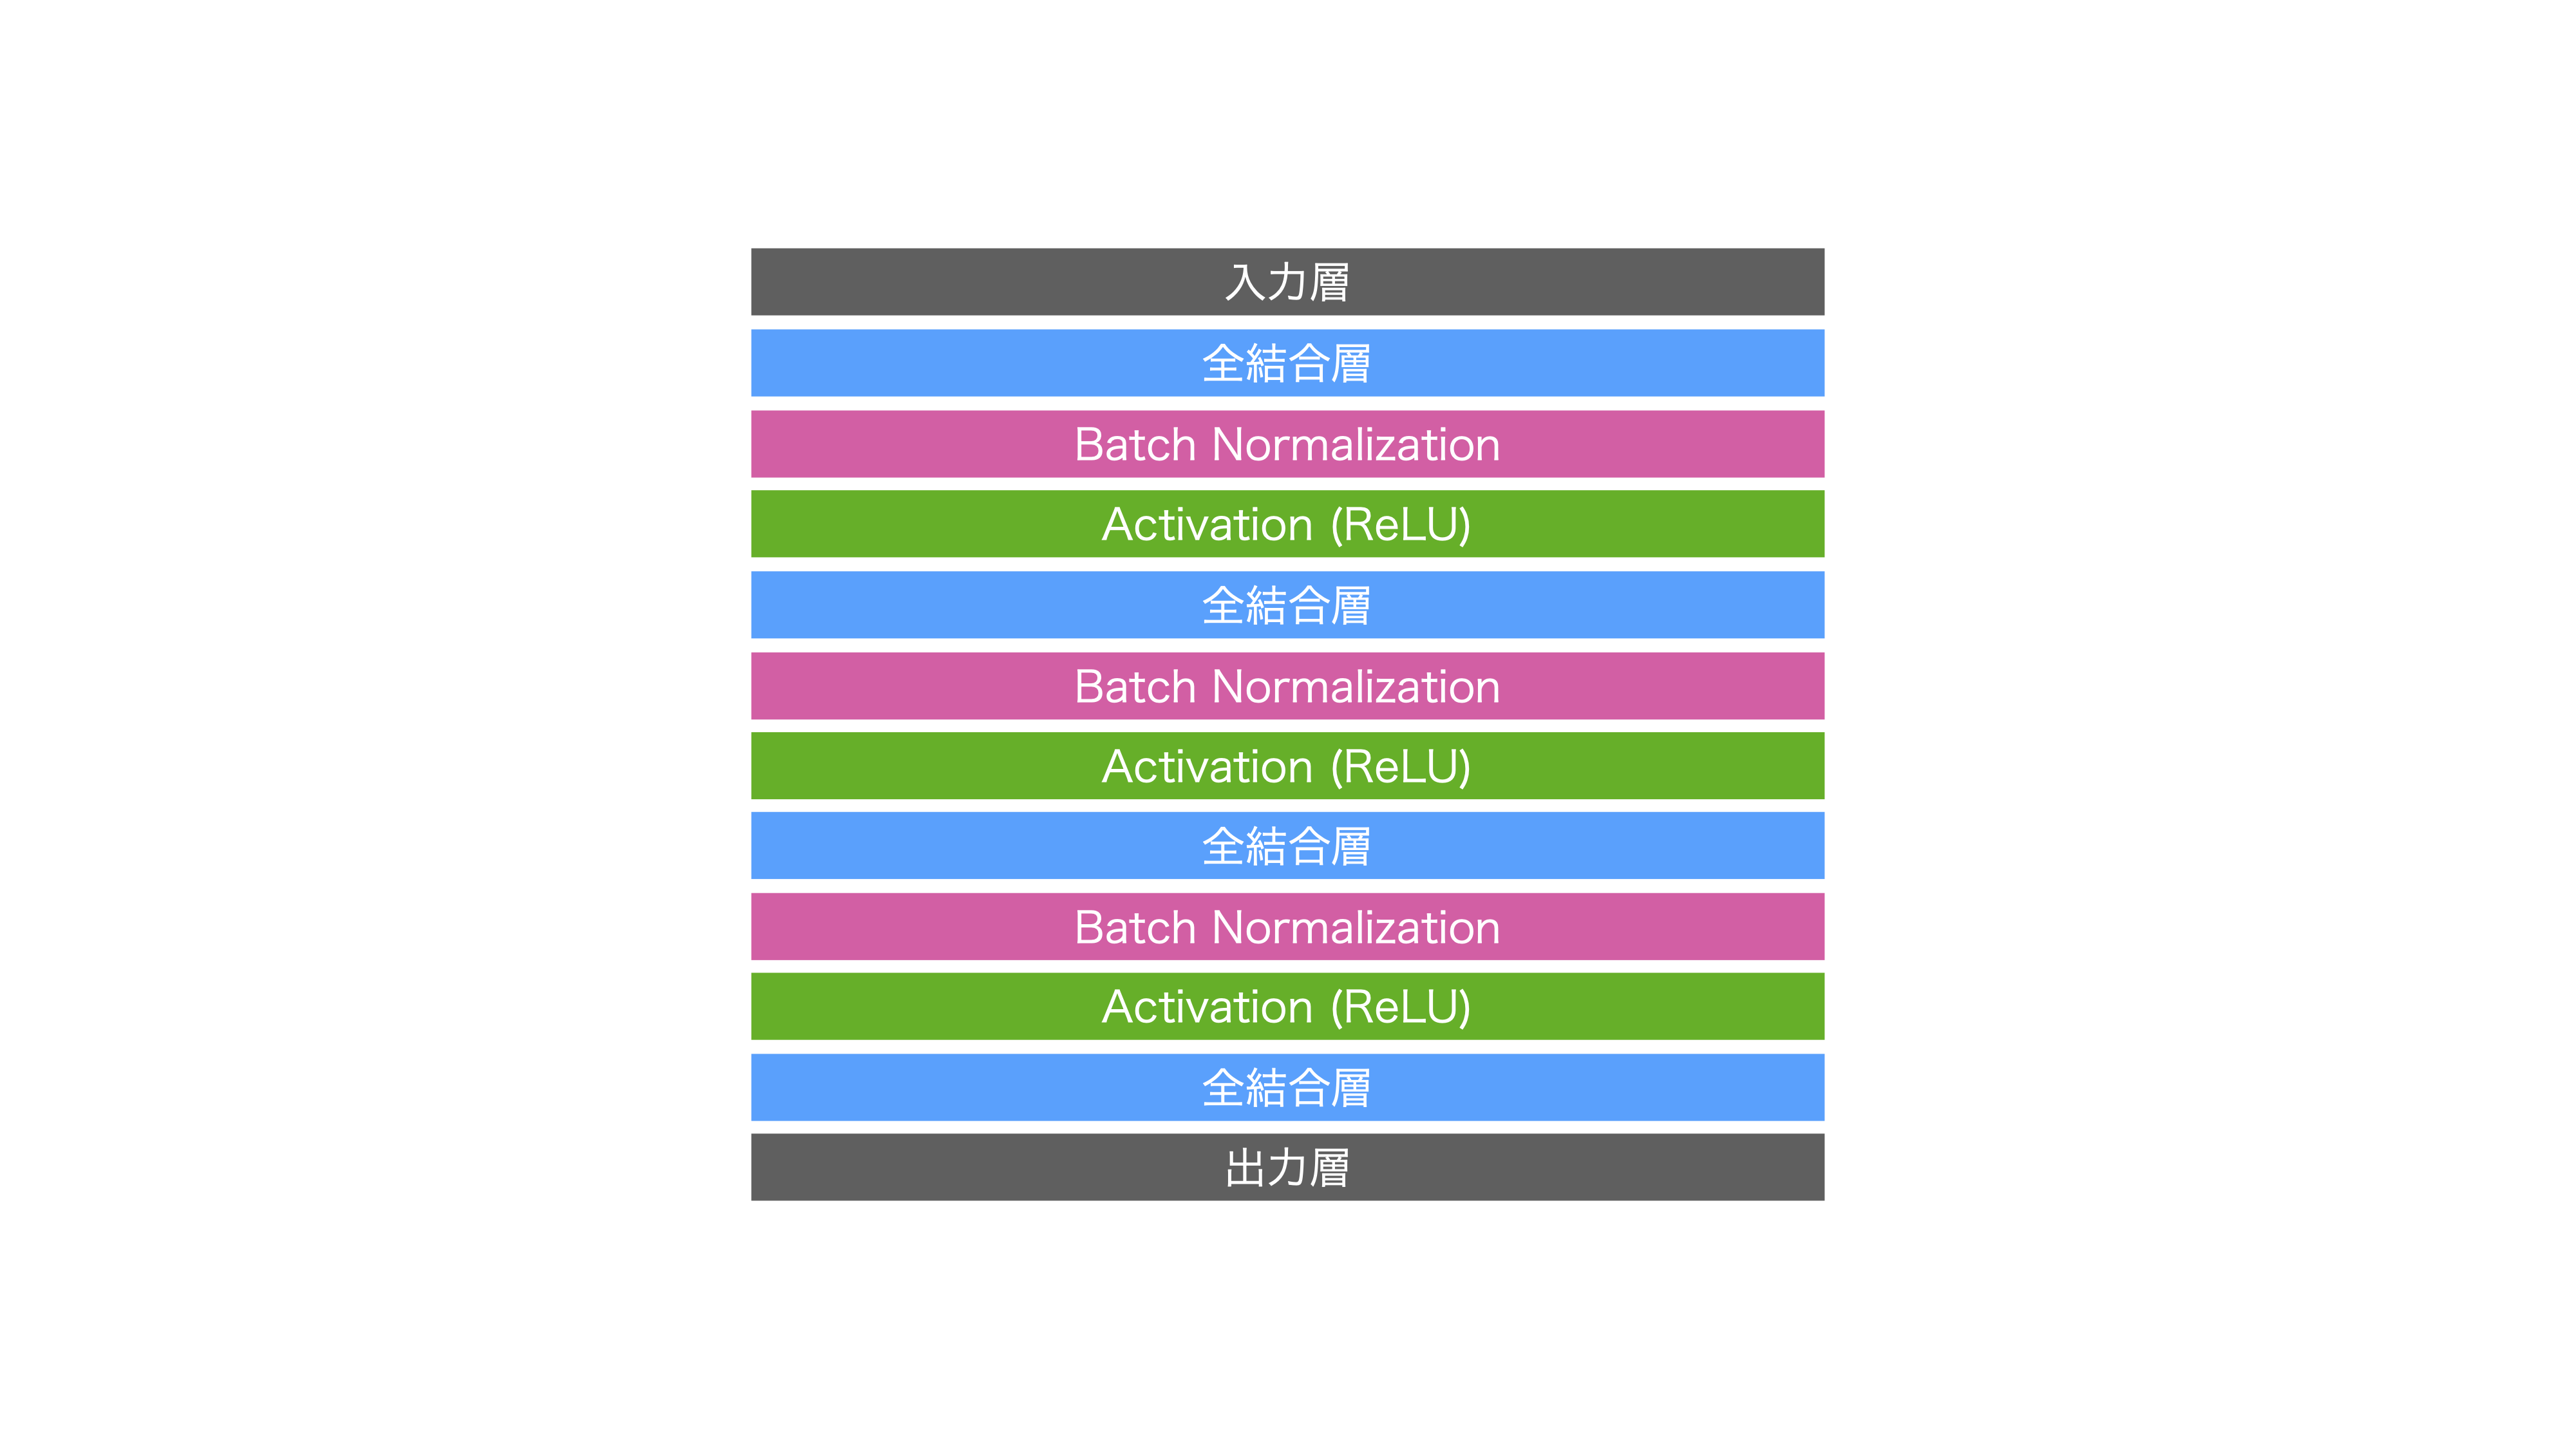
\includegraphics[trim = 100 100 100 50, width=0.9\textwidth]{Figure/3Networks/3-3-1-1PairModel.png}
 \caption{飛跡対についてのネットワークの概略図}
 \label{3-3-1-1PairModel}
\end{figure}

前述したように出力は、7クラス分類と回帰1つである。
7クラスの内訳はNC・PV・SVCC・SVBB・TVCC・SVBC・Othersである。
回帰では崩壊点の位置を予想している。
また、過学習 (Over fitting) を避ける為、Batch Normalization\cite{BatchNormalizationpaper}を全結合層の後ろに配置している。
過学習とは、ネットワークが過度に訓練データに適合してしまい、検証データやテストデータへの汎化性能が悪化してしまう教師あり学習の問題の一つである。
また勾配消失への対策として、活性化関数は全てReLU関数を使用している。


%%%%%%%%%%%%%%%%%%%%%%%%%%%%%%%%%%%%%%%%%%%%%%%%%%%%%%%%%%%%%%%%%%%%%%%%
\subsection{ネットワークの学習と戦略} \label{Net:PM:TrainingandStrategyofPM}

訓練データは事象中の全ての飛跡対の組み合わせを考える。

ここで二つの事柄に注意せねばならない。
一つは、この出力は二つの終状態$\rm b\bar{b}$と$\rm c\bar{c}$を合わせたものという点である。
もう一つは、分類クラスの数の比が"Not Connected (NC)"や"Primary Vertex (PV)"が支配的な不均衡データ (Imbalanced Data) となるという点である。
各終状態での分類クラスの数の比を図\ref{3-3-2-1ImbalancedData}に示す。

\begin{figure}[htbp]
 \centering
 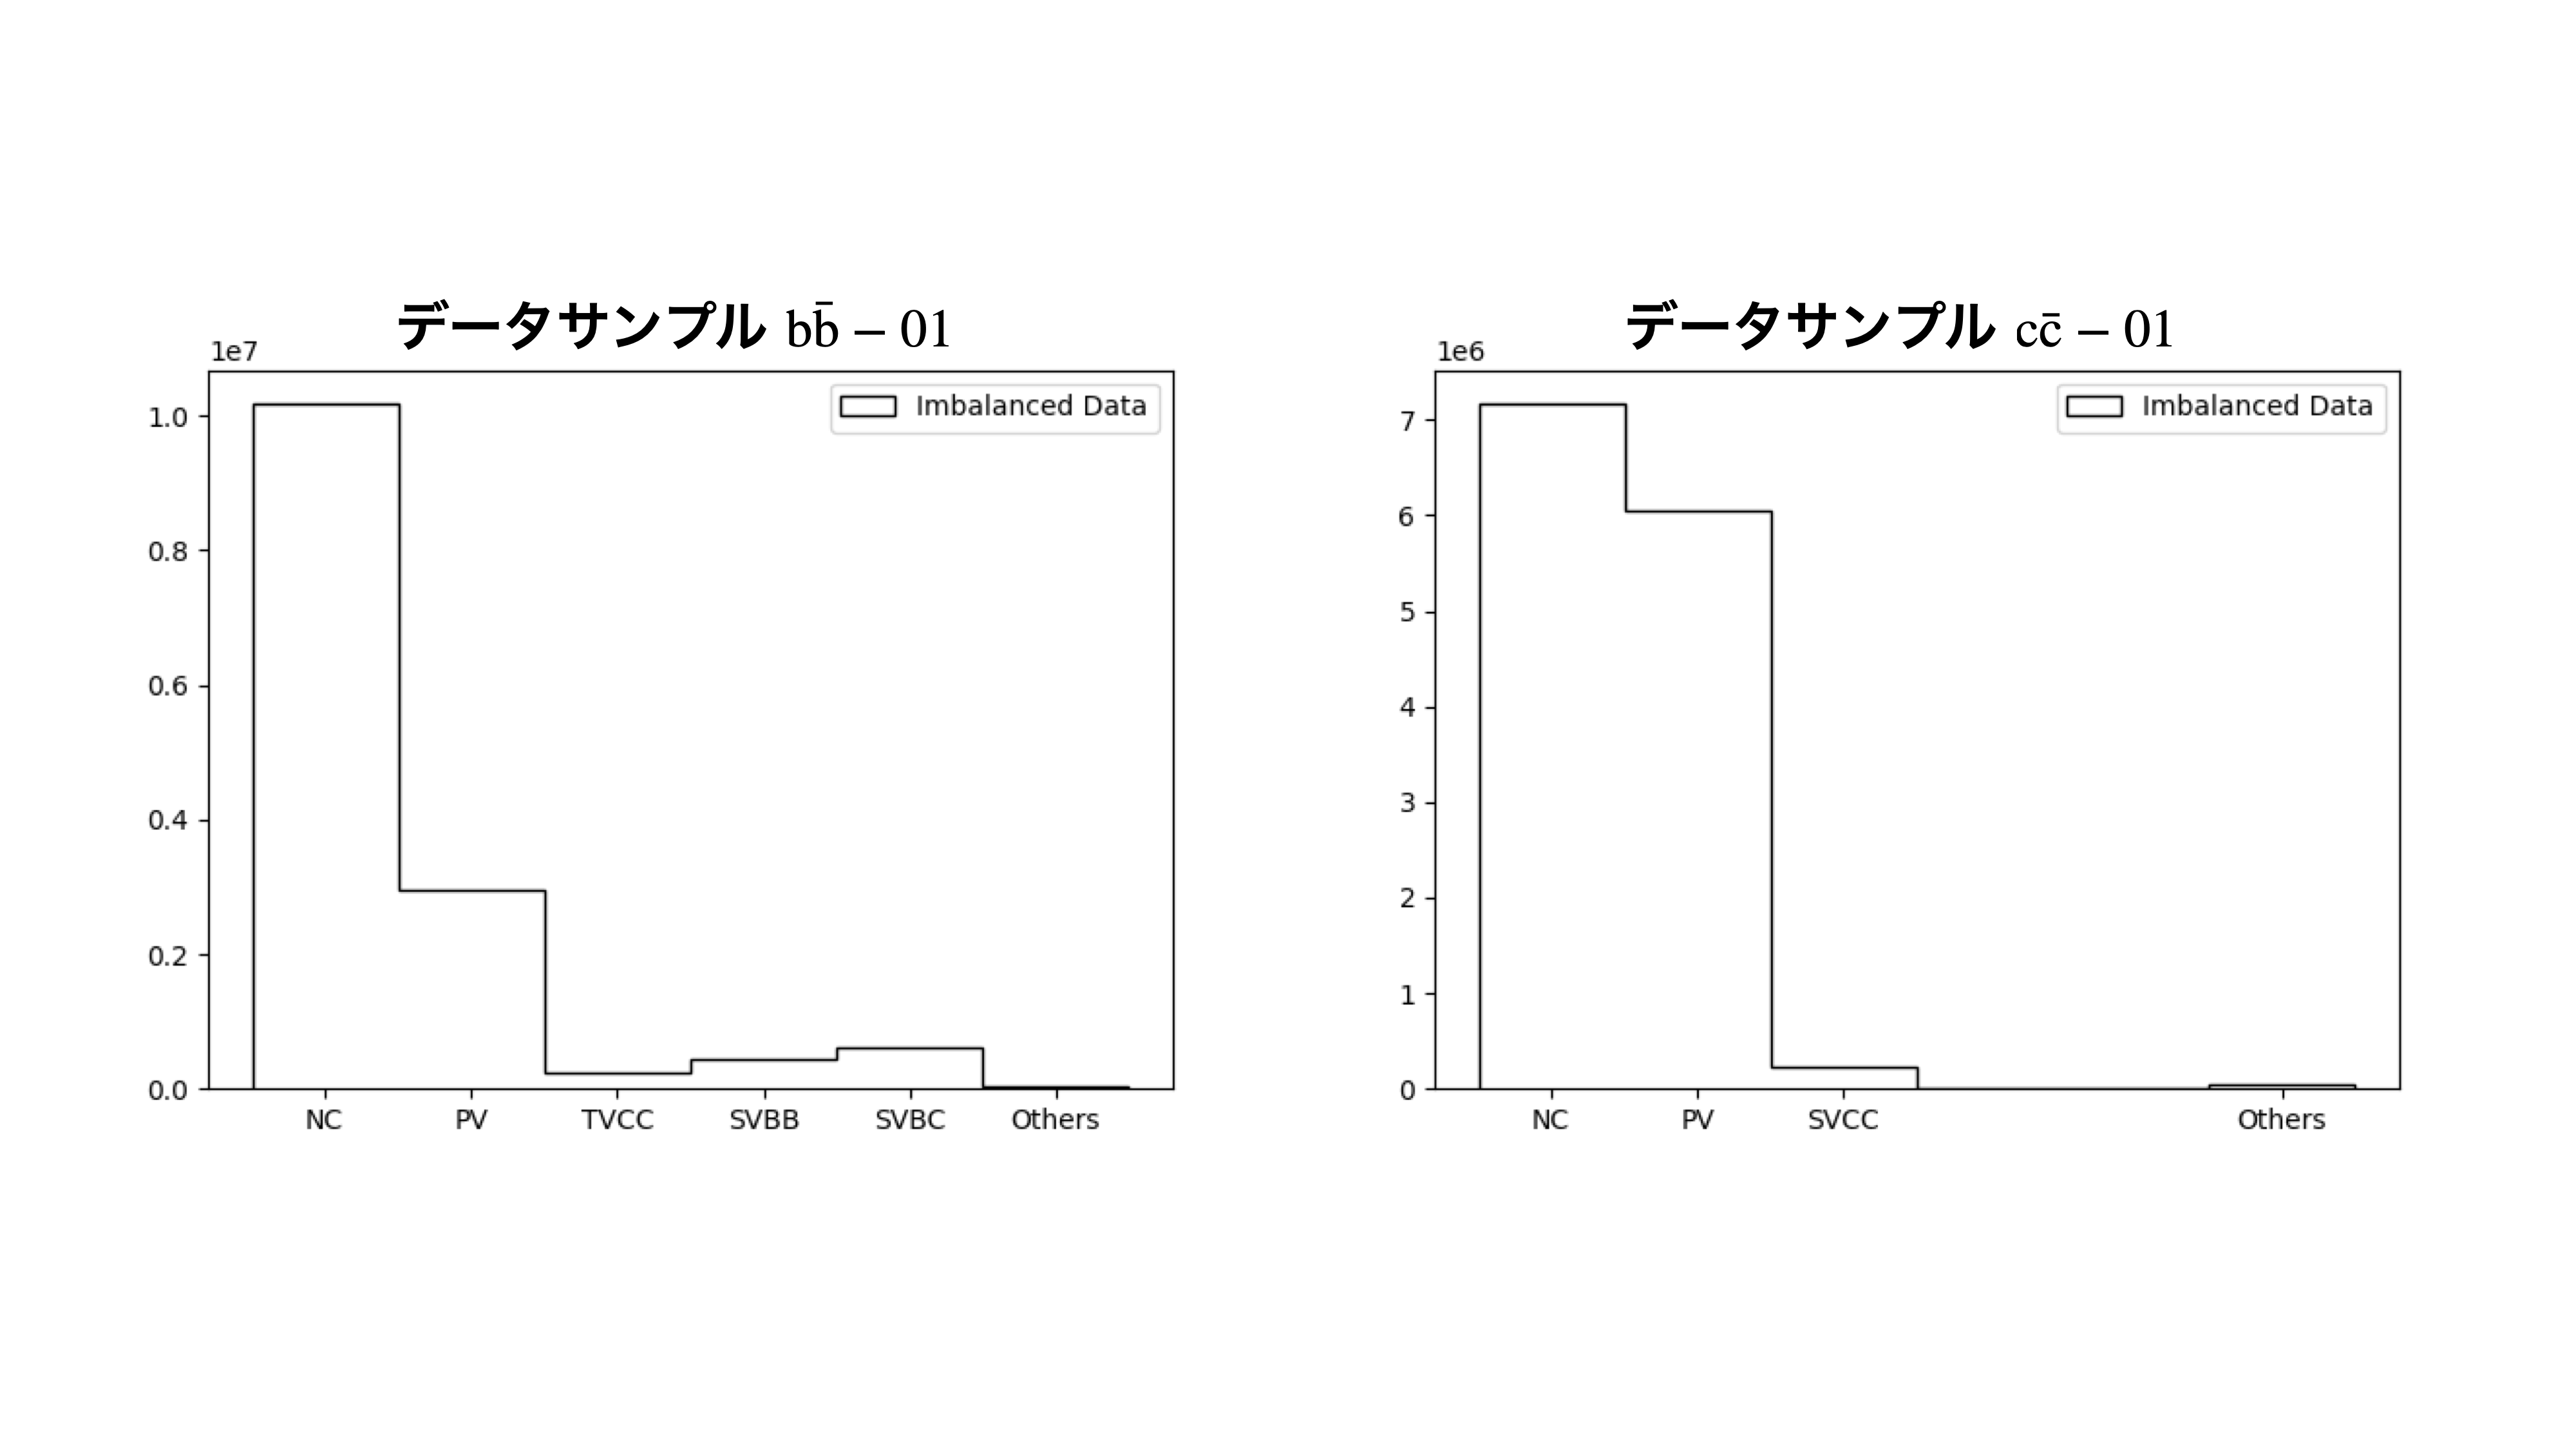
\includegraphics[width=1.0\textwidth]{Figure/3Networks/3-3-2-1ImbalancedData.png}
 \caption{各終状態での分類クラスの数の比}
 \label{3-3-2-1ImbalancedData}
\end{figure}

このような不均衡データについては、少数クラスのデータをかさ増しするOversampling、多数クラスのデータを間引くUndersampling、損失関数のコストに重みをつけるコスト考慮型学習の主に三つの対応策が存在する。
OversamplingやUndersamplingは過学習や情報の欠損などの問題を抱えているため、基本的に本研究ではコスト考慮型学習を用いた。
ただし、二つの終状態のデータを単純に足し合わせた場合、共通する"NC"や"PV"がより顕著になり、"SV"などの分類が不十分になると考えられる。
このため"NC"や"PV"に関しては二つの終状態を足し合わせた後、二つの値の平均値となるようにランダムサンプリングを行った。

\begin{figure}[htbp]
 \centering
 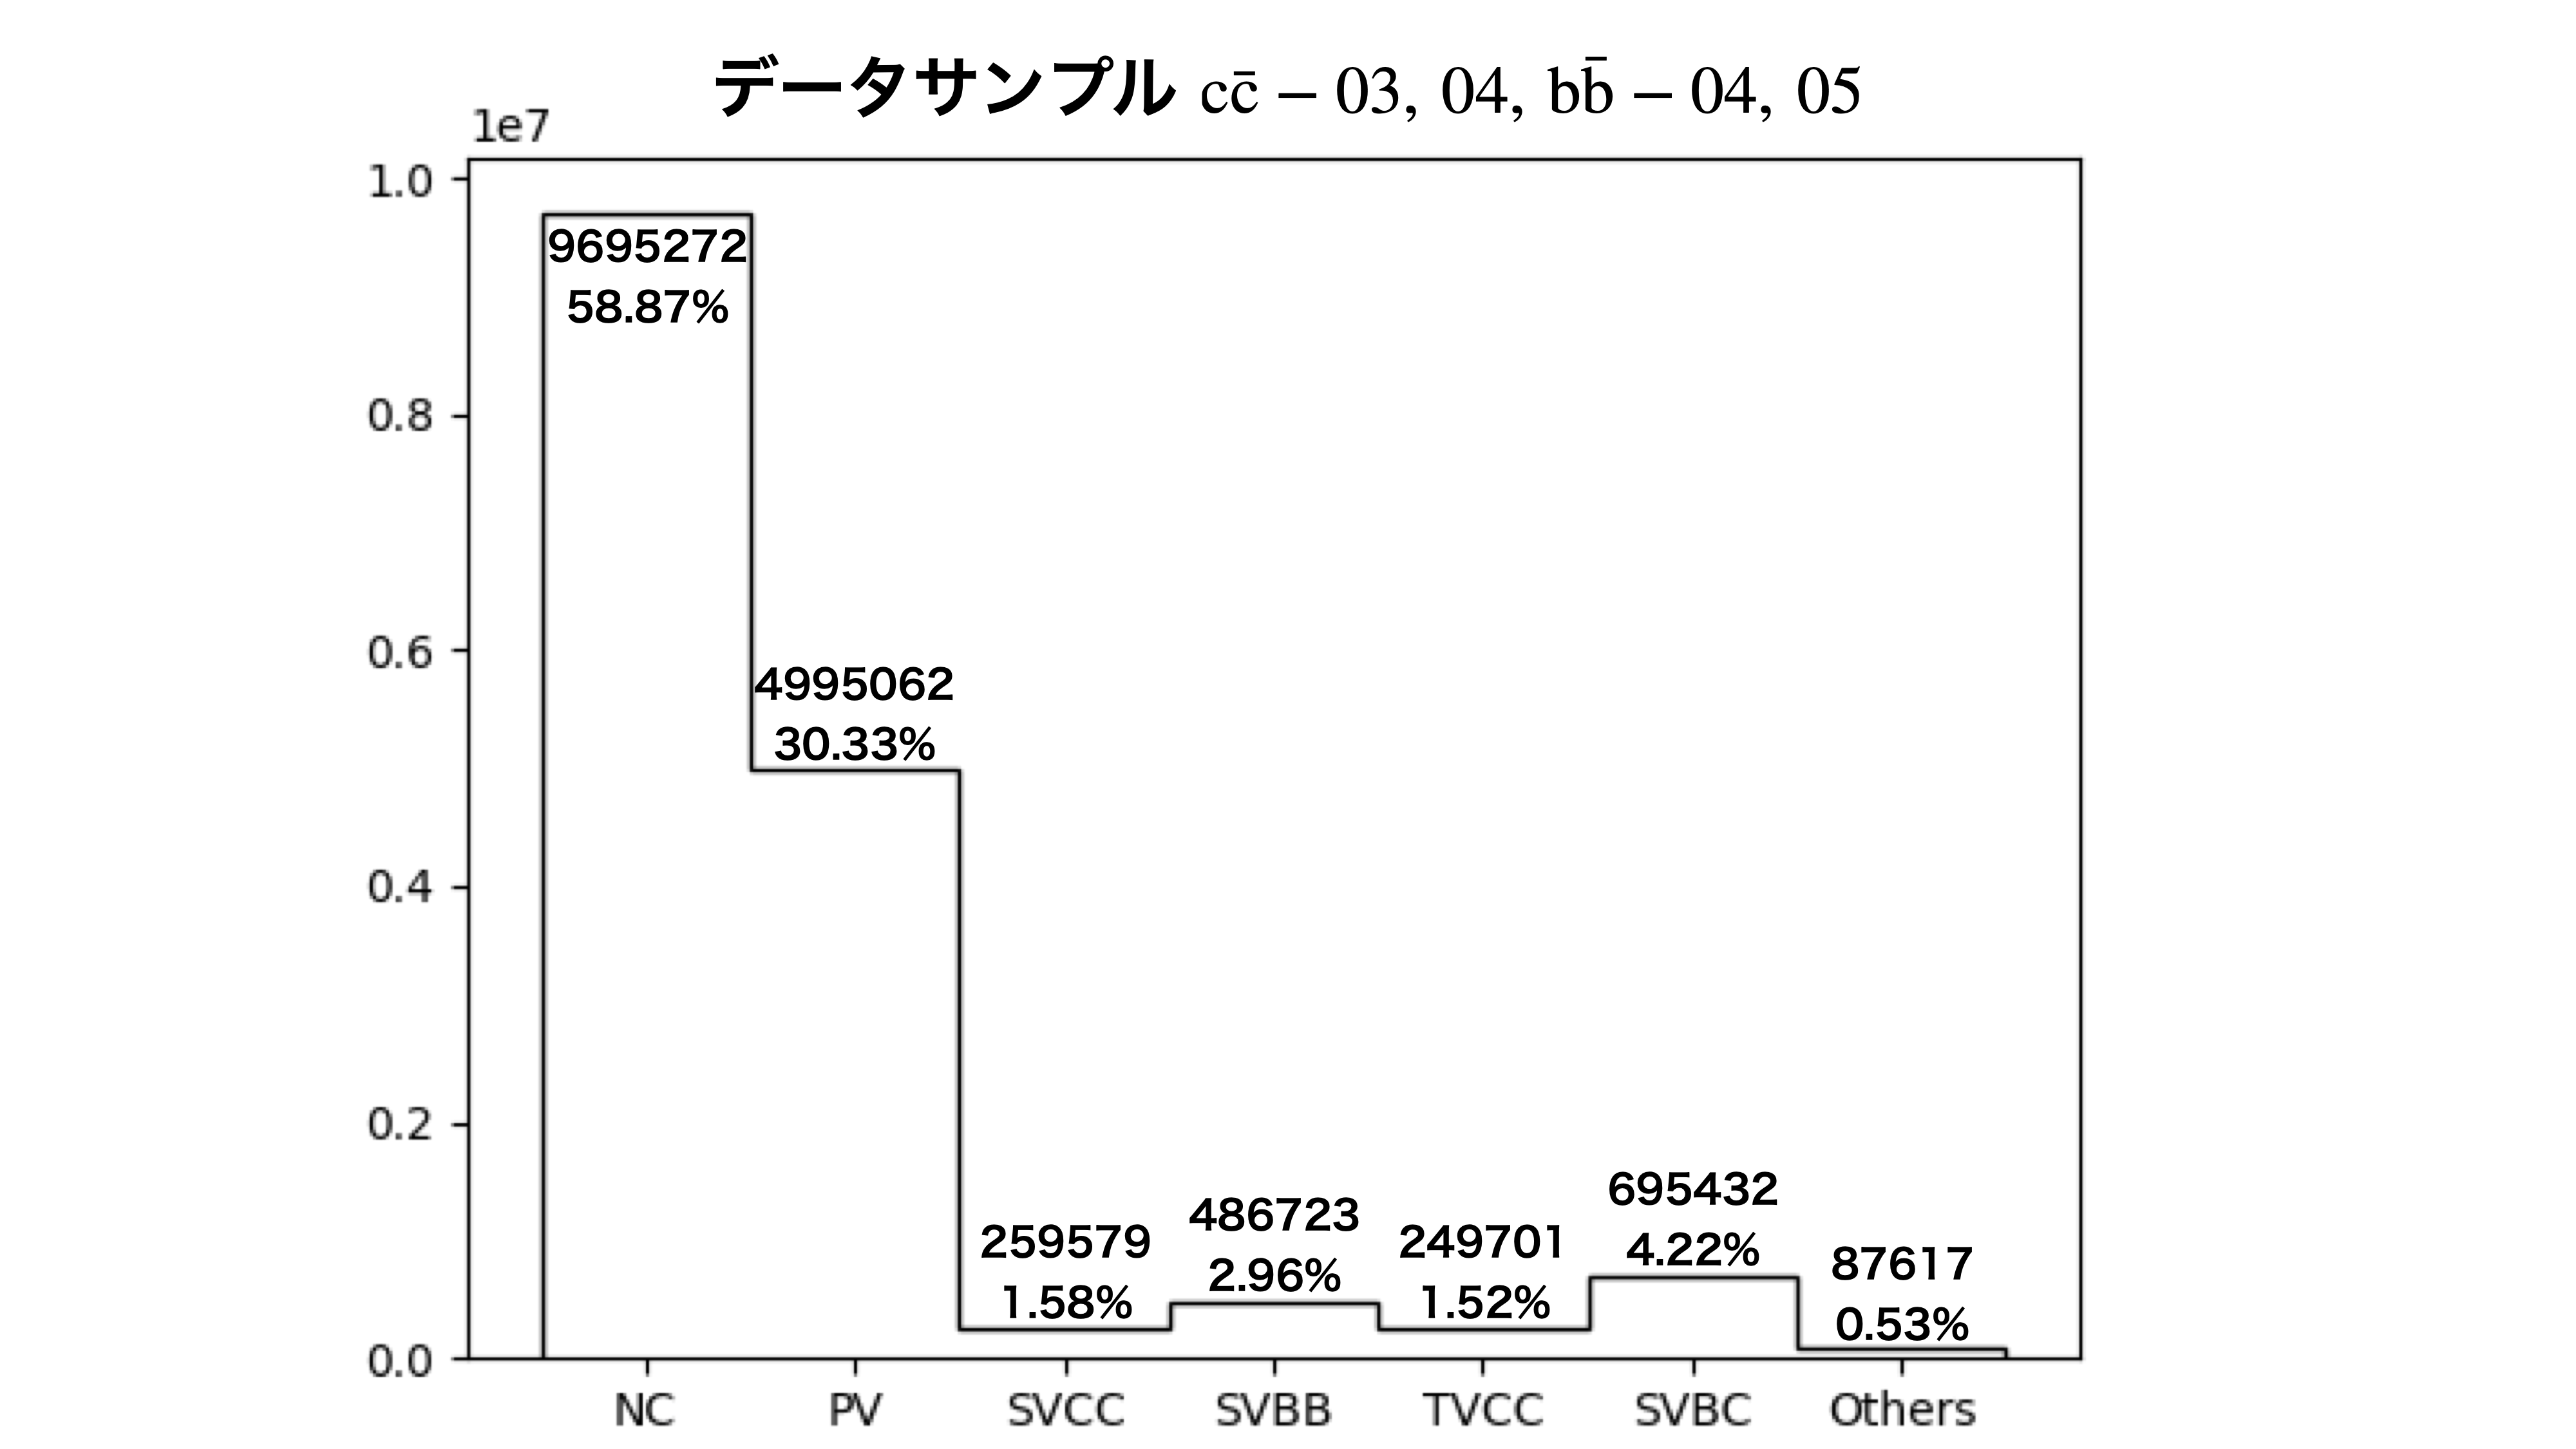
\includegraphics[width=1.0\textwidth]{Figure/3Networks/3-3-2-2ImbalancedData.png}
 \caption{訓練データでの分類クラスの数の比}
 \label{3-3-2-2ImbalancedData}
\end{figure}

損失関数の各クラスへの重みは分類クラスの数の比の逆数を使用した。
\begin{equation}
 \begin{split}
 L = & - 0.0090\  t_{\rm NC} \log{(y_{\rm NC})} - 0.0175\  t_{\rm PV} \log{(y_{\rm PV})} \\
       & - 0.3375\  t_{\rm SVCC} \log{(y_{\rm SVCC})} - 0.1800\  t_{\rm SVBB} \log{(y_{\rm SVBB})}\\
       & - 0.3509\  t_{\rm TVCC} \log{(y_{\rm TVCC})} - 0.1260\  t_{\rm SVBC} \log{(y_{\rm SVBC})}\\
       & - 1.0\  t_{\rm Others} \log{(y_{\rm Others})}\\
 \end{split}
\end{equation}

飛跡対についてのネットワークで使用したハイパーパラメータを表\ref{HyperparametersforPairModel}に示す。

\begin{table}[htb]
 \centering
 \small
  \begin{tabular}{c c}\hline
    最適化手法 & SGD\\
    学習率 & 0.001\\
    エポック数 & 2500\\
    バッチサイズ & 1024\\
    ノード数 & 256\\ \hline
  \end{tabular}
  \caption{飛跡対についてのネットワークで使用したハイパーパラメータ}
  \label{HyperparametersforPairModel}
\end{table}

重み更新の最適化手法として、SGDを用いた。
これは、Adamなどでは収束が早すぎ、過学習になる恐れがあったためである。
エポック数は過学習にならない程度の値を選択した。
エポック数を横軸に、正答率と損失を縦軸にプロットした学習曲線を図\ref{3-3-2-2TrainingCurve}に示す。

%\begin{figure}[htbp]
 %\centering
 %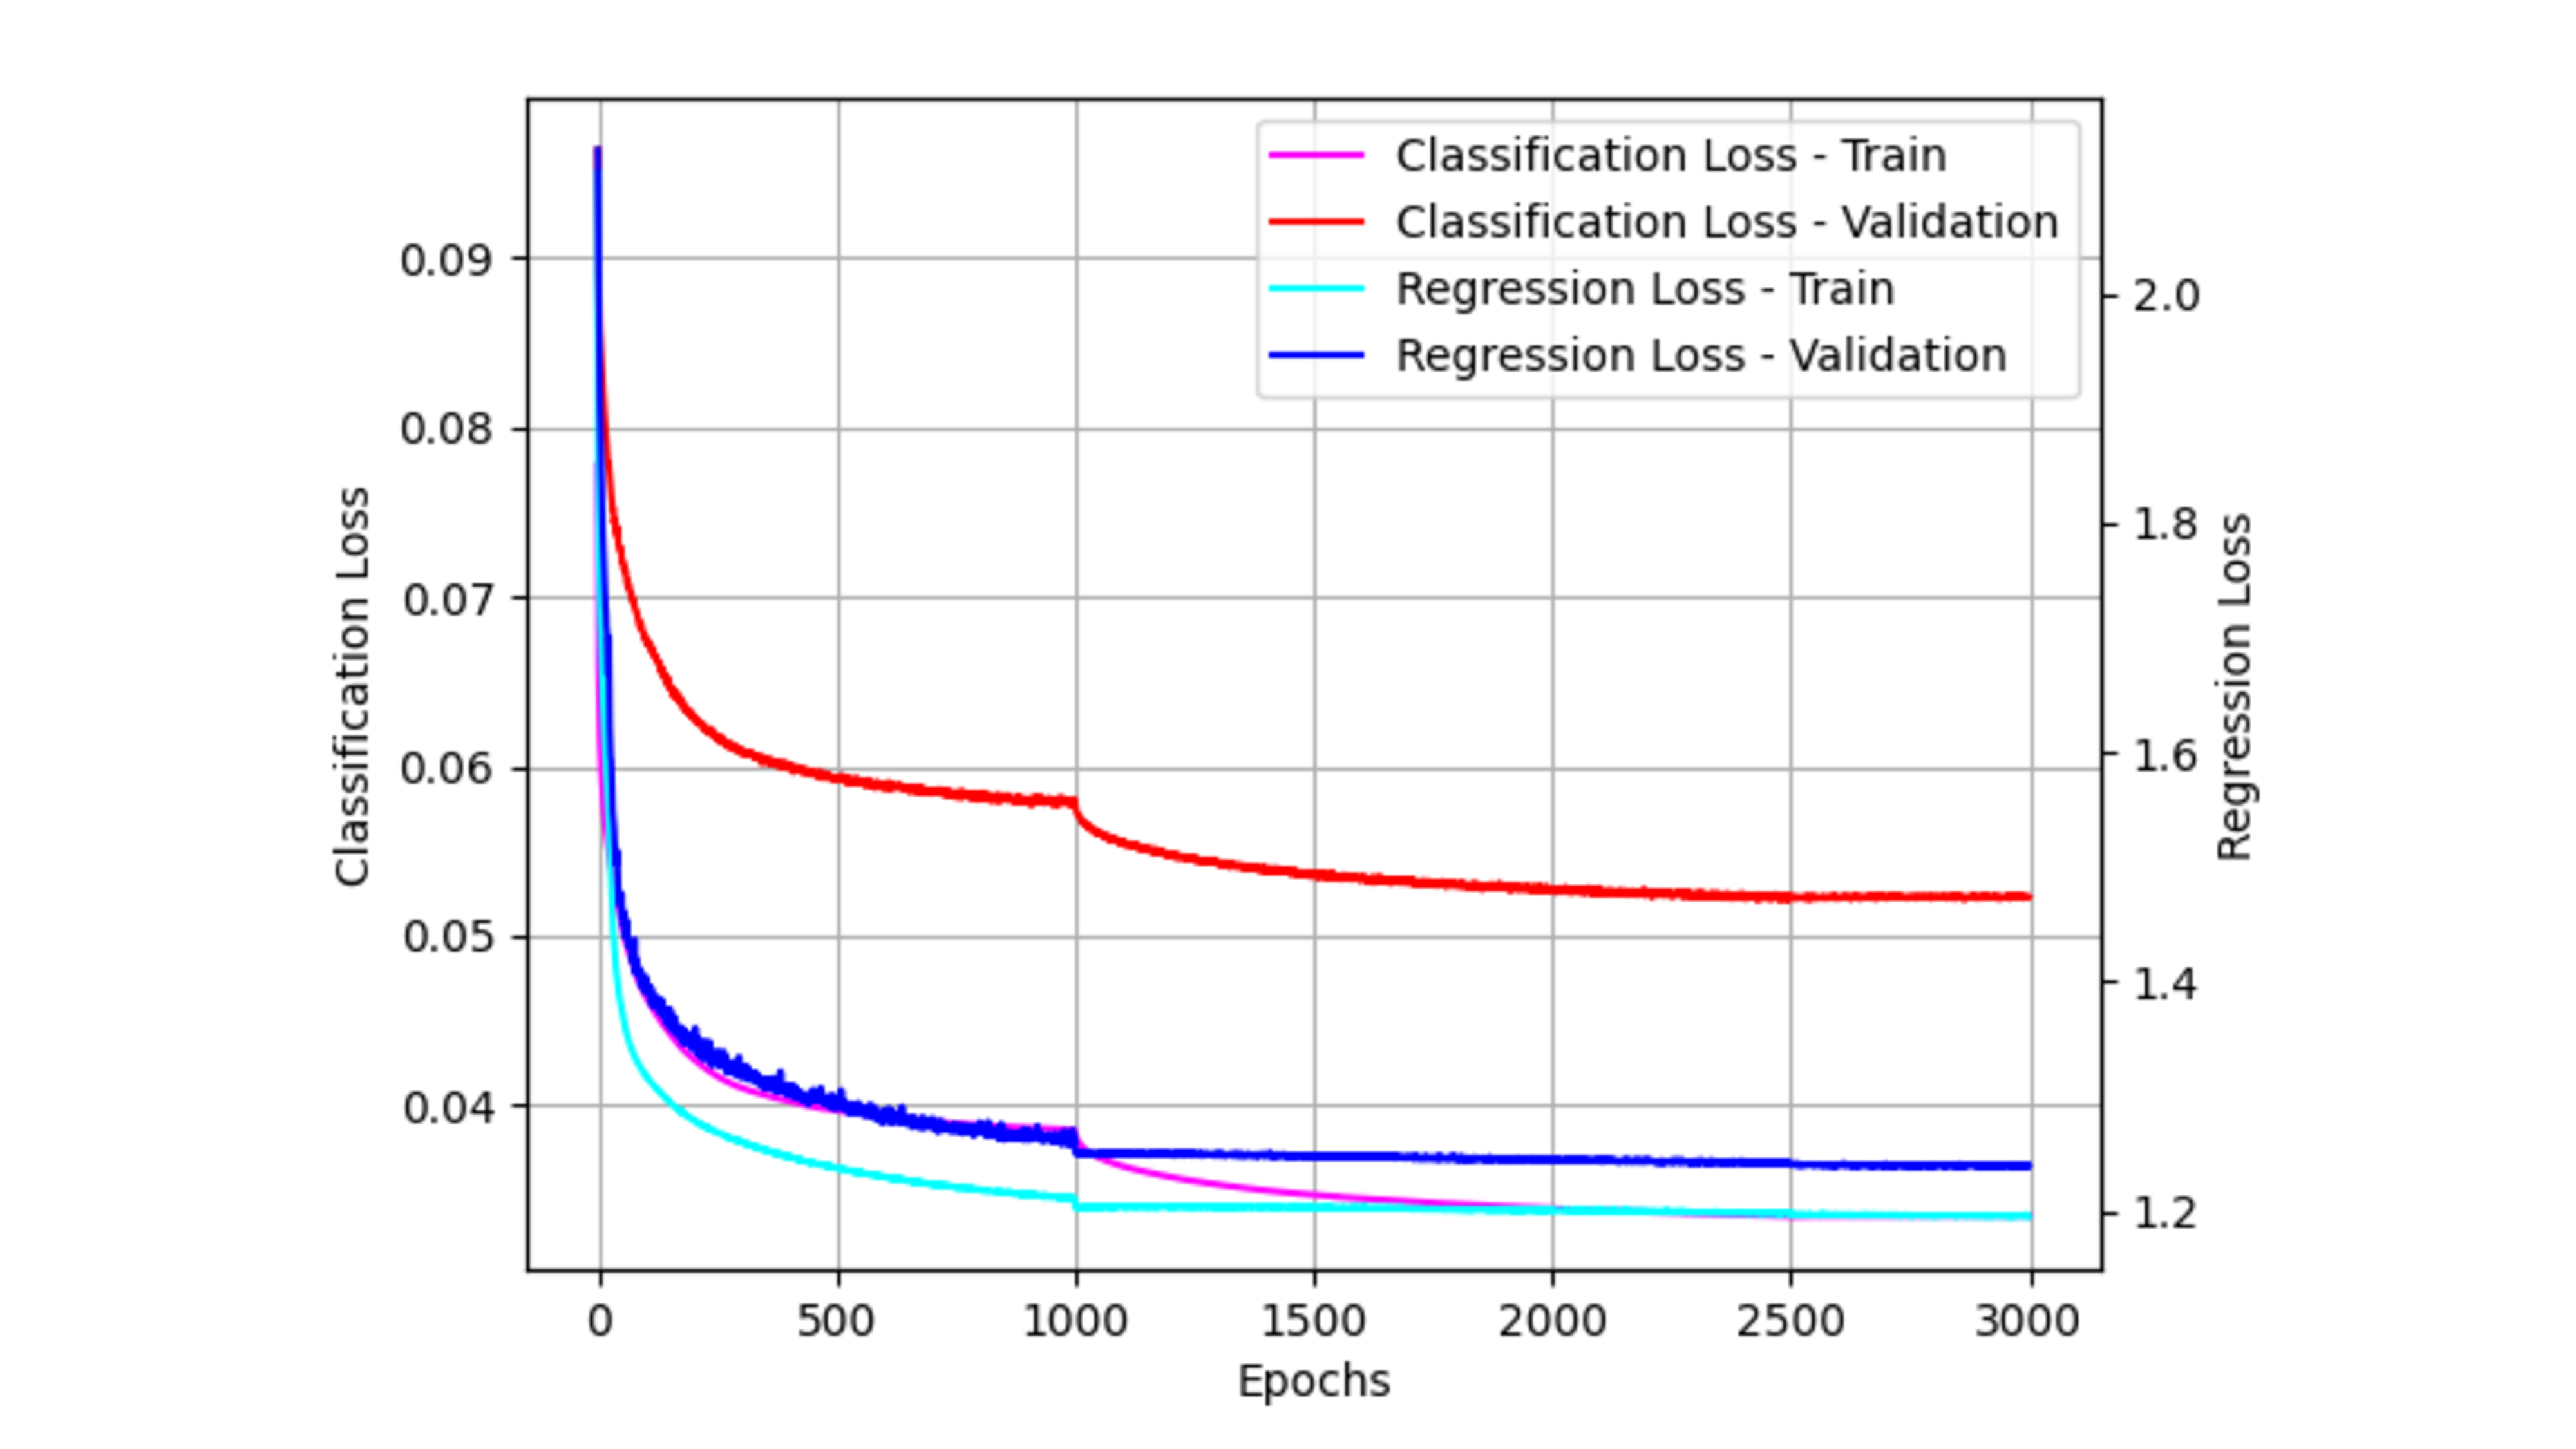
\includegraphics[width=1.0\textwidth]{Figure/3Networks/3-3-2-2TrainingCurve.png}
 %\caption{飛跡対についてのネットワークの学習曲線}
 %\label{3-3-2-2TrainingCurve}
%\end{figure}


%%%%%%%%%%%%%%%%%%%%%%%%%%%%%%%%%%%%%%%%%%%%%%%%%%%%%%%%%%%%%%%%%%%%%%%%
\subsection{ネットワークの性能} \label{Net:PM:PerformanceofPM}

ここではネットワークの性能を評価する。

まず、ネットワークがどの変数を見ているかについて評価する。
ここでは、崩壊点の位置とトラック・パラメータの共分散行列について調査を行う。
崩壊点を分類する上で崩壊点の位置についての情報は非常に重要である。
特に各Secondary Vertexを識別するためにネットワークは、トラック・パラメータから粒子の飛跡を再構成し、それらが交点を持つかを評価する必要がある。
また、ネットワークに誤差などの情報を取り入れることは困難であると言われており、本研究においても、ネットワークが共分散行列の情報を取り扱えているかを評価せねばならないと考える。

そのため、図\ref{3-3-3-1PairModels}のようなネットワーク、モデルA・モデルB・モデルC・モデルDを構築する。
モデルAとモデルDは図\ref{3-3-1-1PairModel}と同様の構造である。
モデルAでは飛跡についての全ての情報を使用し、モデルDでは共分散行列を取り除いた14個の変数を使用する。
モデルBはLCFIPlusで計算された崩壊点の位置を出力の直前の全結合層に使用している。
モデルBでは、訓練データの正解ラベルであるLCFIPlusで計算された崩壊点の位置を入力として使用しているため、出力は崩壊点の分類のみとしている。
モデルCはネットワークで予想された崩壊点の位置を出力の直前の全結合層に使用している。

\begin{figure}[htbp]
 \centering
  %\begin{tabular}{cccc}
  \begin{minipage}{1.0\textwidth}
  \centering
   \begin{minipage}{0.48\textwidth}
    \centering
    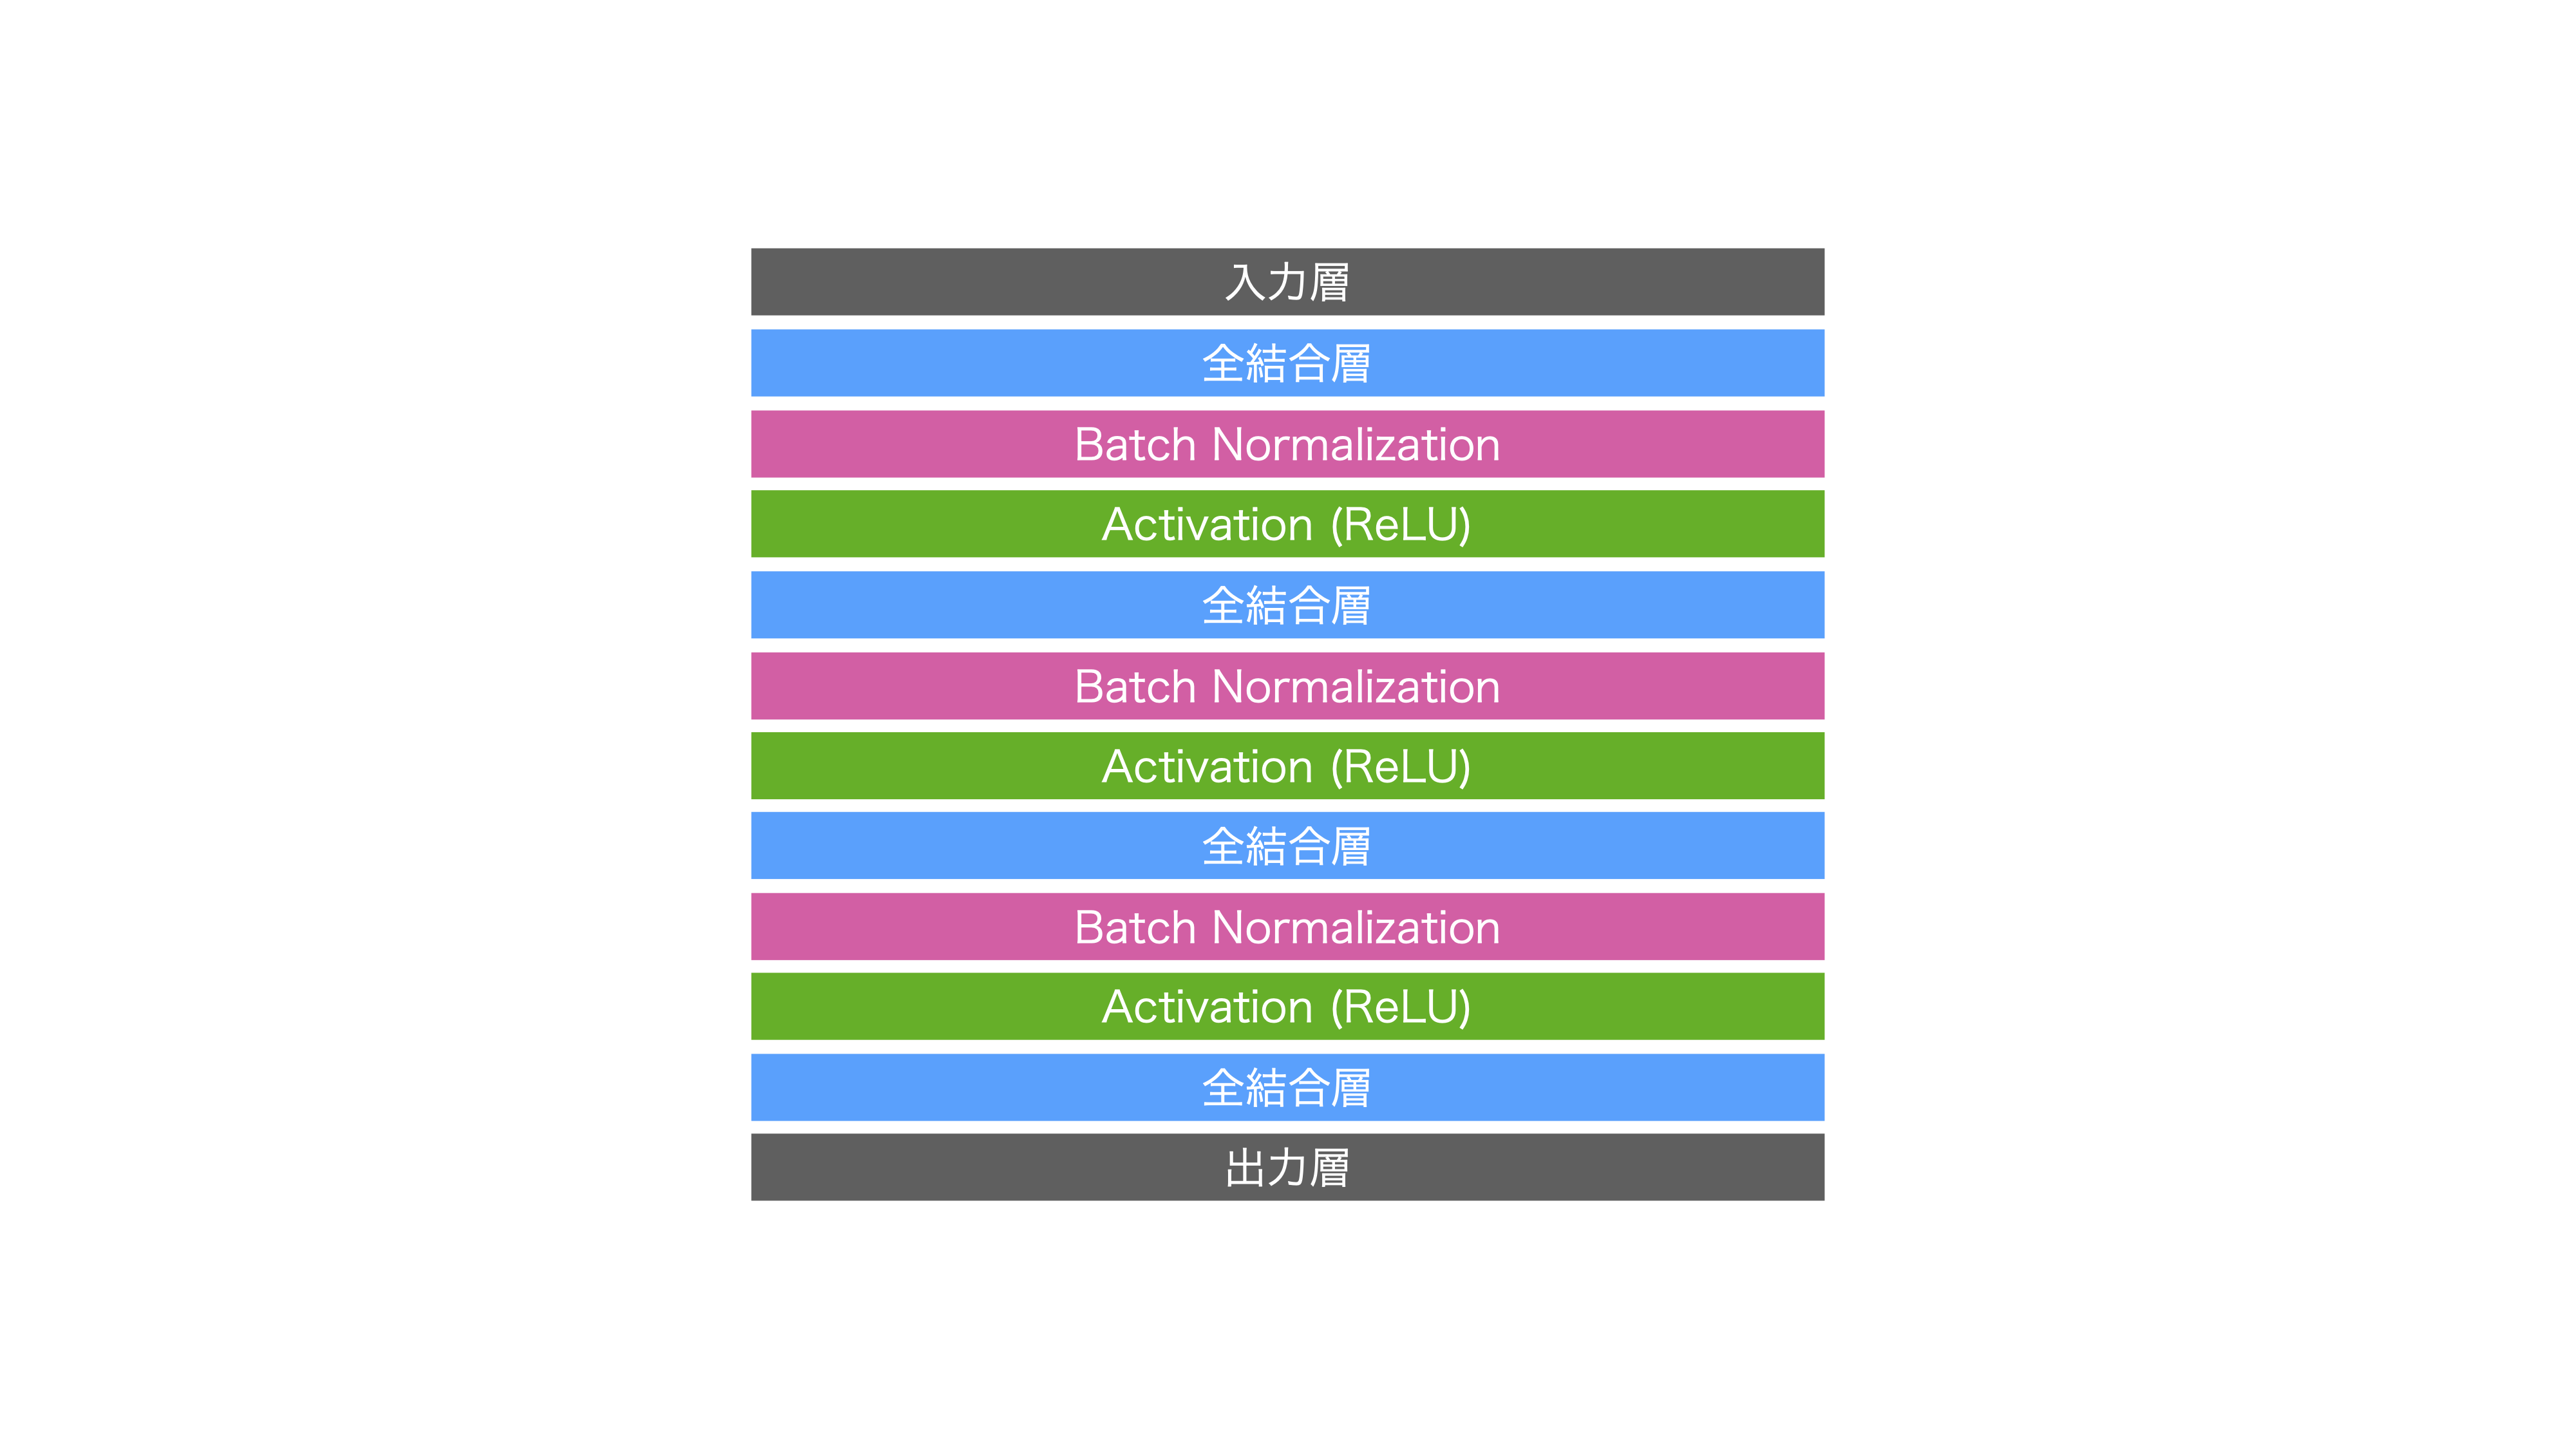
\includegraphics[width=1.0\textwidth, clip]{Figure/3Networks/3-3-1-1PairModel.png}
    \subcaption{モデルA}
   \end{minipage}
   \begin{minipage}{0.48\textwidth}
   \centering
    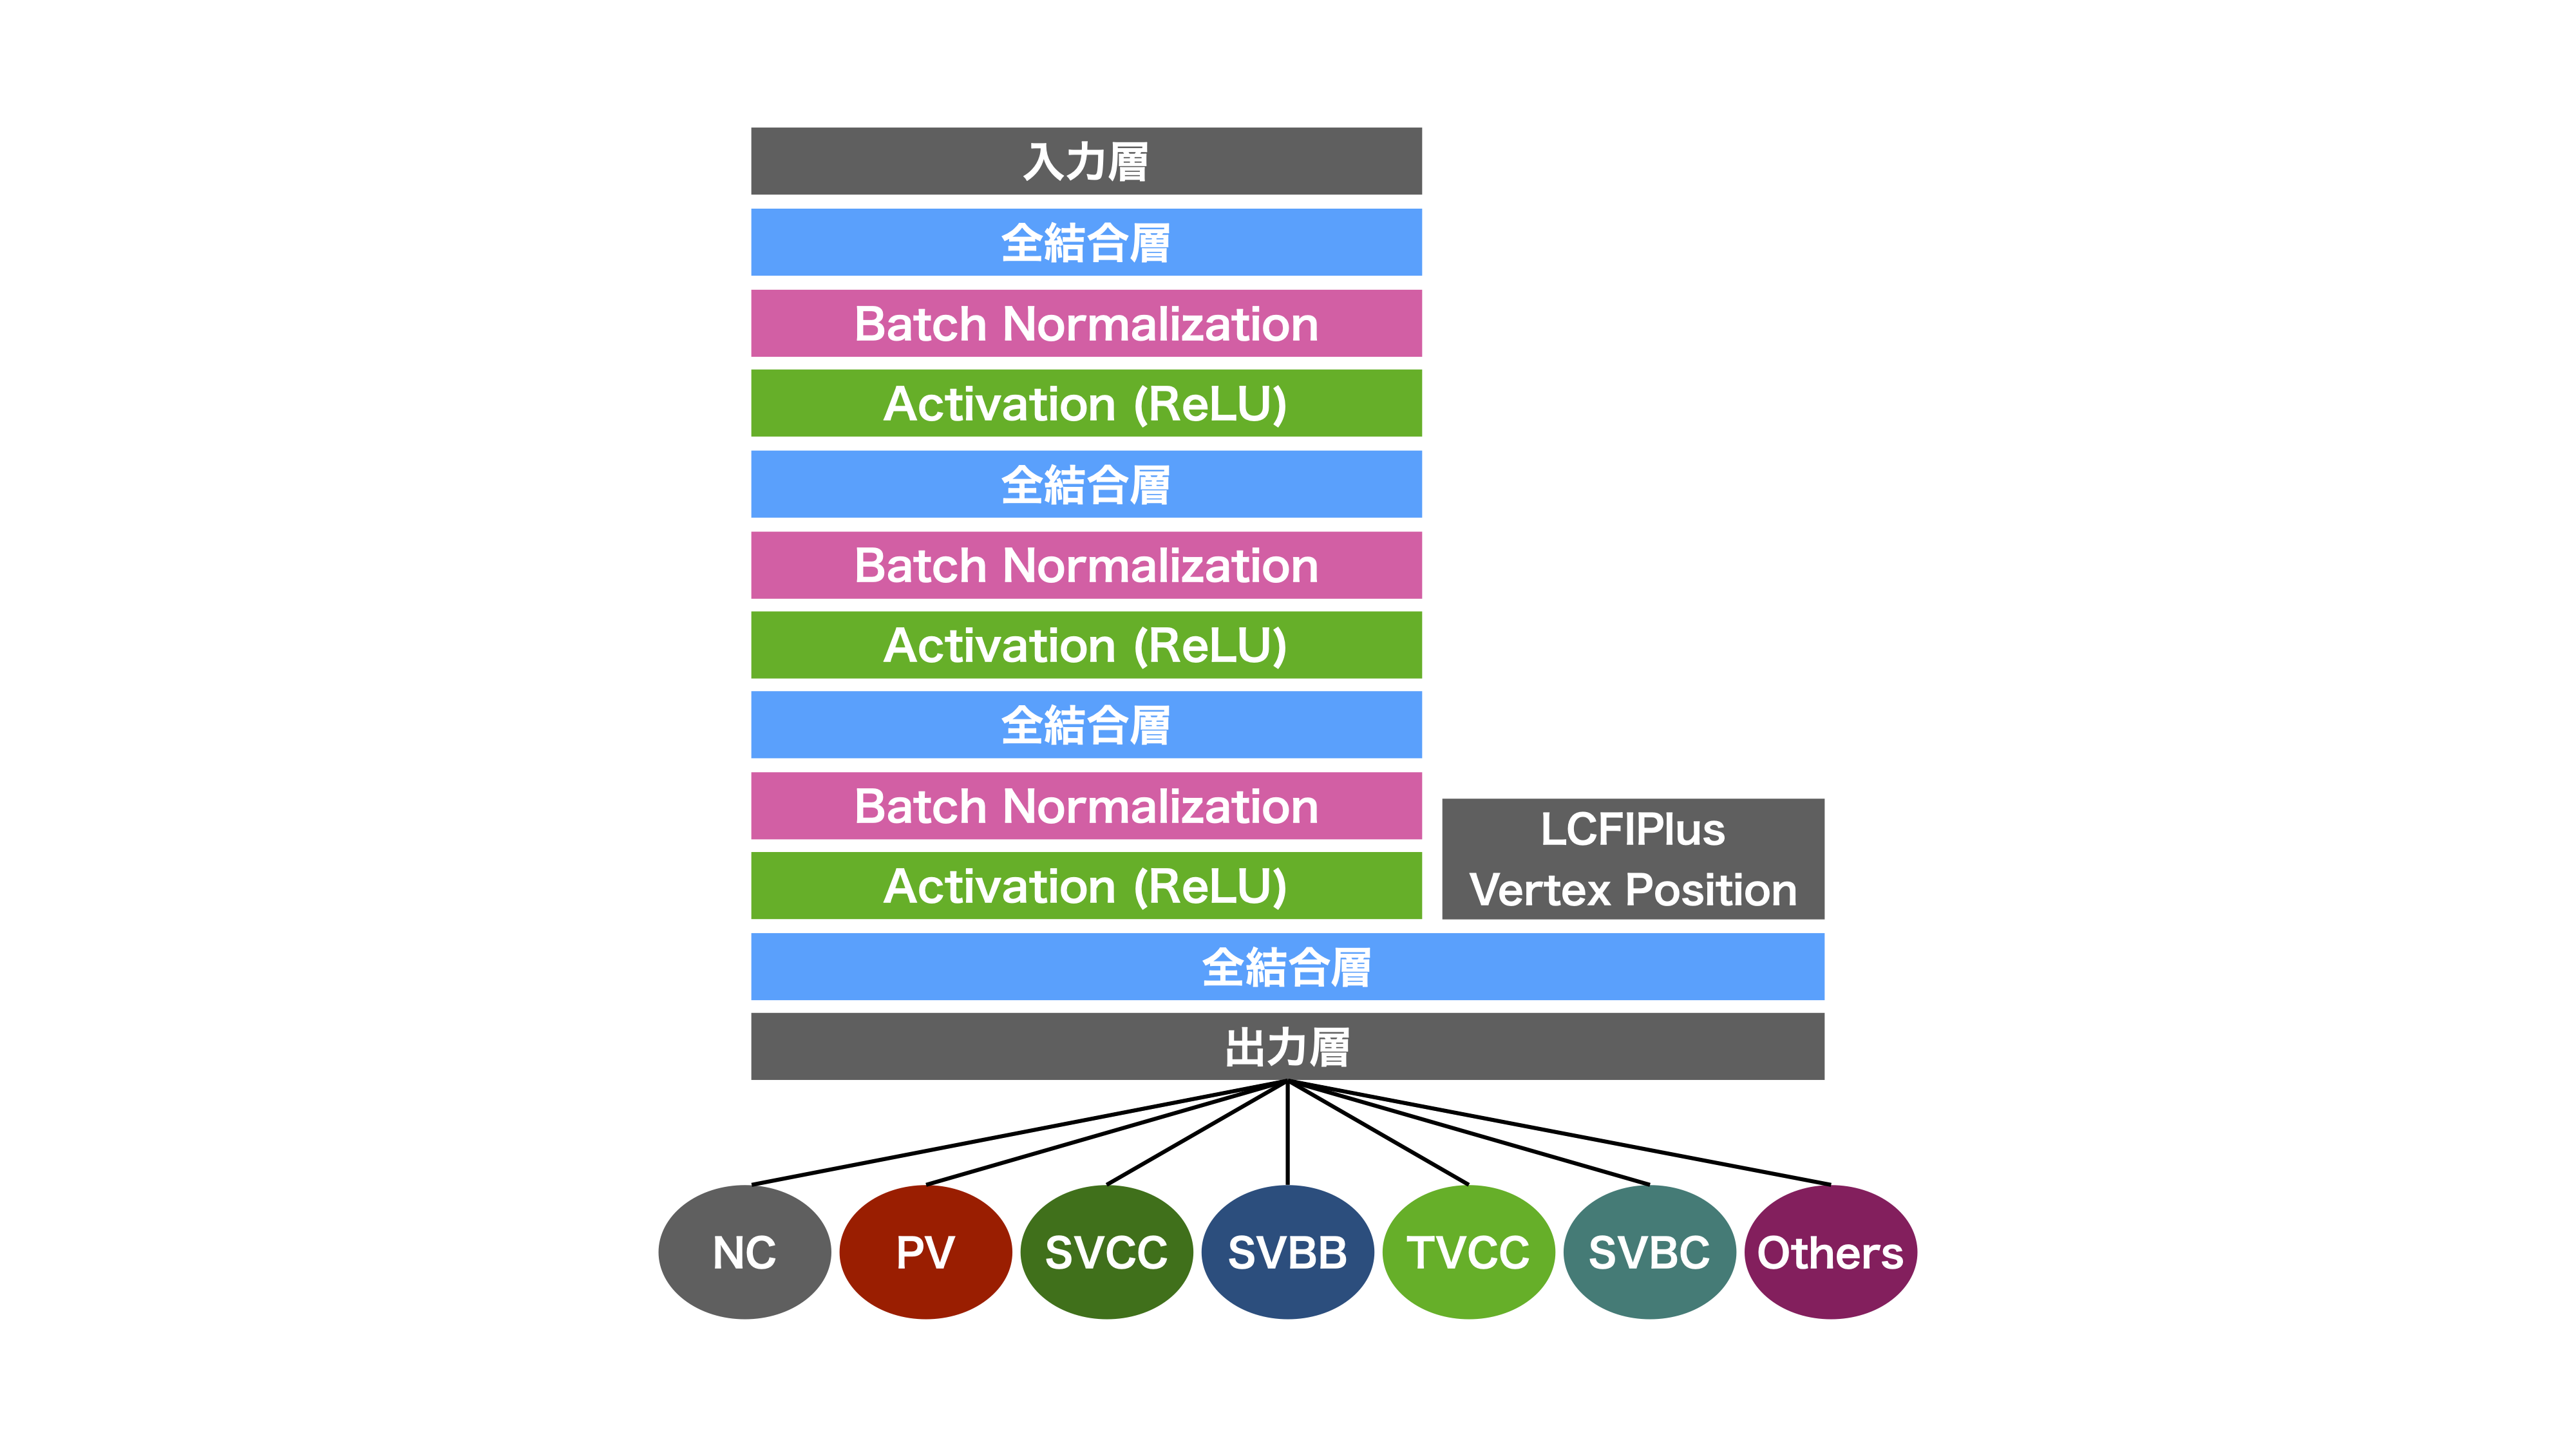
\includegraphics[width=1.0\textwidth, clip]{Figure/3Networks/3-3-3-1PairModelB.png}
    \subcaption{モデルB}
    \label{3-3-3-1PairModelB}
   \end{minipage}
  \end{minipage}
  
  \begin{minipage}{1.0\textwidth}
  \centering
   \begin{minipage}{0.48\textwidth}
   \centering
    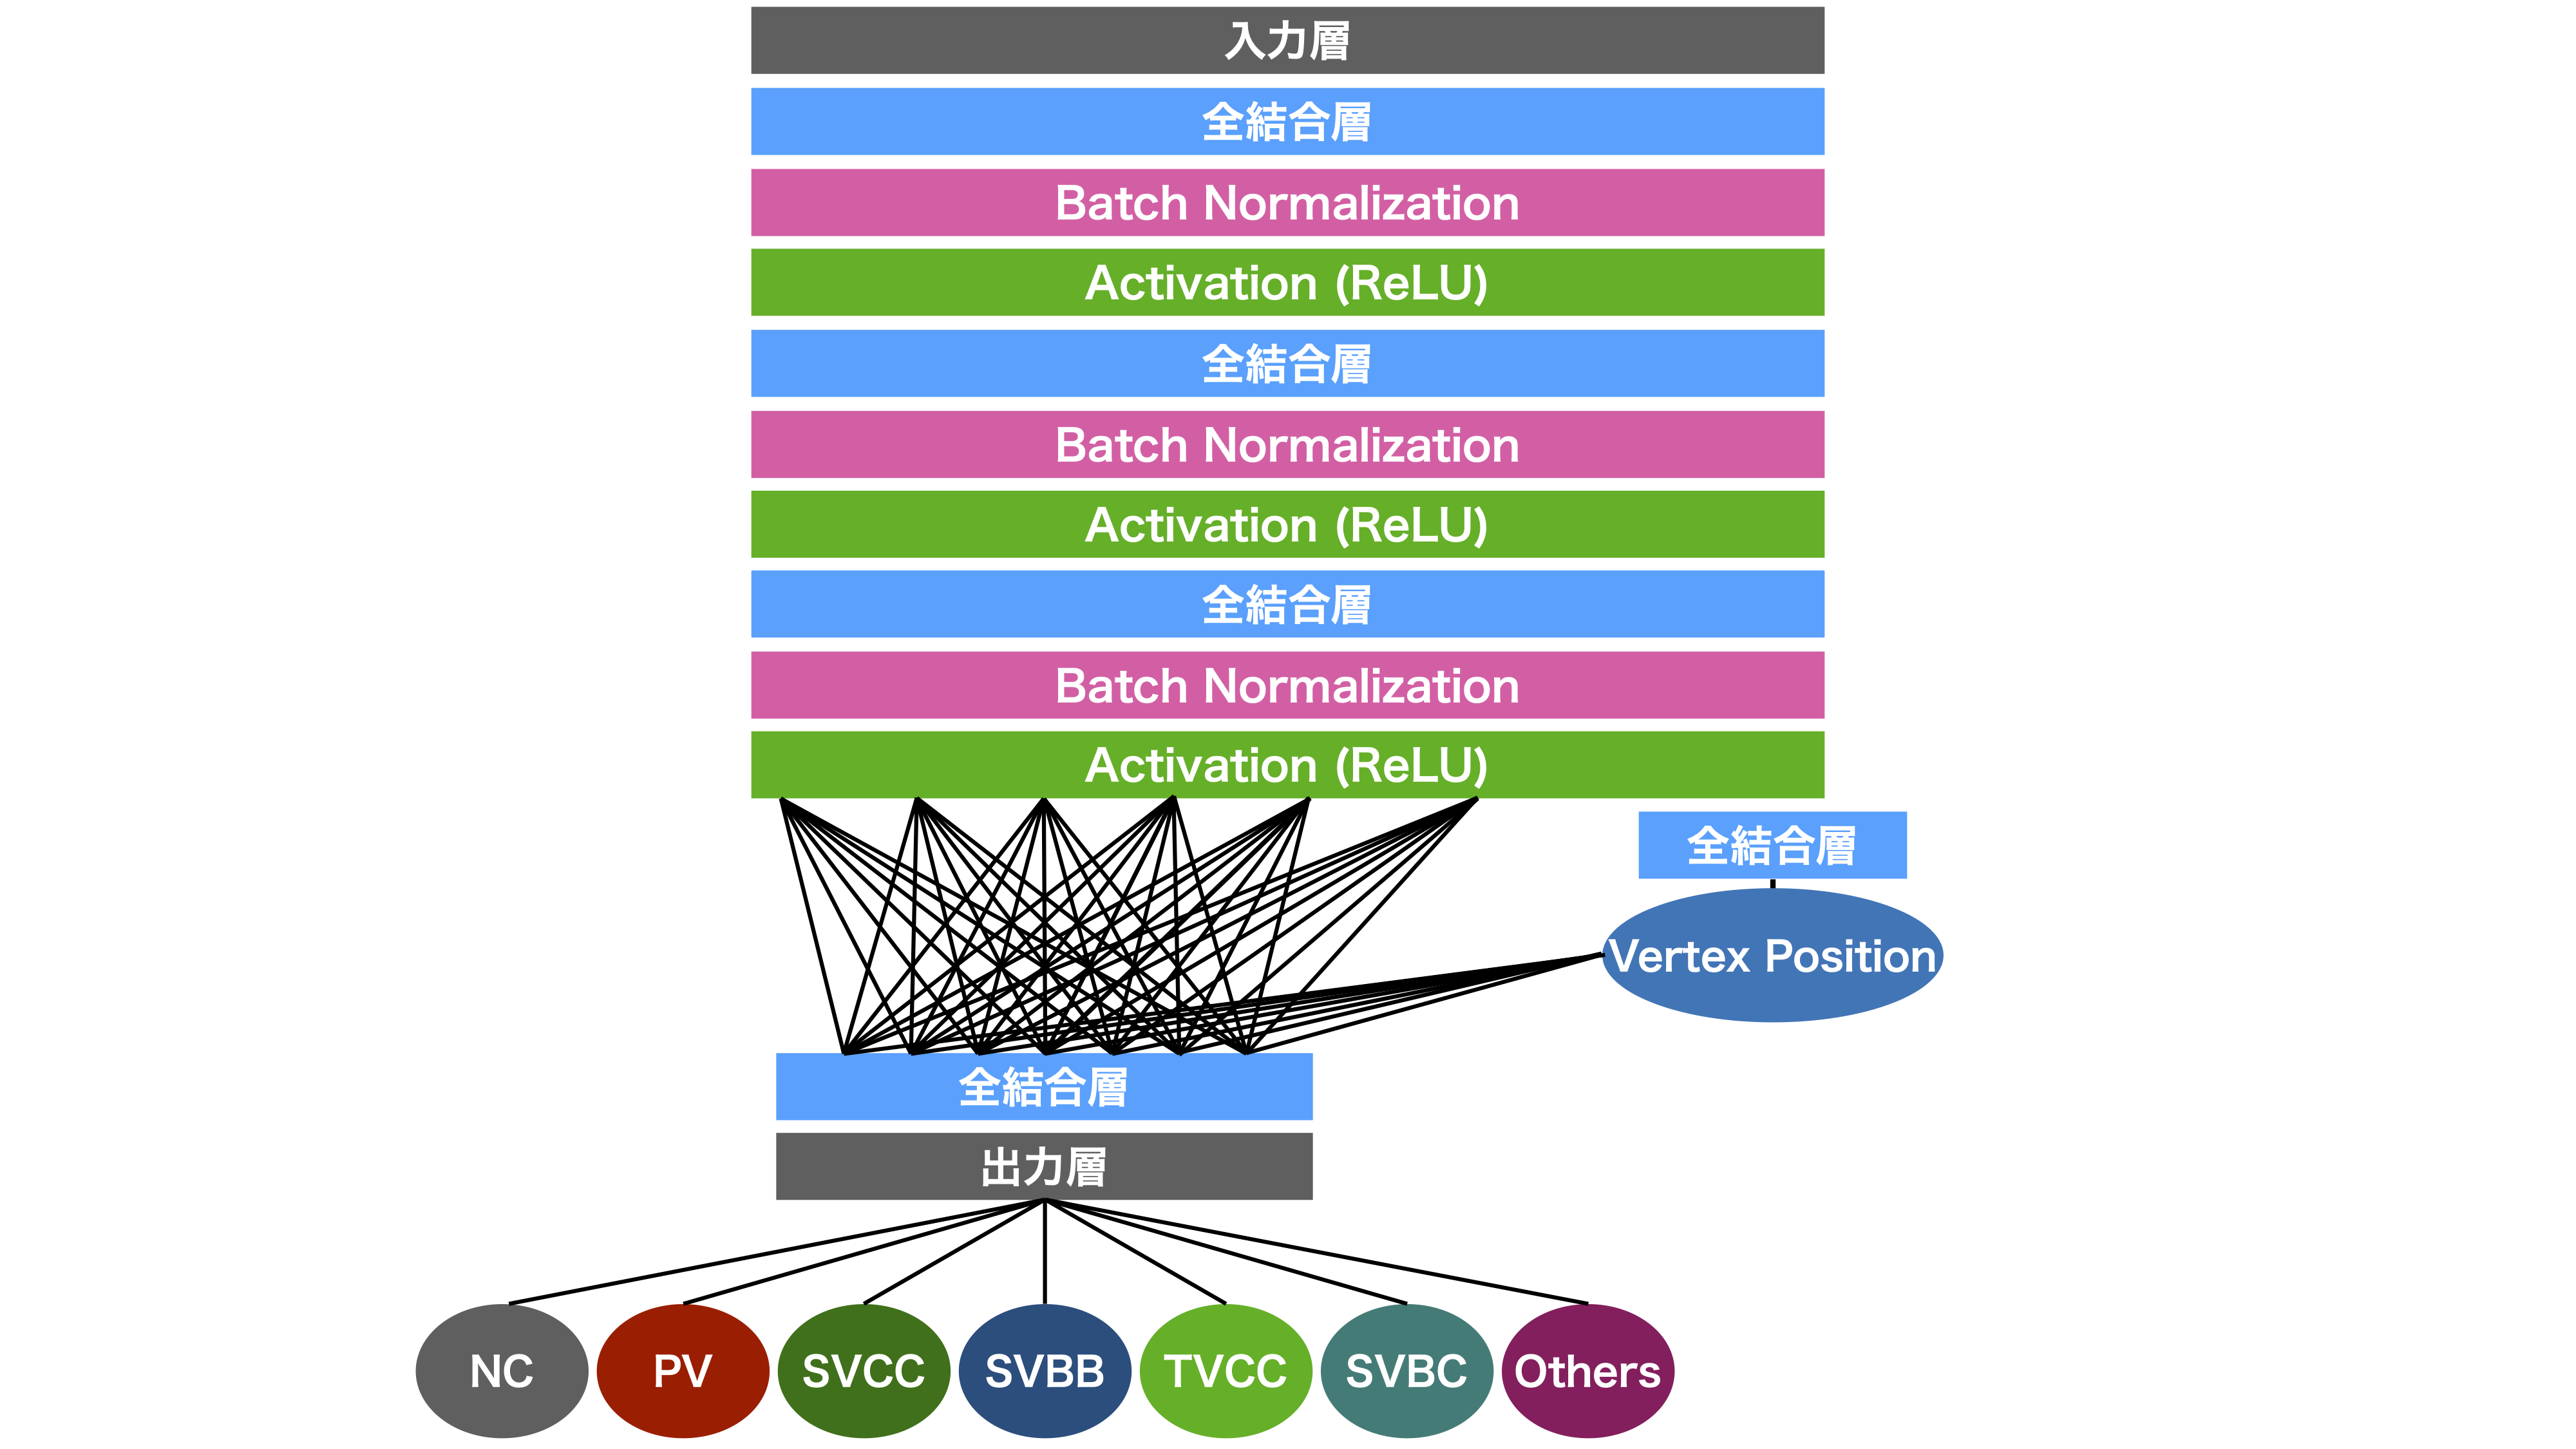
\includegraphics[width=1.0\textwidth, clip]{Figure/3Networks/3-3-3-1PairModelC.png}
    \subcaption{モデルC}
    \label{3-3-3-1PairModelC}
   \end{minipage}
   \begin{minipage}{0.48\textwidth}
   \centering
    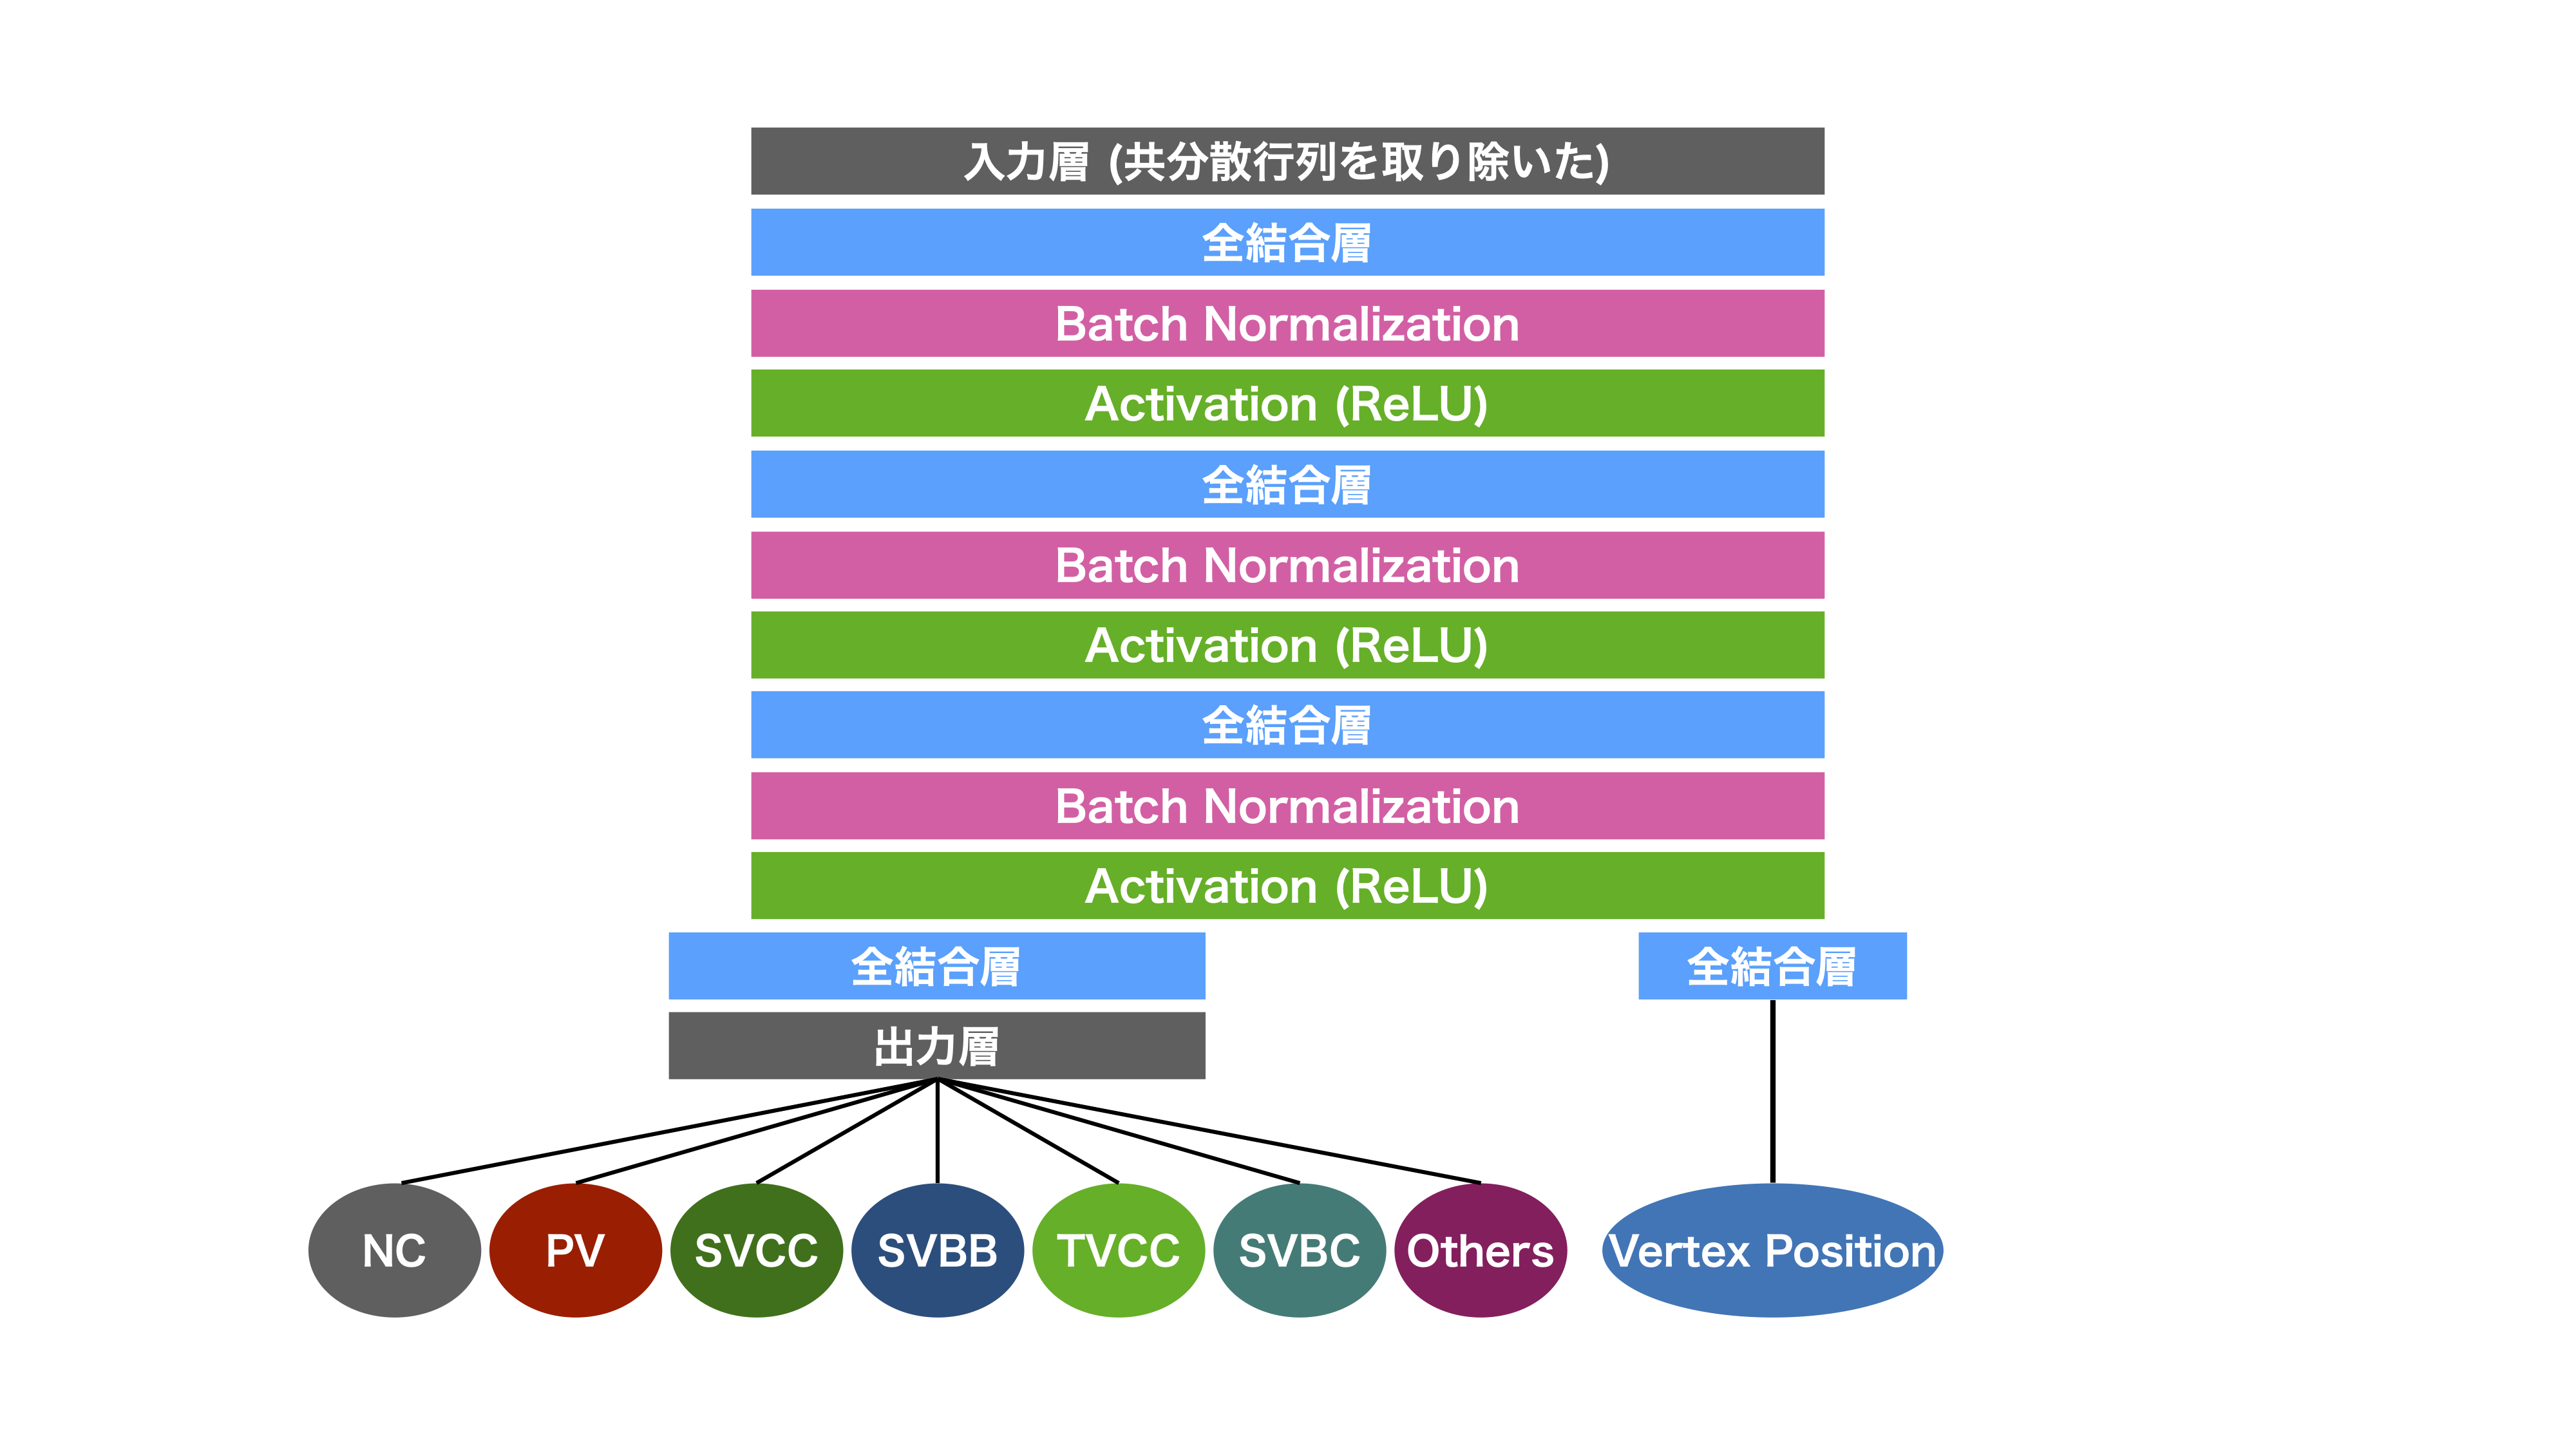
\includegraphics[width=1.0\textwidth, clip]{Figure/3Networks/3-3-3-1PairModelD.png}
    \subcaption{モデルD}
    \label{3-3-3-1PairModelD}
   \end{minipage}
   \end{minipage}
  \caption{評価のための飛跡対についてのネットワーク}
  \label{3-3-3-1PairModels}
 %\end{tabular}
\end{figure}

これらのネットワークの性能は混合行列を用いて評価する。
特にここでは、効率と純度についての混合行列を作成した。
また、出力として崩壊点の位置を予想するネットワークに関しては崩壊点の位置についての損失を用いて評価を行う。

\begin{figure}[htbp]
 \centering
  %\begin{tabular}{cccc}
   \begin{minipage}{1.0\textwidth}
    \centering
    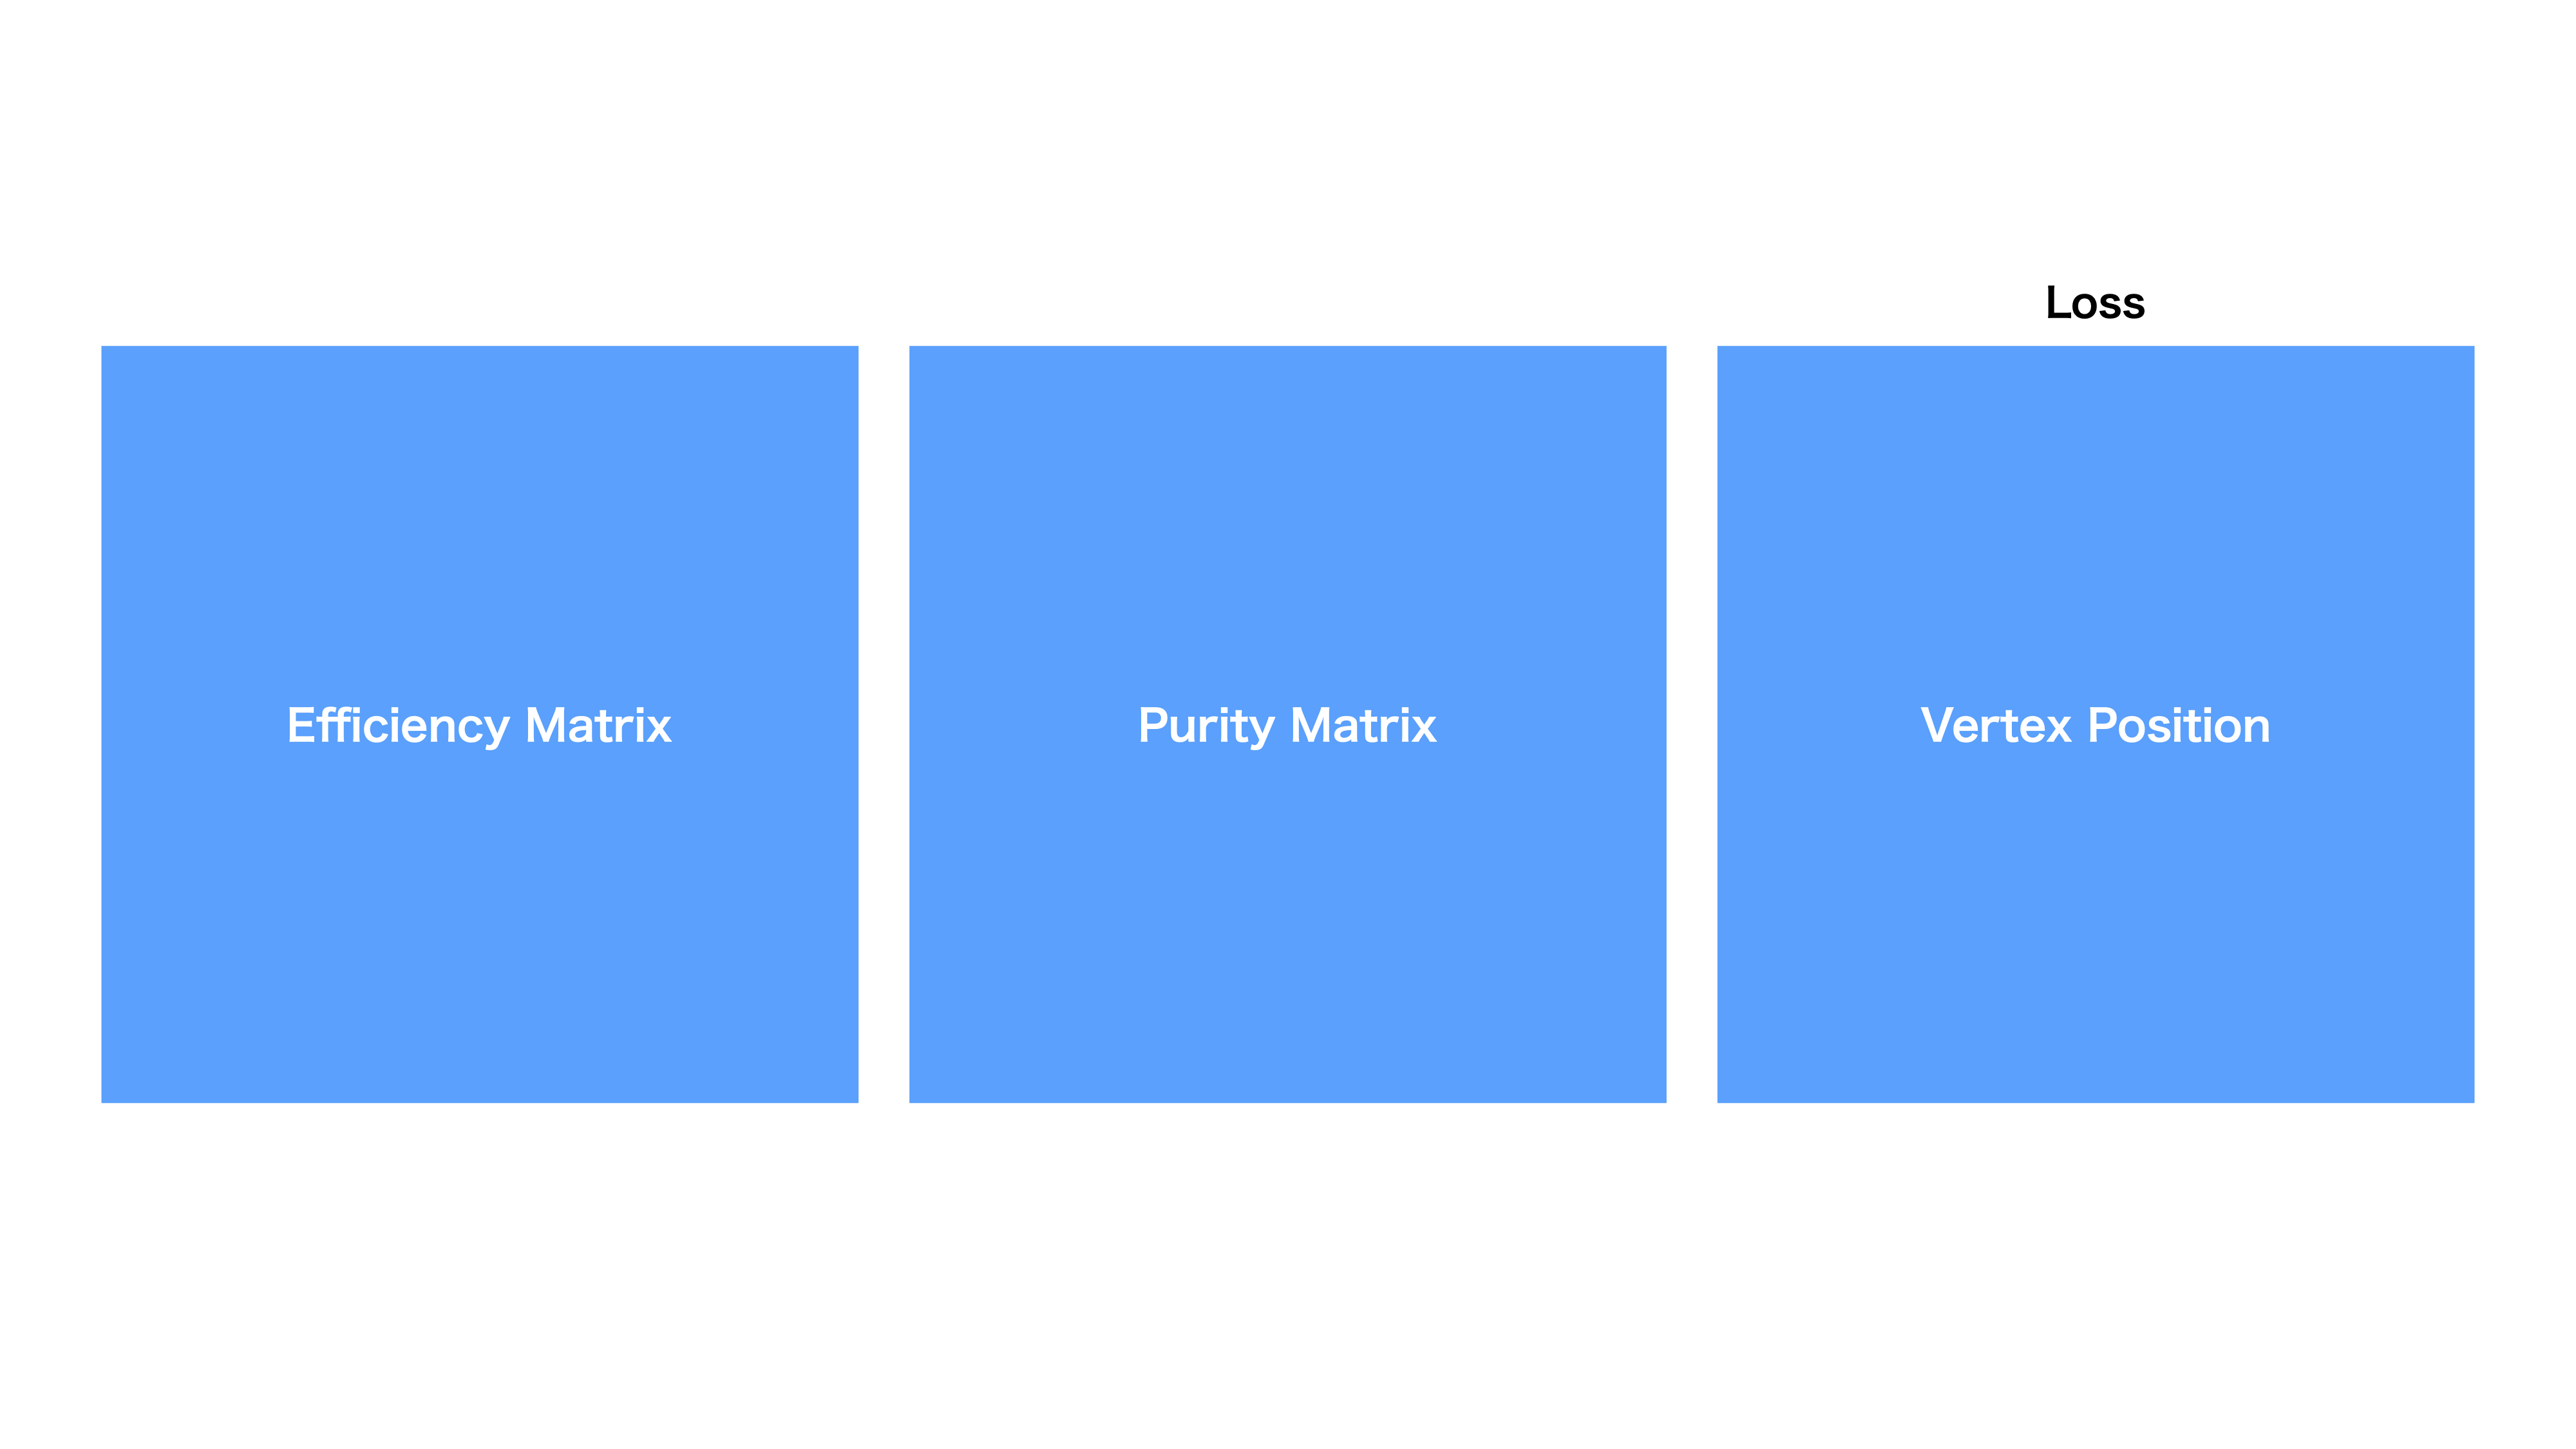
\includegraphics[trim = 0 220 0 220, width=0.9\textwidth, clip]{Figure/3Networks/3-3-3-2ConfusionMatrixA.png}
    \subcaption{モデルAの混合行列と崩壊点の位置}
    \label{3-3-3-2ConfusionMatrixA}
   \end{minipage}

   \begin{minipage}{1.0\textwidth}
   \centering
    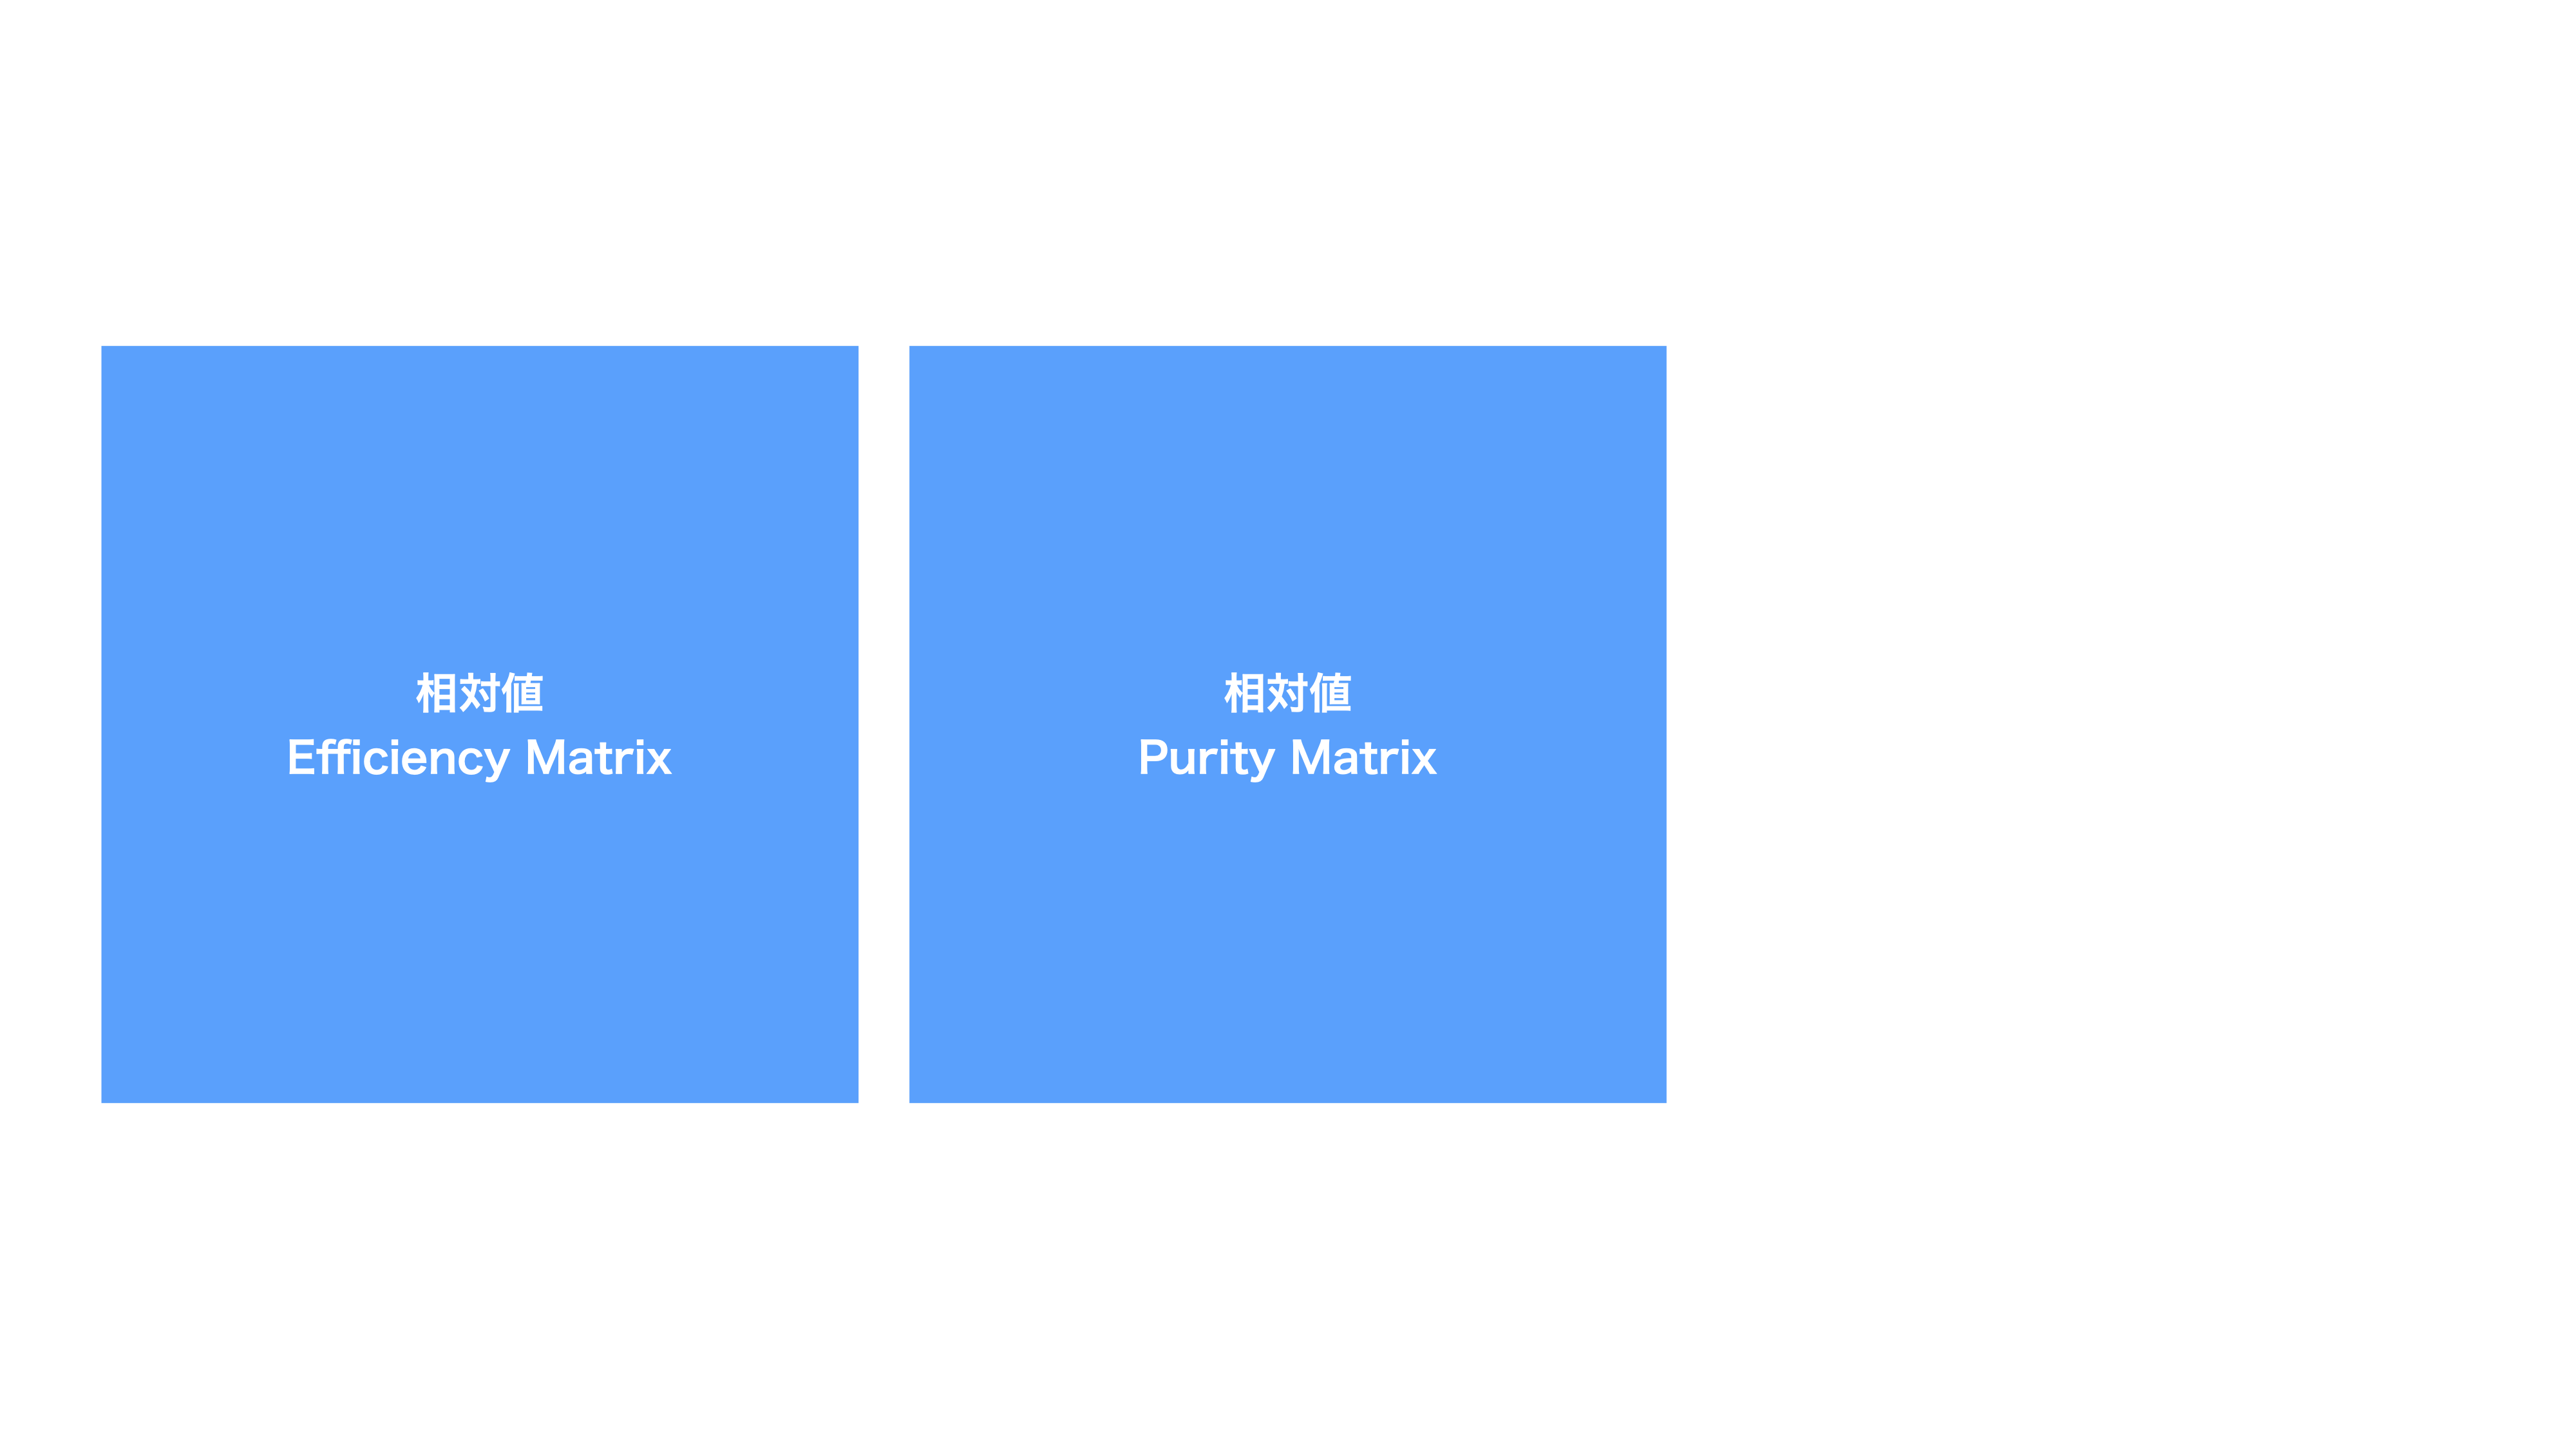
\includegraphics[trim = 0 220 0 220, width=0.9\textwidth, clip]{Figure/3Networks/3-3-3-2ConfusionMatrixB.png}
    \subcaption{モデルBの混合行列の相対値}
    \label{3-3-3-2ConfusionMatrixB}
   \end{minipage}
  
  \begin{minipage}{1.0\textwidth}
   \centering
    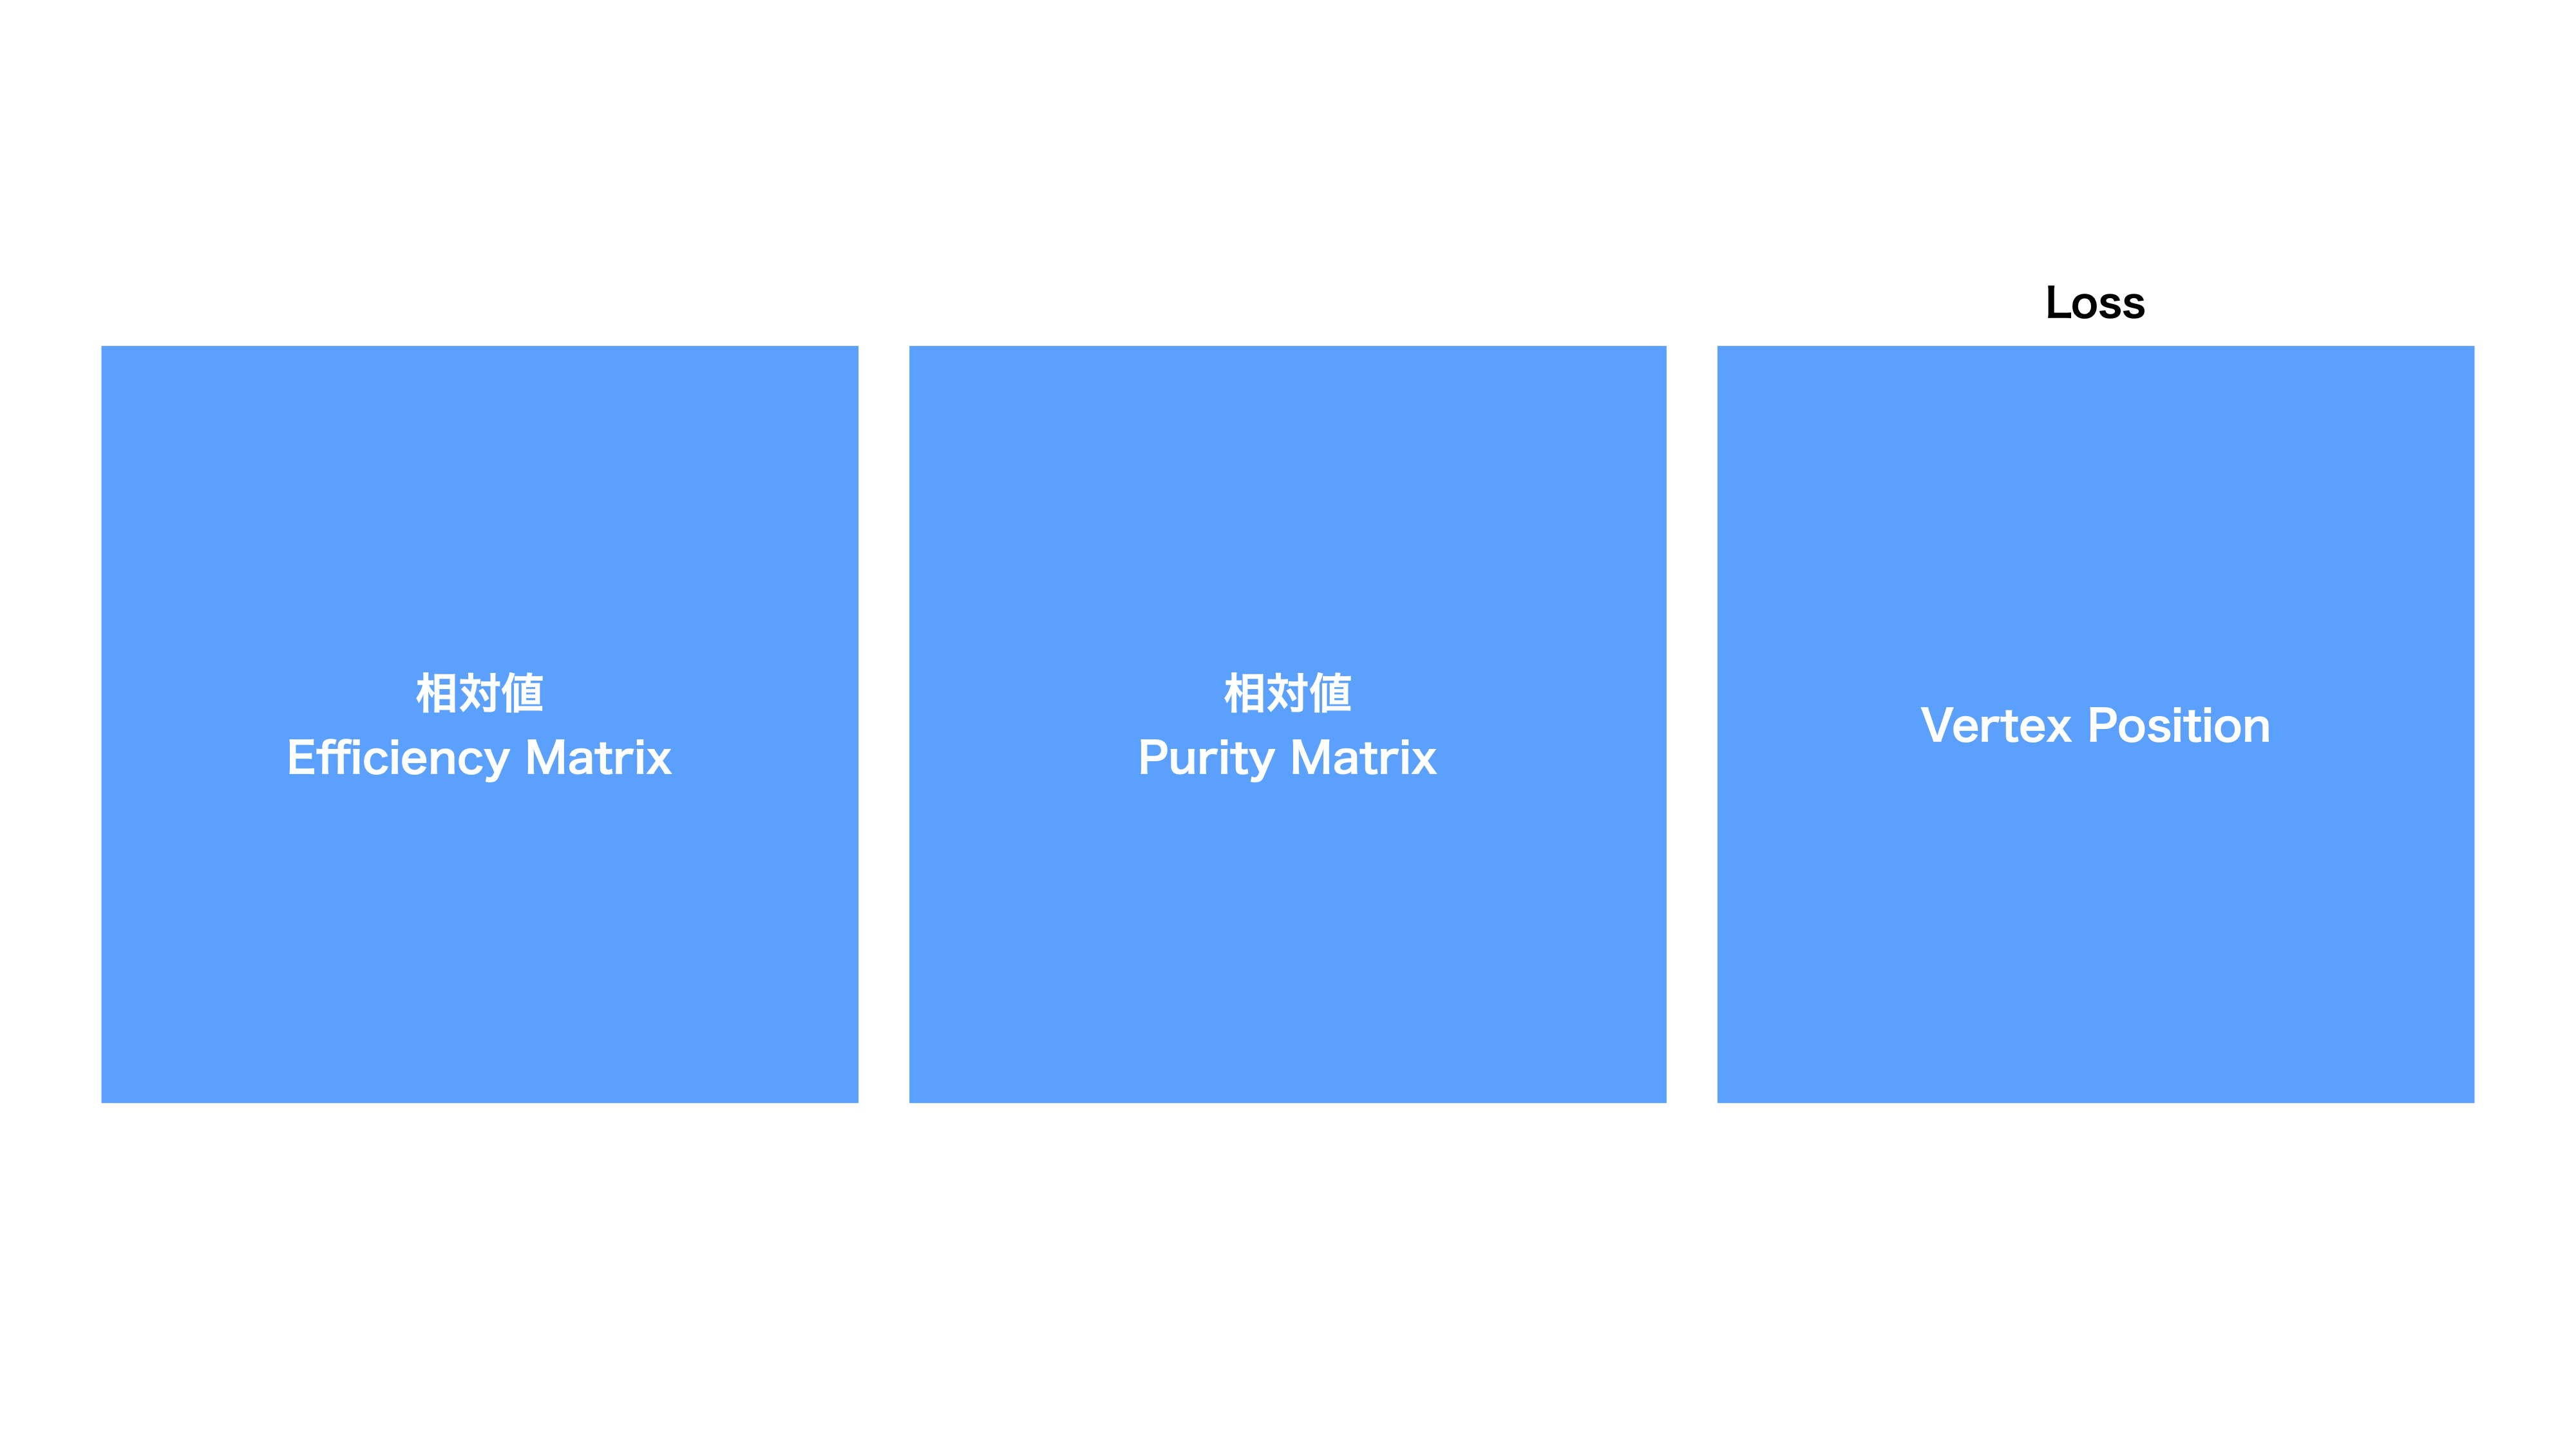
\includegraphics[trim = 0 220 0 220, width=0.9\textwidth, clip]{Figure/3Networks/3-3-3-2ConfusionMatrixC.png}
    \subcaption{モデルCの混合行列の相対値と崩壊点の位置}
    \label{3-3-3-2ConfusionMatrixC}
   \end{minipage}
   
   \begin{minipage}{1.0\textwidth}
   \centering
    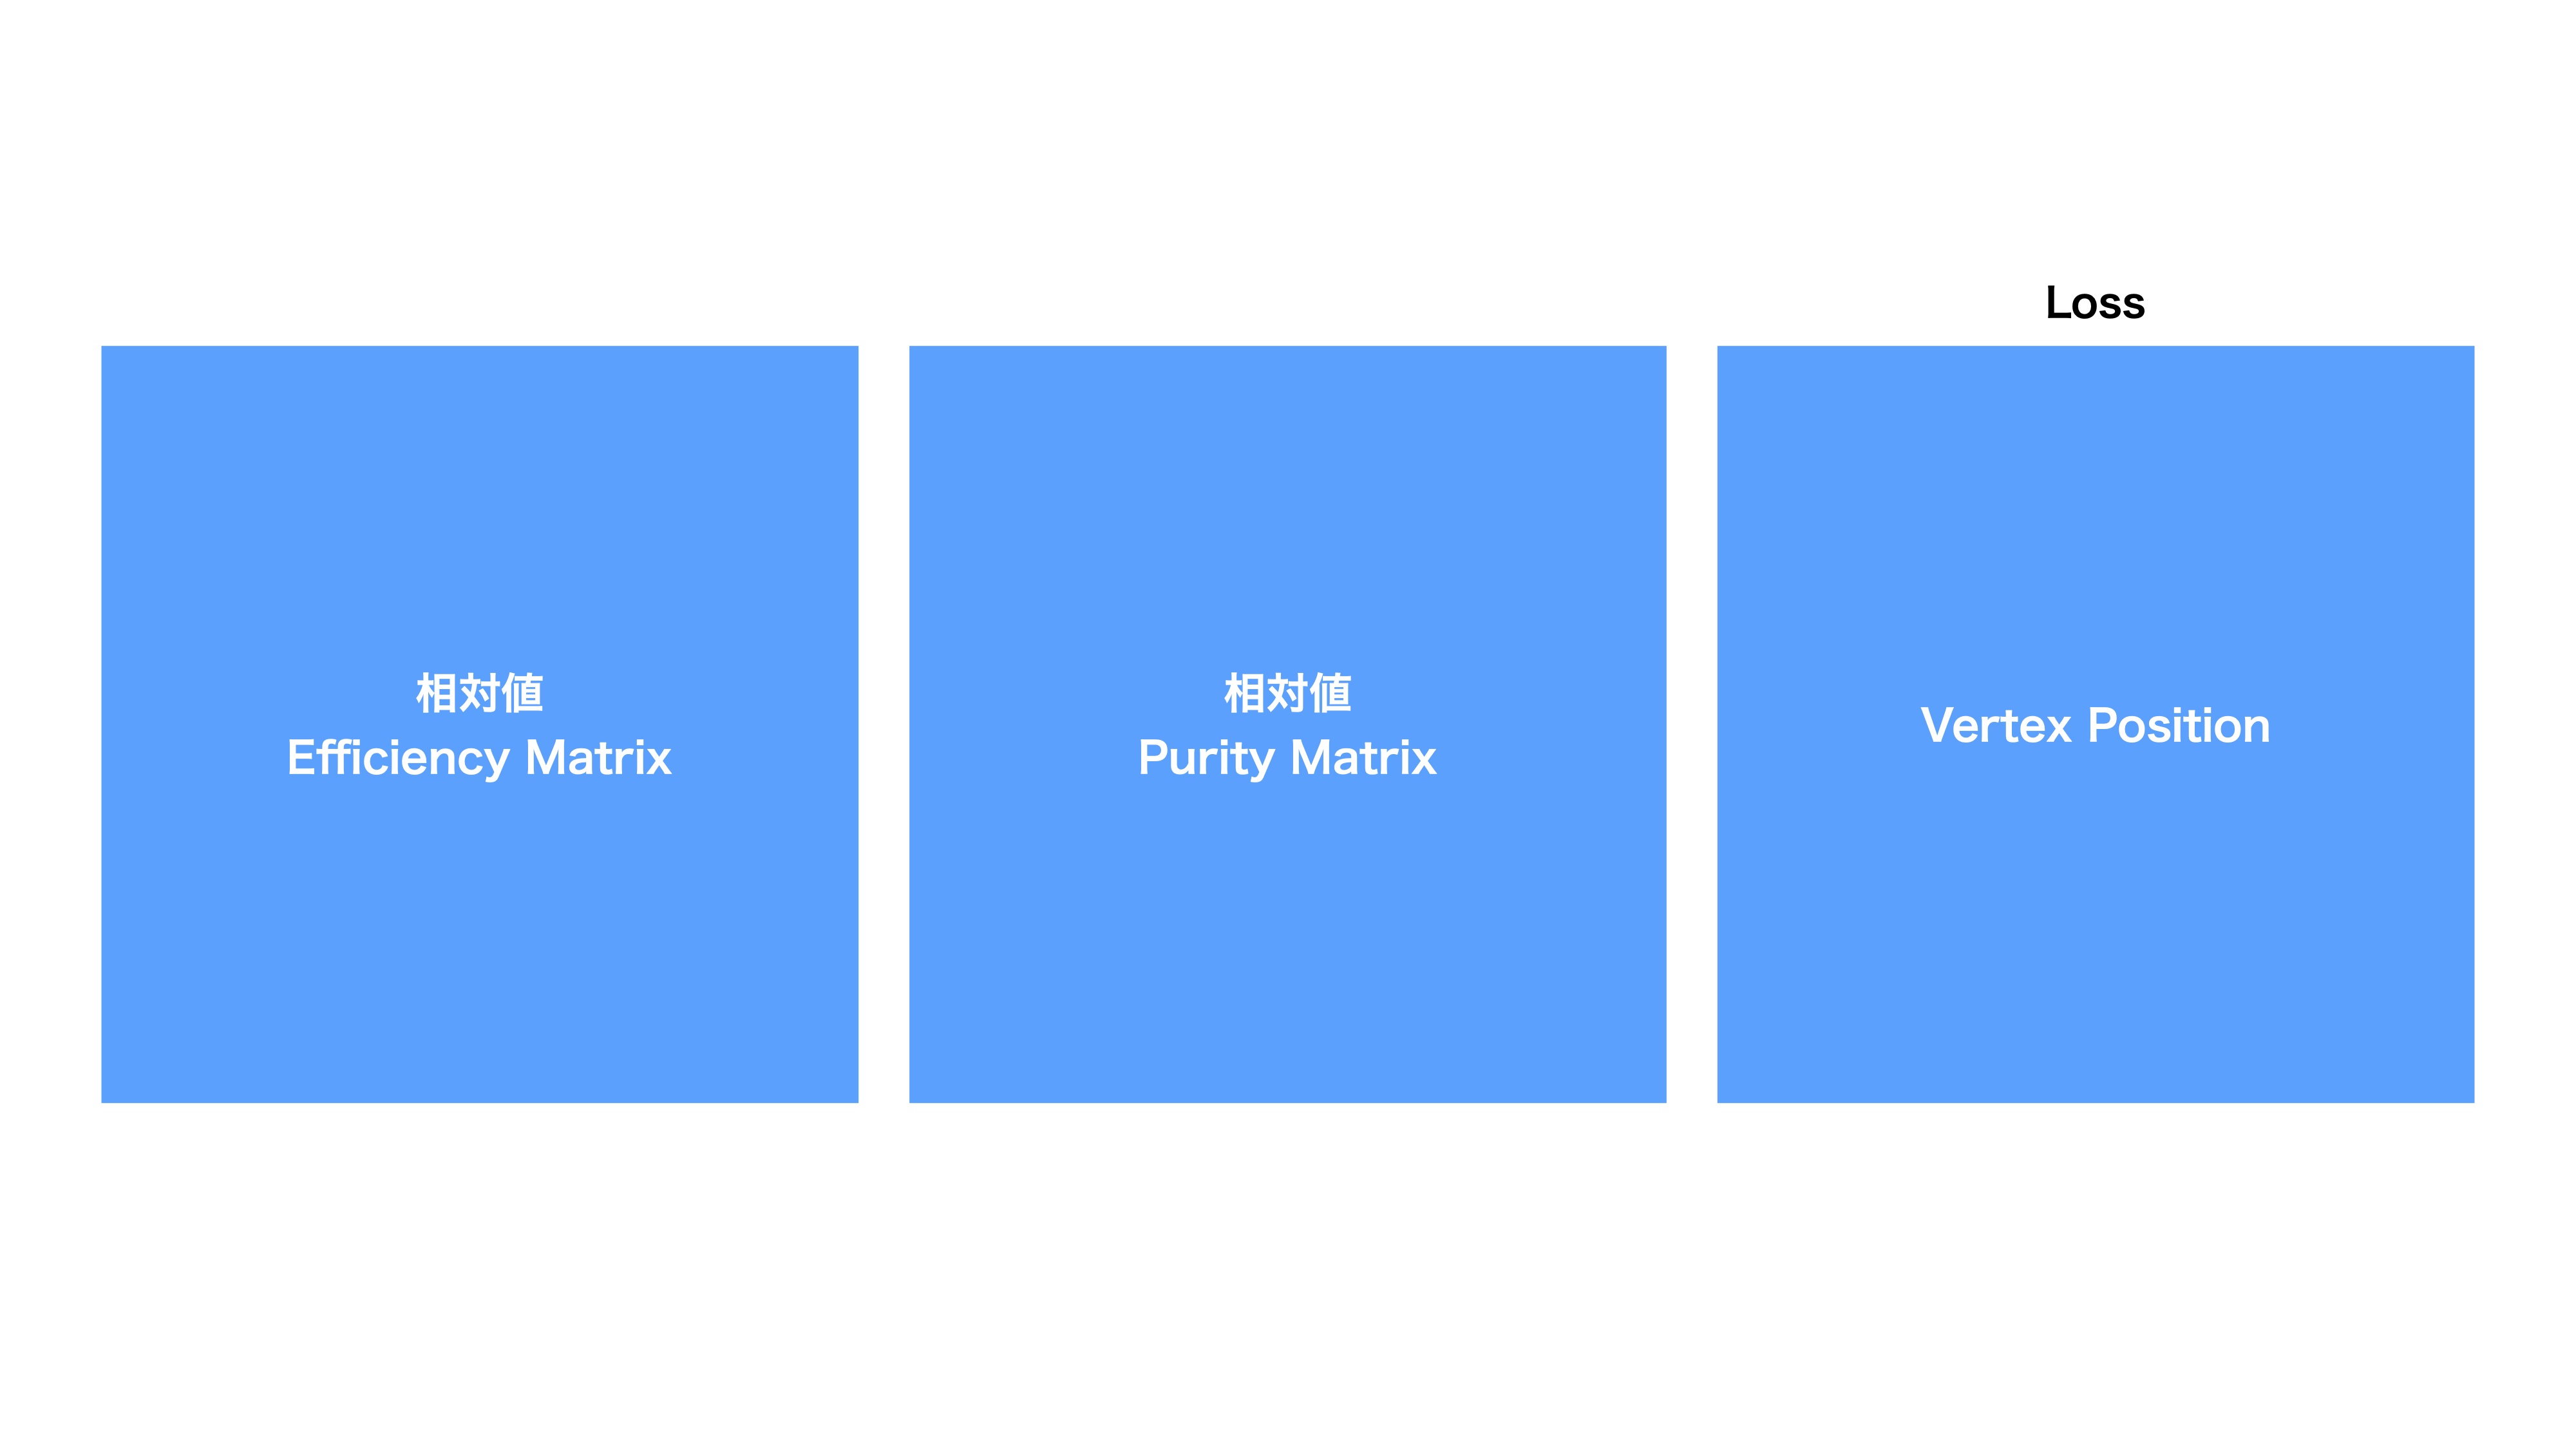
\includegraphics[trim = 0 220 0 220, width=0.9\textwidth, clip]{Figure/3Networks/3-3-3-2ConfusionMatrixD.png}
    \subcaption{モデルDの混合行列の相対値と崩壊点の位置}
    \label{3-3-3-2ConfusionMatrixD}
   \end{minipage}
  \caption{各ネットワークの混合行列と崩壊点の位置}
  \label{3-3-3-2ConfusionMatrices}
 %\end{tabular}
\end{figure}

ROCカーブ\\

\begin{figure}[htbp]
 \centering
 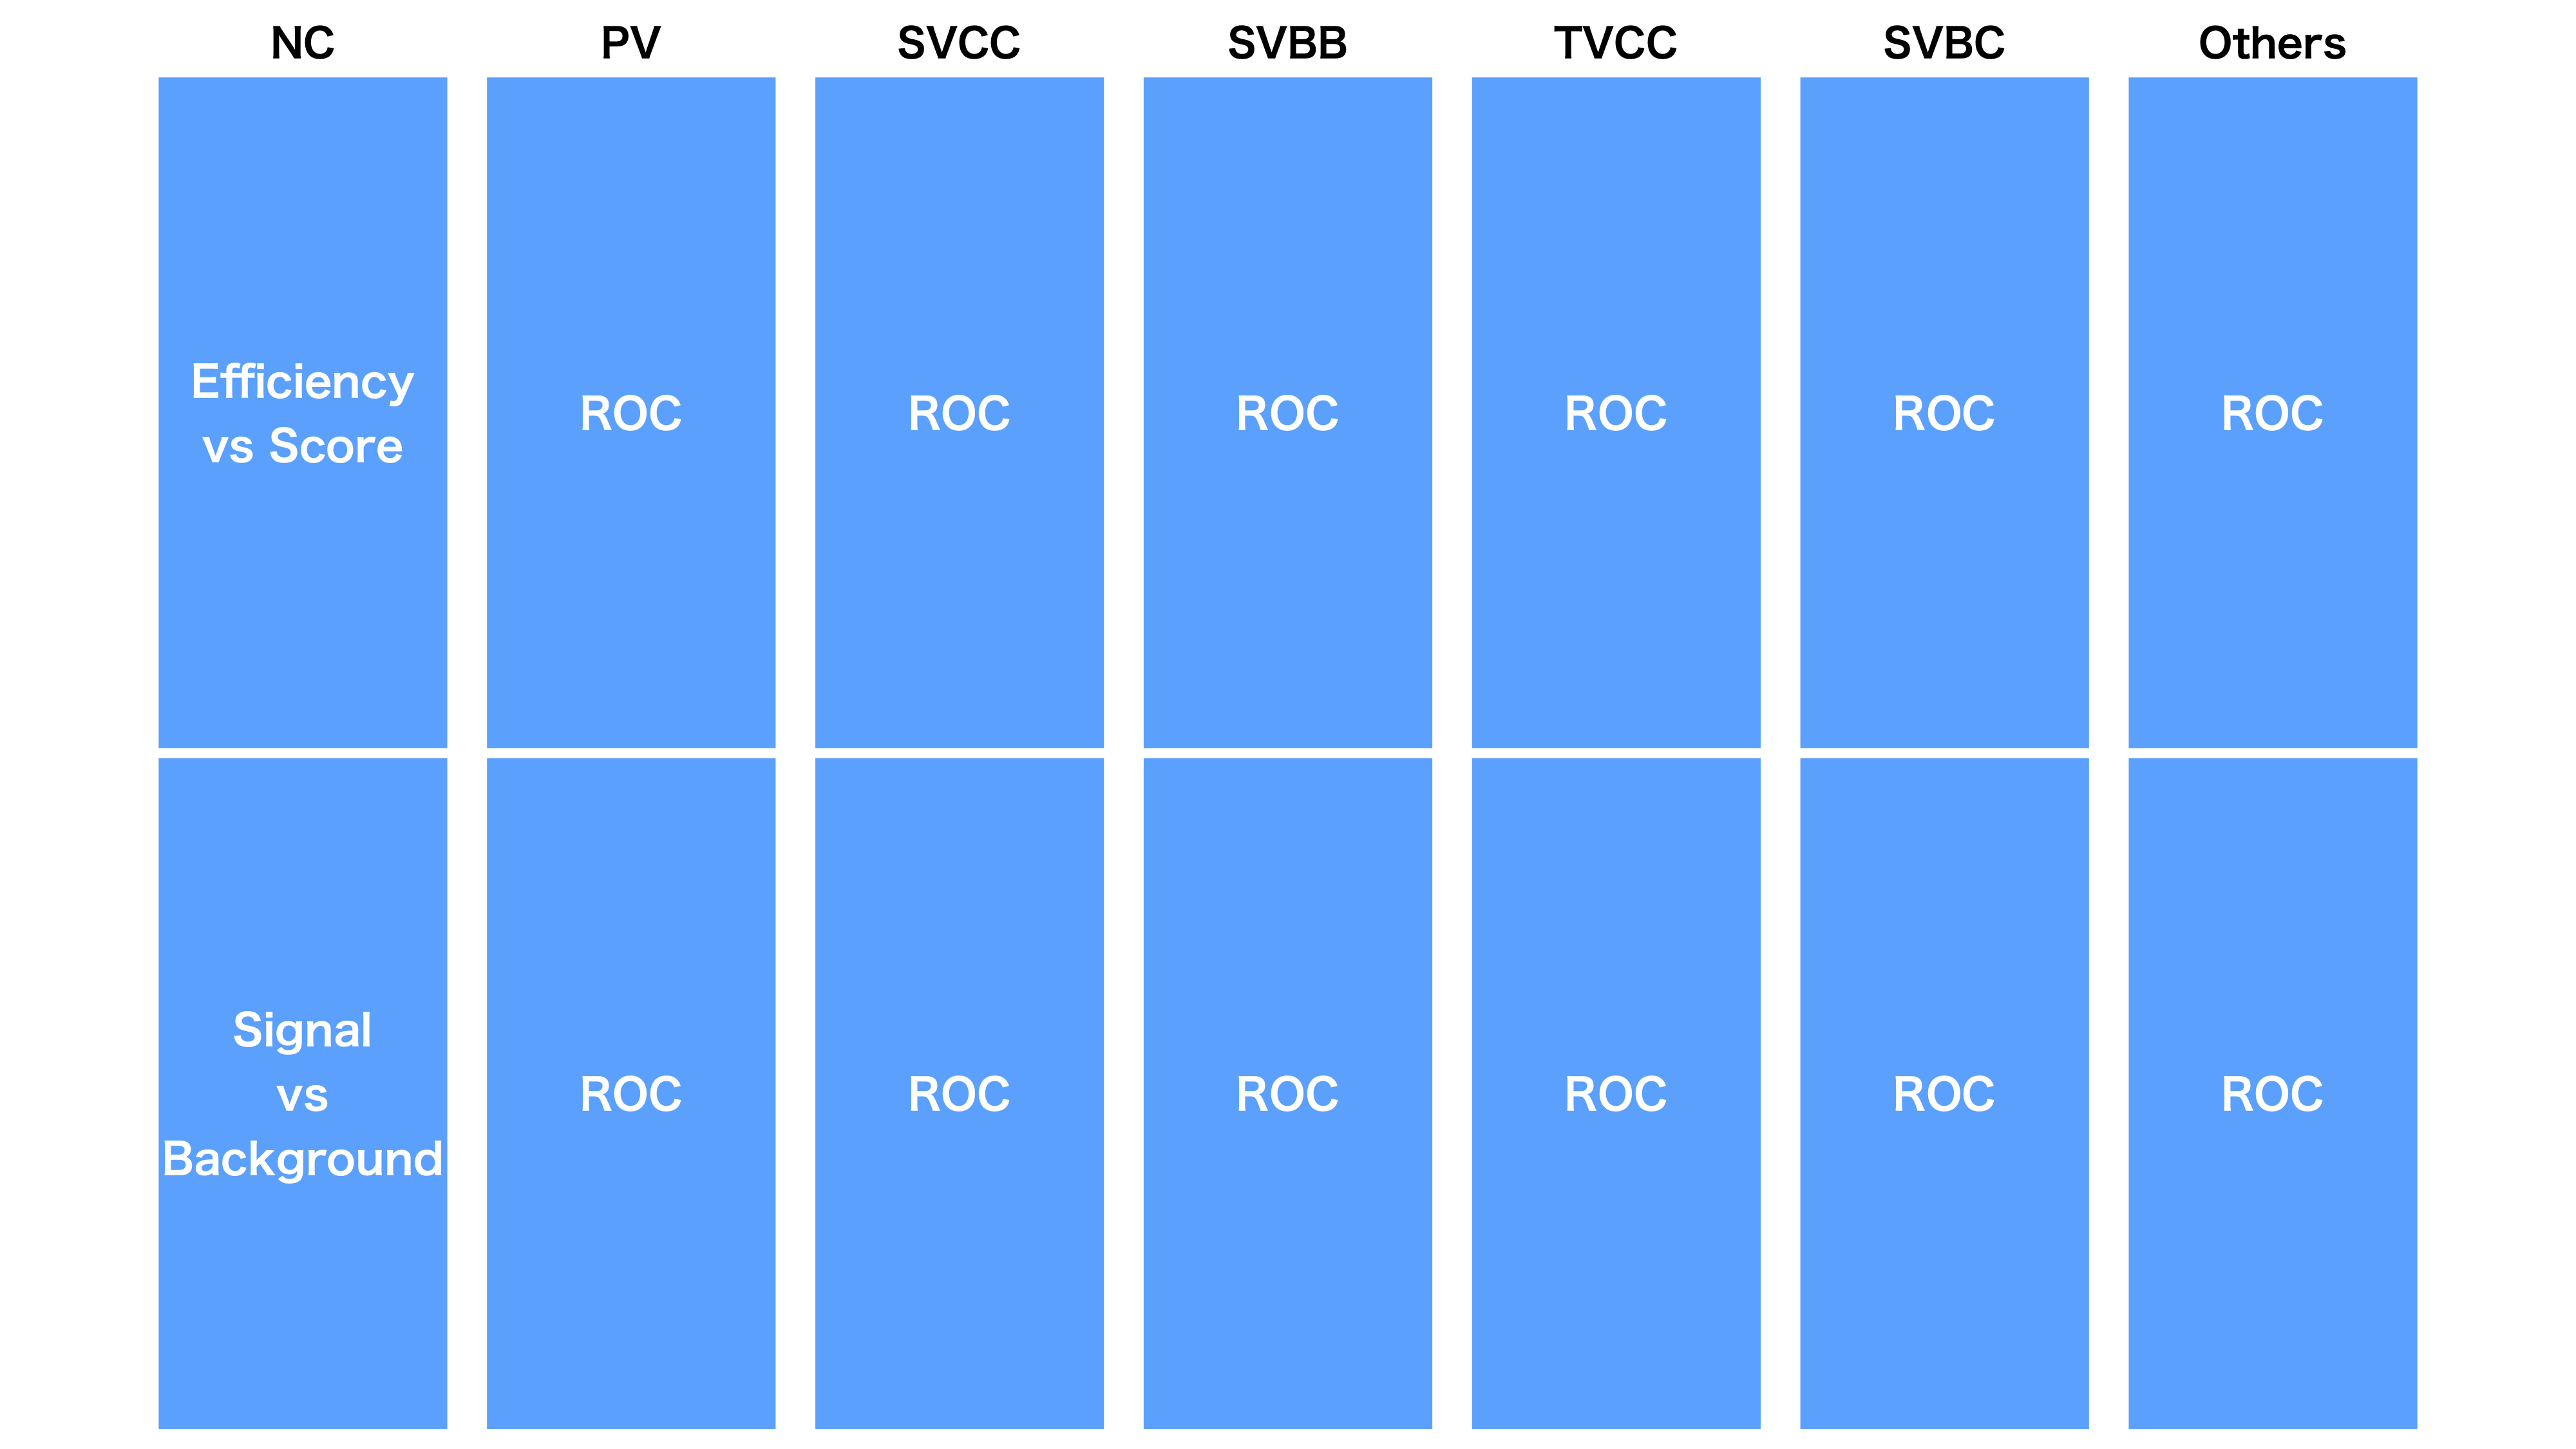
\includegraphics[width=1.0\textwidth]{Figure/3Networks/3-3-3-3ROCCurve.png}
 \caption{飛跡対についてのネットワークに関するROC曲線}
 \label{3-3-3-3ROCCurve}
\end{figure}



%%%%%%%%%%%%%%%%%%%%%%%%%%%%%%%%%%%%%%%%%%%%%%%%%%%%%%%%%%%%%%%%%%%%%%%%%%%%%%%%%%%%%%%%%%%%%%%%%%%%%
\section{任意の数の飛跡についてのネットワーク} \label{Net:VertexLSTM}

ここでは\ref{Net:forVertexFinderwithDL}節で紹介した二つのネットワークの内、任意の数の飛跡のためのネットワークについて述べる。
基本的には前節の飛跡対についてのネットワークと同様の手順での解説を行うが、この任意の数の飛跡についてのネットワークは、既存のネットワーク構造にはない独自のネットワークで構築している。
これは本研究におけるデータの特殊性や問題解決のための最適なネットワークを考慮した結果である。
このようなネットワークの詳細な構造については\ref{Net:VLSTM:DetailedStructureofVLSTM}項で述べる。


%%%%%%%%%%%%%%%%%%%%%%%%%%%%%%%%%%%%%%%%%%%%%%%%%%%%%%%%%%%%%%%%%%%%%%%%
\subsection{ネットワークの構造} \label{Net:VLSTM:StructureofVLSTM}

任意の数の飛跡についてのネットワークではリカレントニューラルネットワークの技術を採用している。
ただし、飛跡は本質的に順序を持っておらず、系列データではない為、リカレントニューラルネットワークをそのまま用いることはデータの性質に合わない。
この為私は、リカレントニューラルネットワークの一つであるLSTMを拡張し、新しい独自のリカレントニューラルネットワークの構造を構築した。
この独自のネットワーク構造については、次項\ref{Net:VLSTM:DetailedStructureofVLSTM}にて解説する。
ここでは、より大きな枠組みとしてのネットワークの構造について述べる。

図\ref{3-4-1-1SimpleVLSTM}は、リカレントニューラルネットワークを用いた最も簡単な崩壊点生成を表現したものである。
ここで、左から崩壊点の種である飛跡対が入力されている。
実際には全結合層を通し、リカレントニューラルネットワークの初期状態としている。
この初期状態は、リカレントニューラルネットワーク内の重みと共に全結合層が学習される為、学習可能な初期状態 (Trainable (Learnable) Initial State) となっている。
また、飛跡は下から一本ずつ入力され、1事象分の全ての飛跡が使用されるが、リカレントニューラルネットワークである為、系列として扱う飛跡の本数は任意である。
したがって、ある崩壊点のタネに対して、任意の数の飛跡が結合しているか否かを分類することができる。

\begin{figure}[htbp]
 \centering
 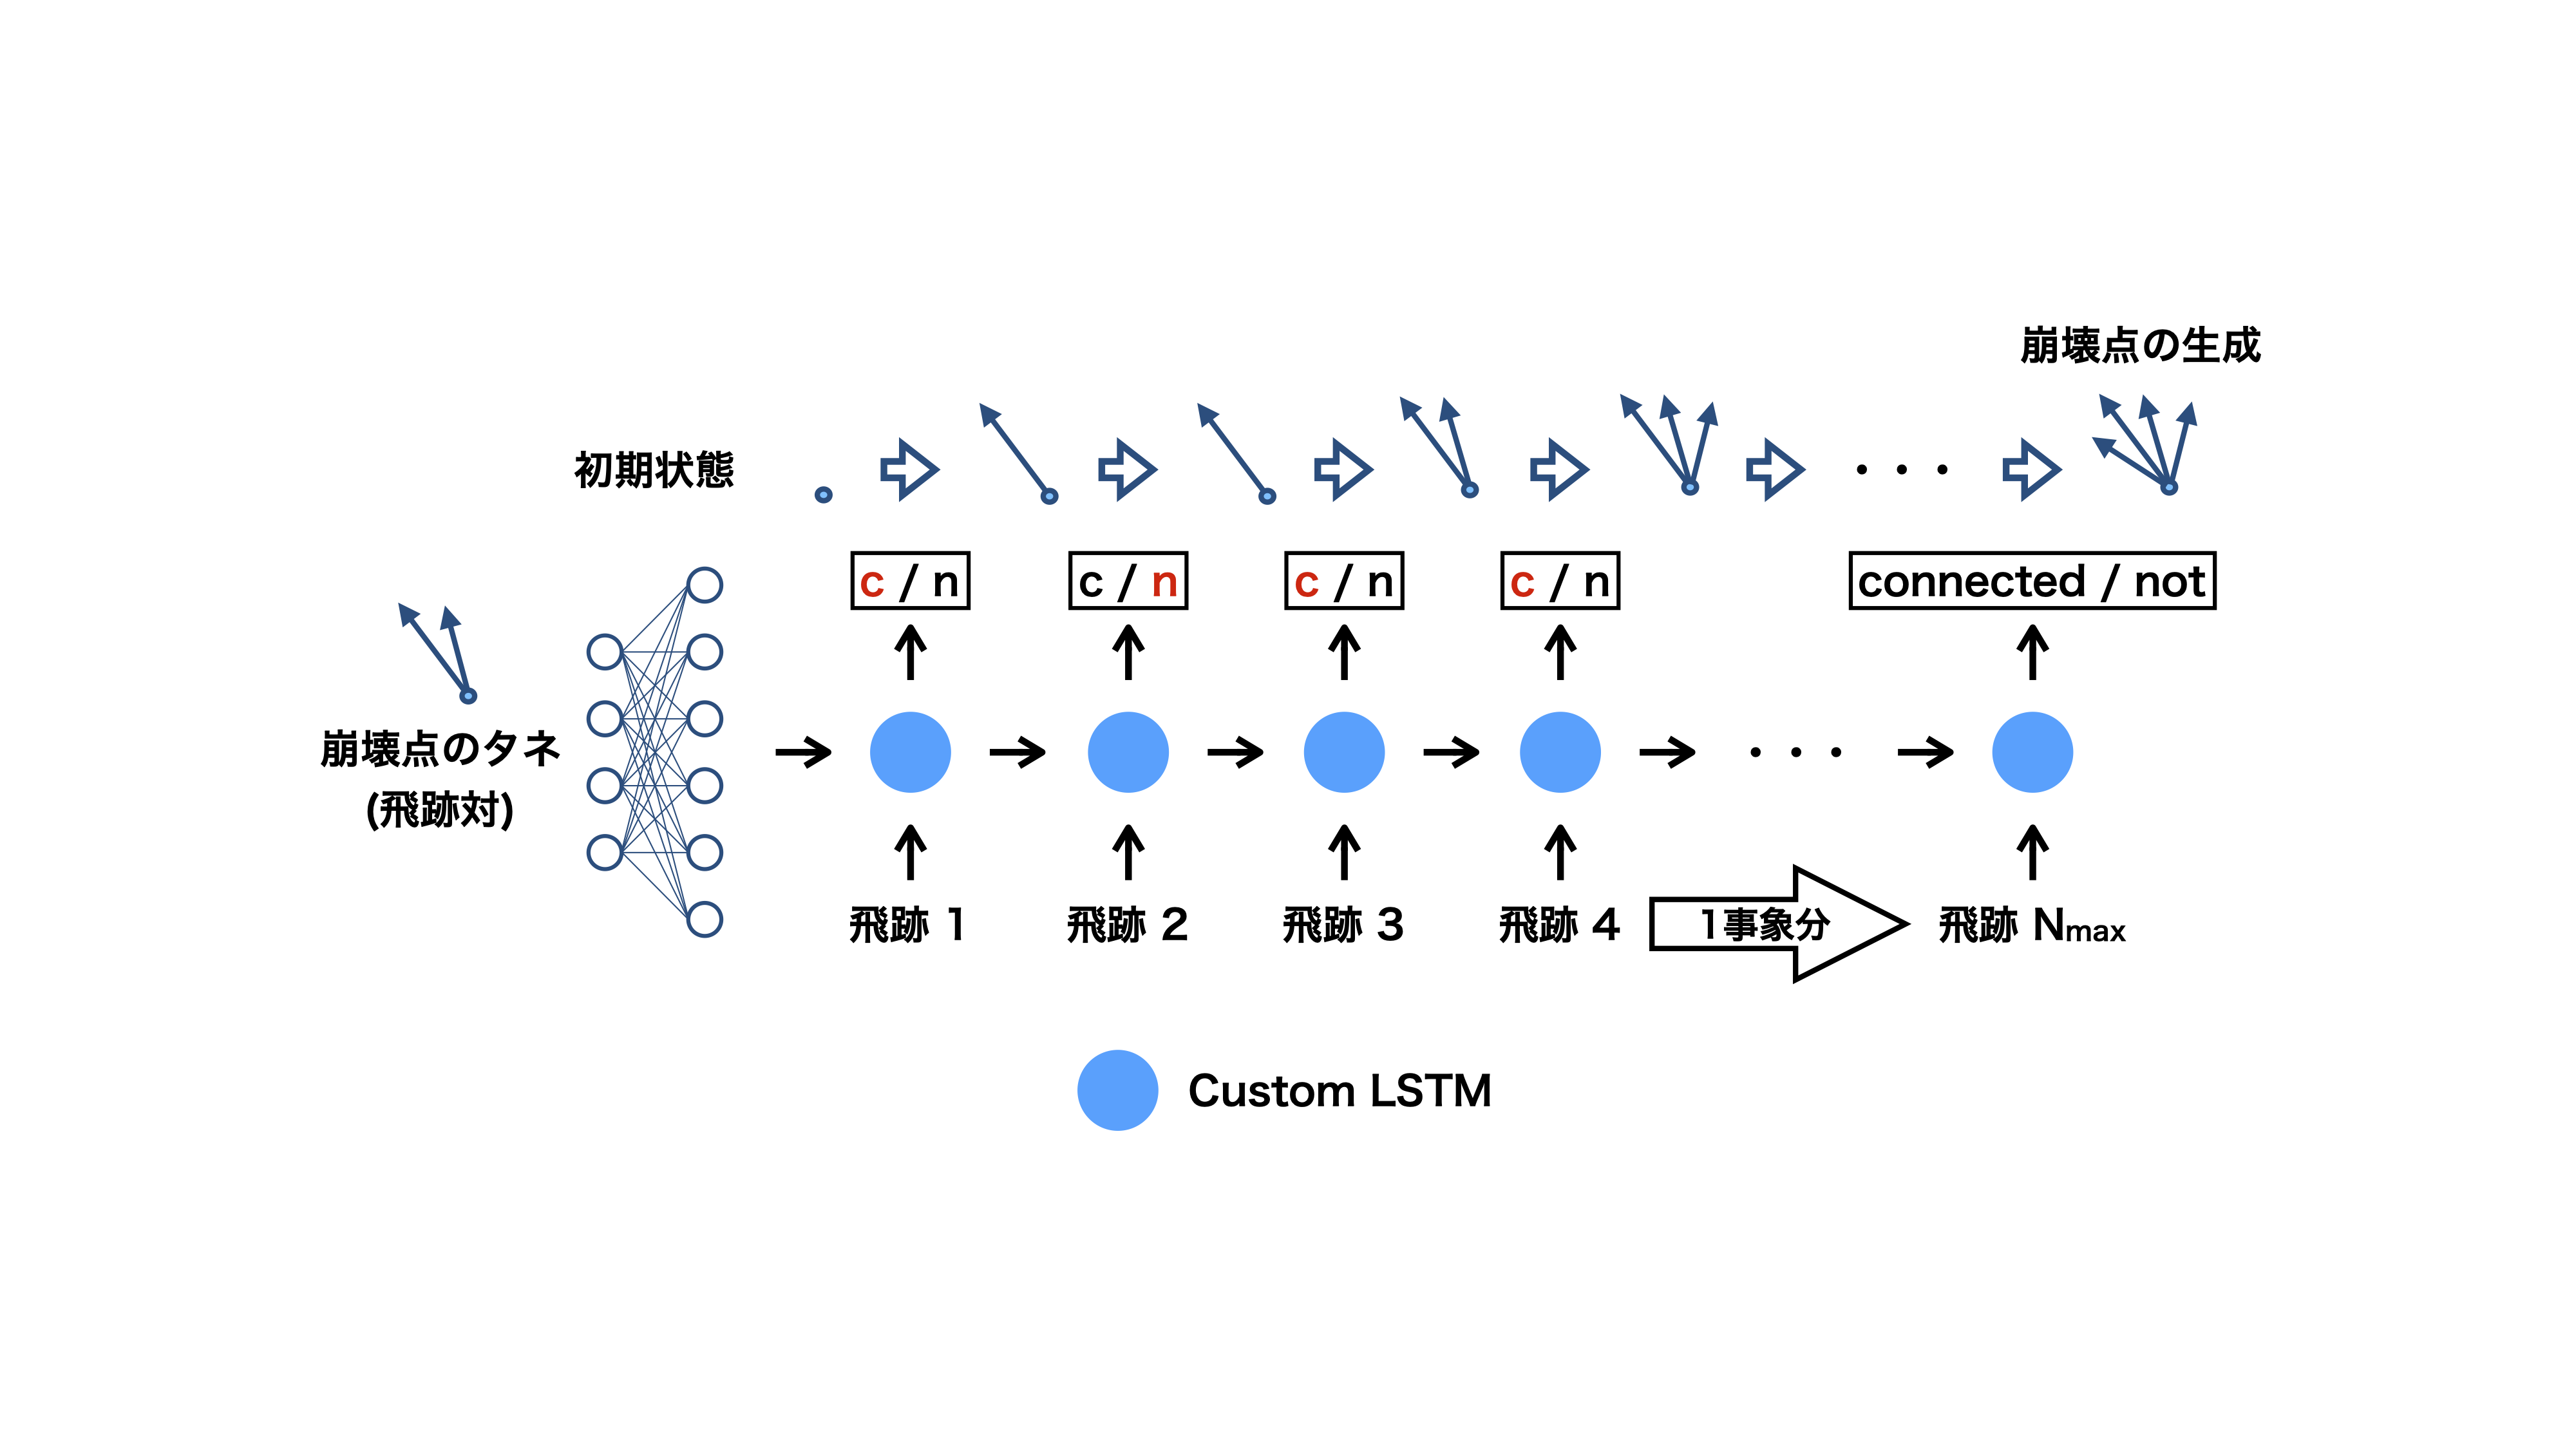
\includegraphics[trim = 0 80 0 0, width=1.0\textwidth]{Figure/3Networks/3-4-1-1SimpleVLSTM.png}
 \caption{独自のリカレントニューラルネットワーク構造を用いた崩壊点の生成}
 \label{3-4-1-1SimpleVLSTM}
\end{figure}

自然な発想として、今、飛跡について1事象分 (系列) の全ての情報を持っている為、エンコーダー・デコーダーモデルとすることで、その事象についての情報 (コンテキスト) を活用することができる。
更に、エンコーダー・デコーダーモデルの間にAttentionを組み込むことも同様に自然な発想である。
その様なネットワークを図\ref{3-4-1-2EncoderDecoderVLSTM}に示す。
この図では上から飛跡が入力されており、崩壊点の種である飛跡対は上部左右と左下から入力されている。
上部がエンコーダー部、下部がデコーダ部である。
個々の基本的な構造は図\ref{3-4-1-1SimpleVLSTM}と同一であるが、エンコーダー部には双方向リカレントニューラルネットワークを採用している。
また、デコーダー部では独自のリカレントニューラルネットワークの構造を更に拡張し、エンコーダー部の出力を初期状態の一つとしてAttentionに対応させたネットワークを使用している。
詳細は次項\ref{Net:VLSTM:DetailedStructureofVLSTM}にて述べる。

Attentionを組み込むことによって、デコーダー部の"ある"飛跡はエンコーダー部によって抽出された飛跡の情報に任意の注意を払って、1事象分の情報を取得することになる。
エンコーダー・デコーダーモデルに拡張しても、このネットワークの基本構造がリカレントニューラルネットワークであることに変わりがない為、デコーダー部の飛跡の本数を任意に変えることが可能である。

\begin{figure}[htbp]
 \centering
 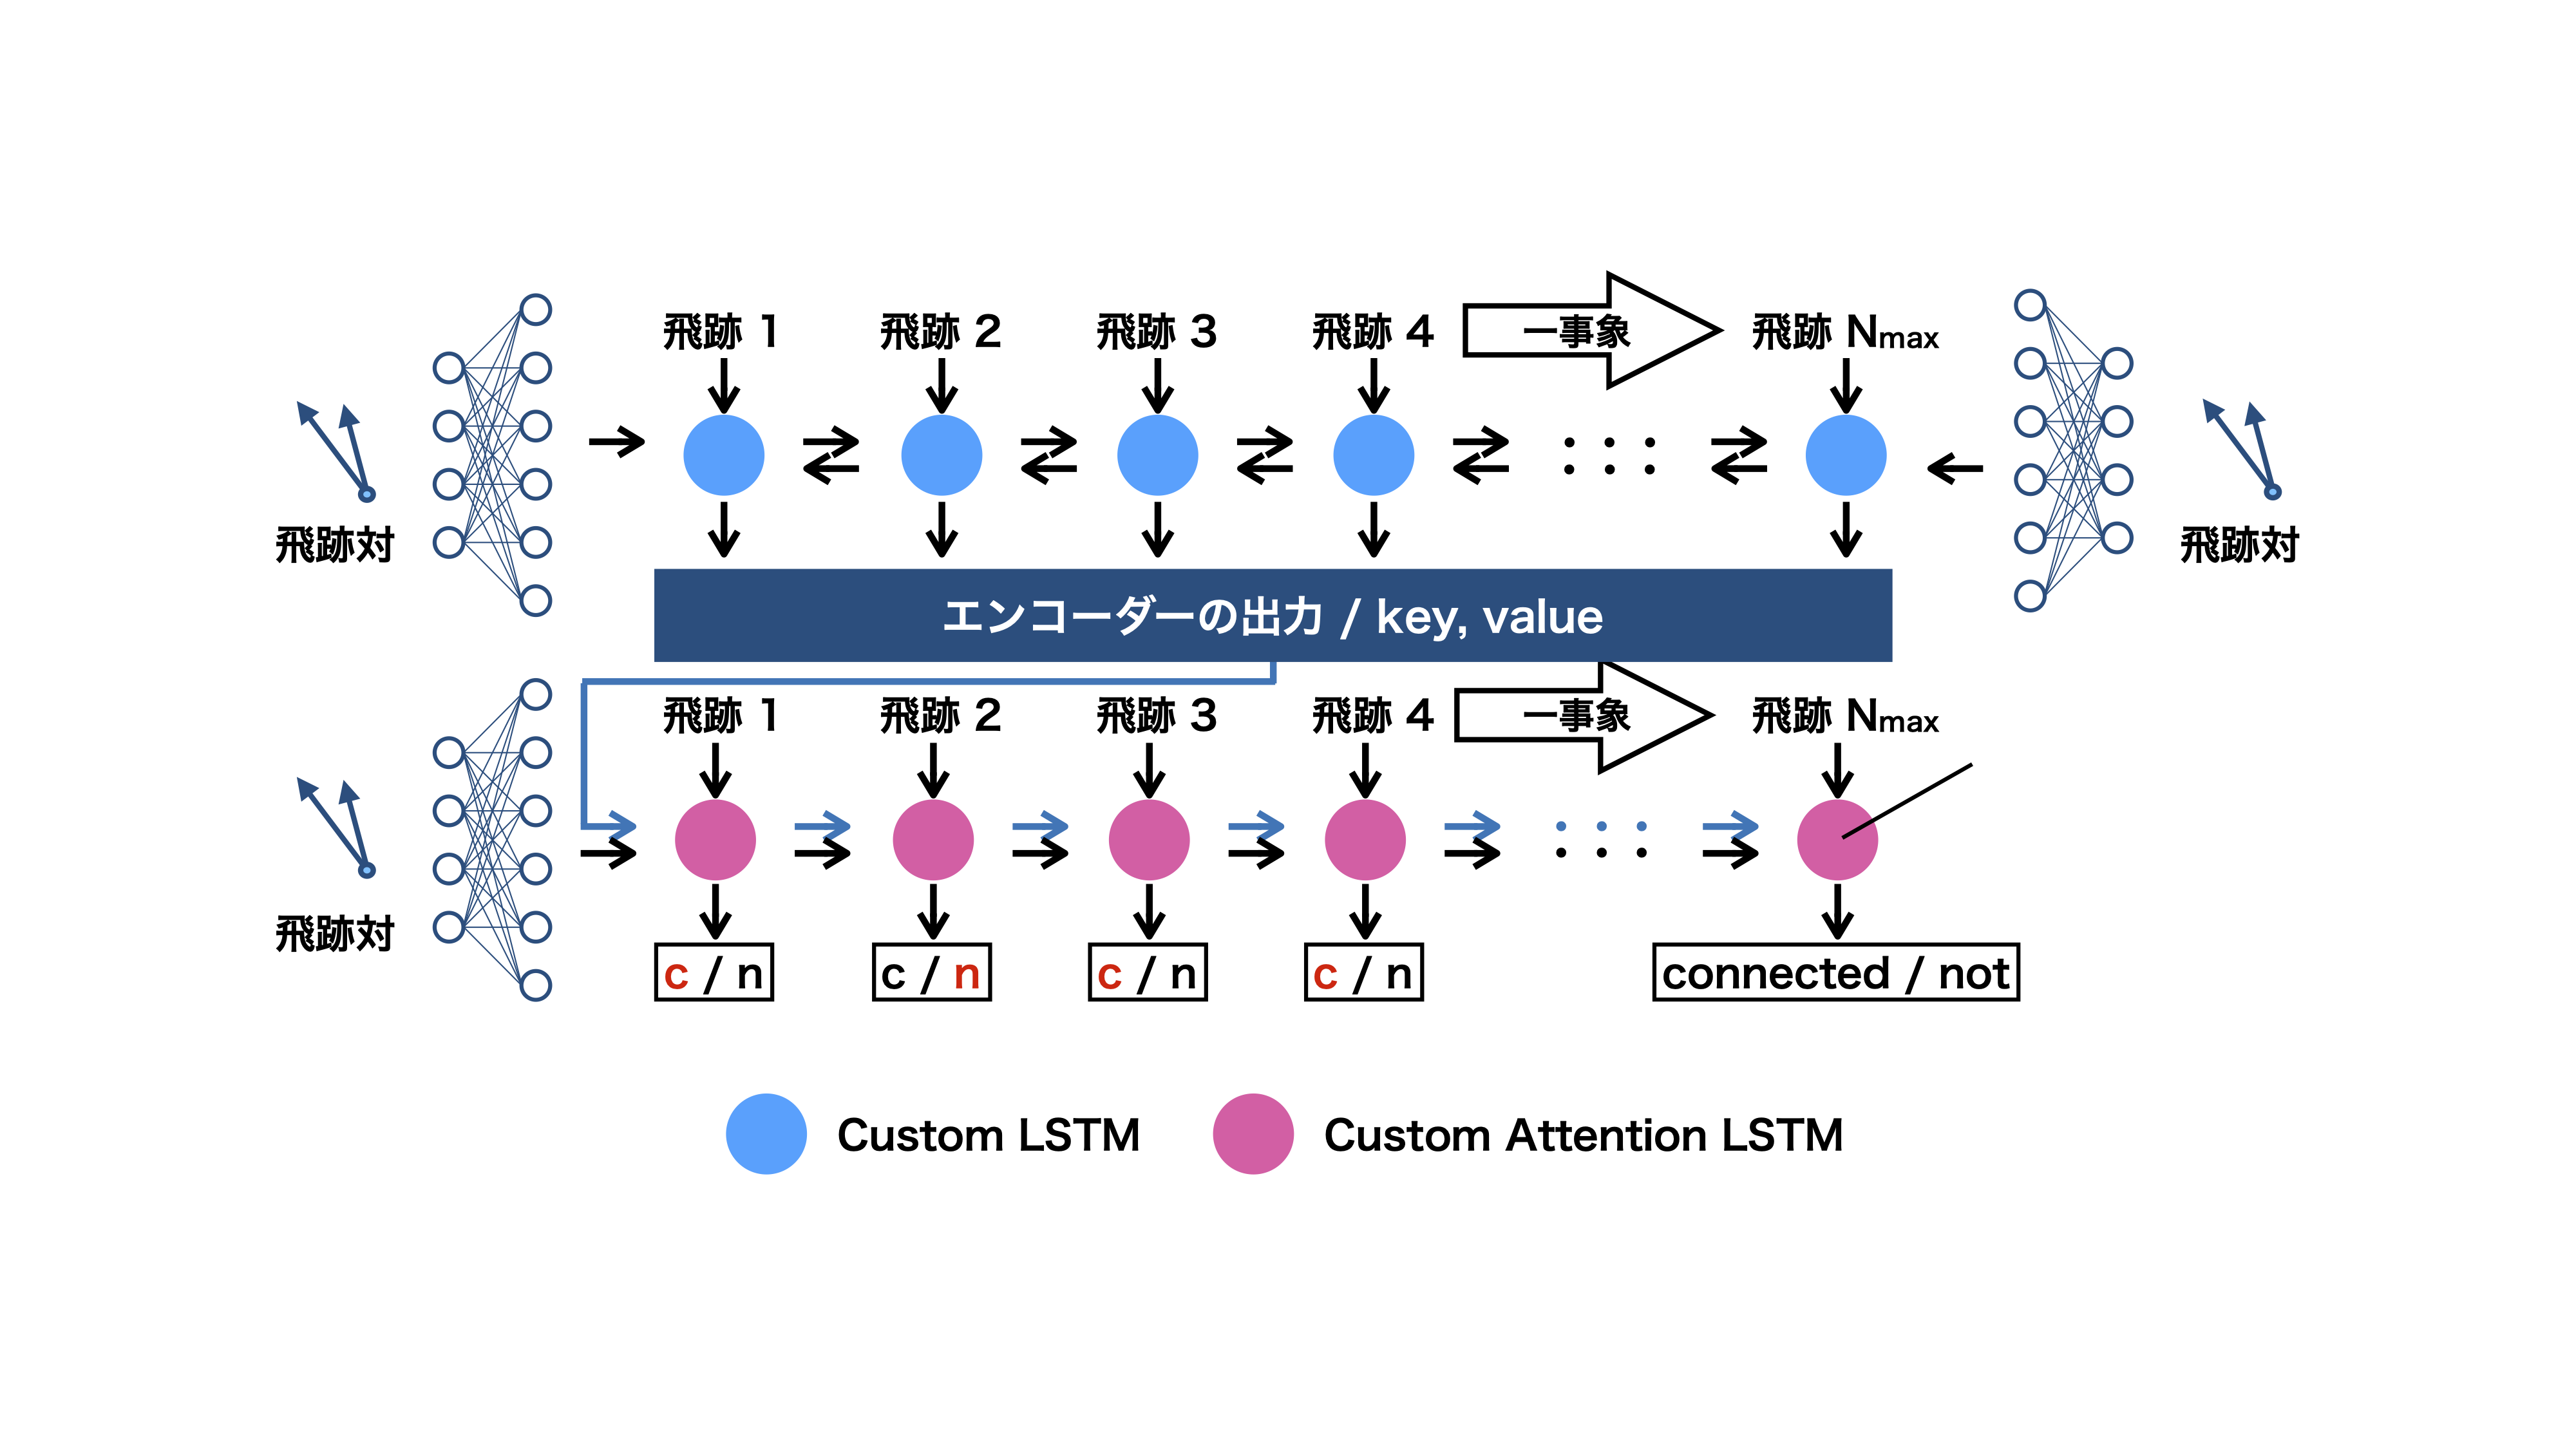
\includegraphics[trim = 0 80 0 0, width=1.0\textwidth]{Figure/3Networks/3-4-1-2EncoderDecoderVLSTM.png}
 \caption{Attentionを用いたエンコーダー・デコーダーモデルへの拡張}
 \label{3-4-1-2EncoderDecoderVLSTM}
\end{figure}

%%%%%%%%%%%%%%%%%%%%%%%%%%%%%%%%%%%%%%%%%%%%%%%%%%%%%%%%%%%%%%%%%%%%%%%%
\subsection{ネットワークの詳細な構造} \label{Net:VLSTM:DetailedStructureofVLSTM}

より詳細な構造として、ここではリカレントニューラルネットワークの1ステップを解説する。
\ref{DL:RNN:LongShortTermMemory}項では、4つのゲートと1つの記憶セルをもつLSTMを紹介した。
実際にはLSTMは短期記憶として、リカレントニューラルネットワークと同様の隠れ状態を持っていた。
この短期記憶は直前の系列についての情報を非常に多く含んでおり、本研究で使用する飛跡についてのデータの性質と合っていない。
したがって、LSTMをそのまま用いることは適切ではなく、データの性質に沿って拡張する必要がある。

このことから私は以下の図\ref{3-4-2-1VLSTMStructure}ようなネットワークを提案する。
図からも分かるようにLSTMでの短期記憶${\mbox{\boldmath{$h$}}}_t$が隠れ状態として入出力されていない。
入力は${\mbox{\boldmath{$c$}}}_{t-1},{\mbox{\boldmath{$x$}}}_t$の二つである。
ここで、${\mbox{\boldmath{$c$}}}_{t-1}$は記憶セルとしての役割を持っており、${\mbox{\boldmath{$x$}}}_t$は系列データである。
${\mbox{\boldmath{$h$}}}_t$は単に出力として使用され、${\mbox{\boldmath{$c$}}}_{t}$が隠れ状態の記憶セルとして次のステップに使用されている。
隠れ状態として${\mbox{\boldmath{$h$}}}_t$が使用されていないため、内部の構造も通常のLSTMとは少し異なり、${\mbox{\boldmath{$h$}}}_{t},\  {\mbox{\boldmath{$c$}}}_{t}$は
\begin{equation}
 \begin{split}
  {\mbox{\boldmath{$c$}}}_{t} 
  &= (1-{\mbox{\boldmath{$h$}}}_t) {\mbox{\boldmath{$c$}}}_{t-1} + {\mbox{\boldmath{$h$}}}_t {\mbox{\boldmath{$c'$}}}_{t}\\
  {\mbox{\boldmath{$c'$}}}_{t}
  &= {\mbox{\boldmath{$c$}}}_{t-1} \  \sigma (W_f {\mbox{\boldmath{$x$}}}_t + R_f {\mbox{\boldmath{$c$}}}_{t-1}) 
  + \tanh (W_c {\mbox{\boldmath{$x$}}}_t + R_c {\mbox{\boldmath{$c$}}}_{t-1}) \  \sigma (W_i {\mbox{\boldmath{$x$}}}_t + R_i {\mbox{\boldmath{$c$}}}_{t-1})\\
  {\mbox{\boldmath{$h$}}}_{t} 
  &= \sigma (D_h [\tanh({\mbox{\boldmath{$c$}}}_{t-1}) \  \sigma (W_o {\mbox{\boldmath{$x$}}}_t + R_o {\mbox{\boldmath{$c$}}}_{t-1}) ])
 \end{split}
\end{equation}
となる。
第二式の${\mbox{\boldmath{$c'$}}}_{t}$は更新された記憶セルを示している。
第一式では、更新された記憶セル${\mbox{\boldmath{$c'$}}}_{t}$と直前の系列での記憶セル${\mbox{\boldmath{$c'$}}}_{t-1}$、出力${\mbox{\boldmath{$h$}}}_{t}$を用いて現系列での記憶セル${\mbox{\boldmath{$c$}}}_{t}$を計算している。
本研究において、出力${\mbox{\boldmath{$h$}}}_{t}$は、ある崩壊点の種に対して、結合しているか否かの二値分類である。
したがって、第一式では出力${\mbox{\boldmath{$h$}}}_{t}$が結合 (${\mbox{\boldmath{$h$}}}_{t} \sim 1$) していれば更新された記憶セル${\mbox{\boldmath{$c'$}}}_{t}$を、出力${\mbox{\boldmath{$h$}}}_{t}$が非結合 (${\mbox{\boldmath{$h$}}}_{t} \sim 0$) であれば、直前の系列での記憶セル${\mbox{\boldmath{$c$}}}_{t-1}$を現系列での記憶セル${\mbox{\boldmath{$c$}}}_{t}$を選択していると解釈できる。
\ref{Net:VLSTM:StructureofVLSTM}項で述べたように、この隠れ状態の初期状態${\mbox{\boldmath{$c$}}}$として崩壊点の種を入力している。
したがって、記憶セル${\mbox{\boldmath{$c$}}}_{t}$が崩壊点についての位置などの情報であると解釈すると、このネットワークは崩壊点を逐次的に更新される様子を表現していると捉えることができる。
つまり、事象中の飛跡は系列データではないが、その飛跡を崩壊点の種に結合していく過程を記憶セルによって表現することで一本ずつ飛跡を結合し、最終的に崩壊点を生成することが可能である。

\begin{figure}[htbp]
 \centering
 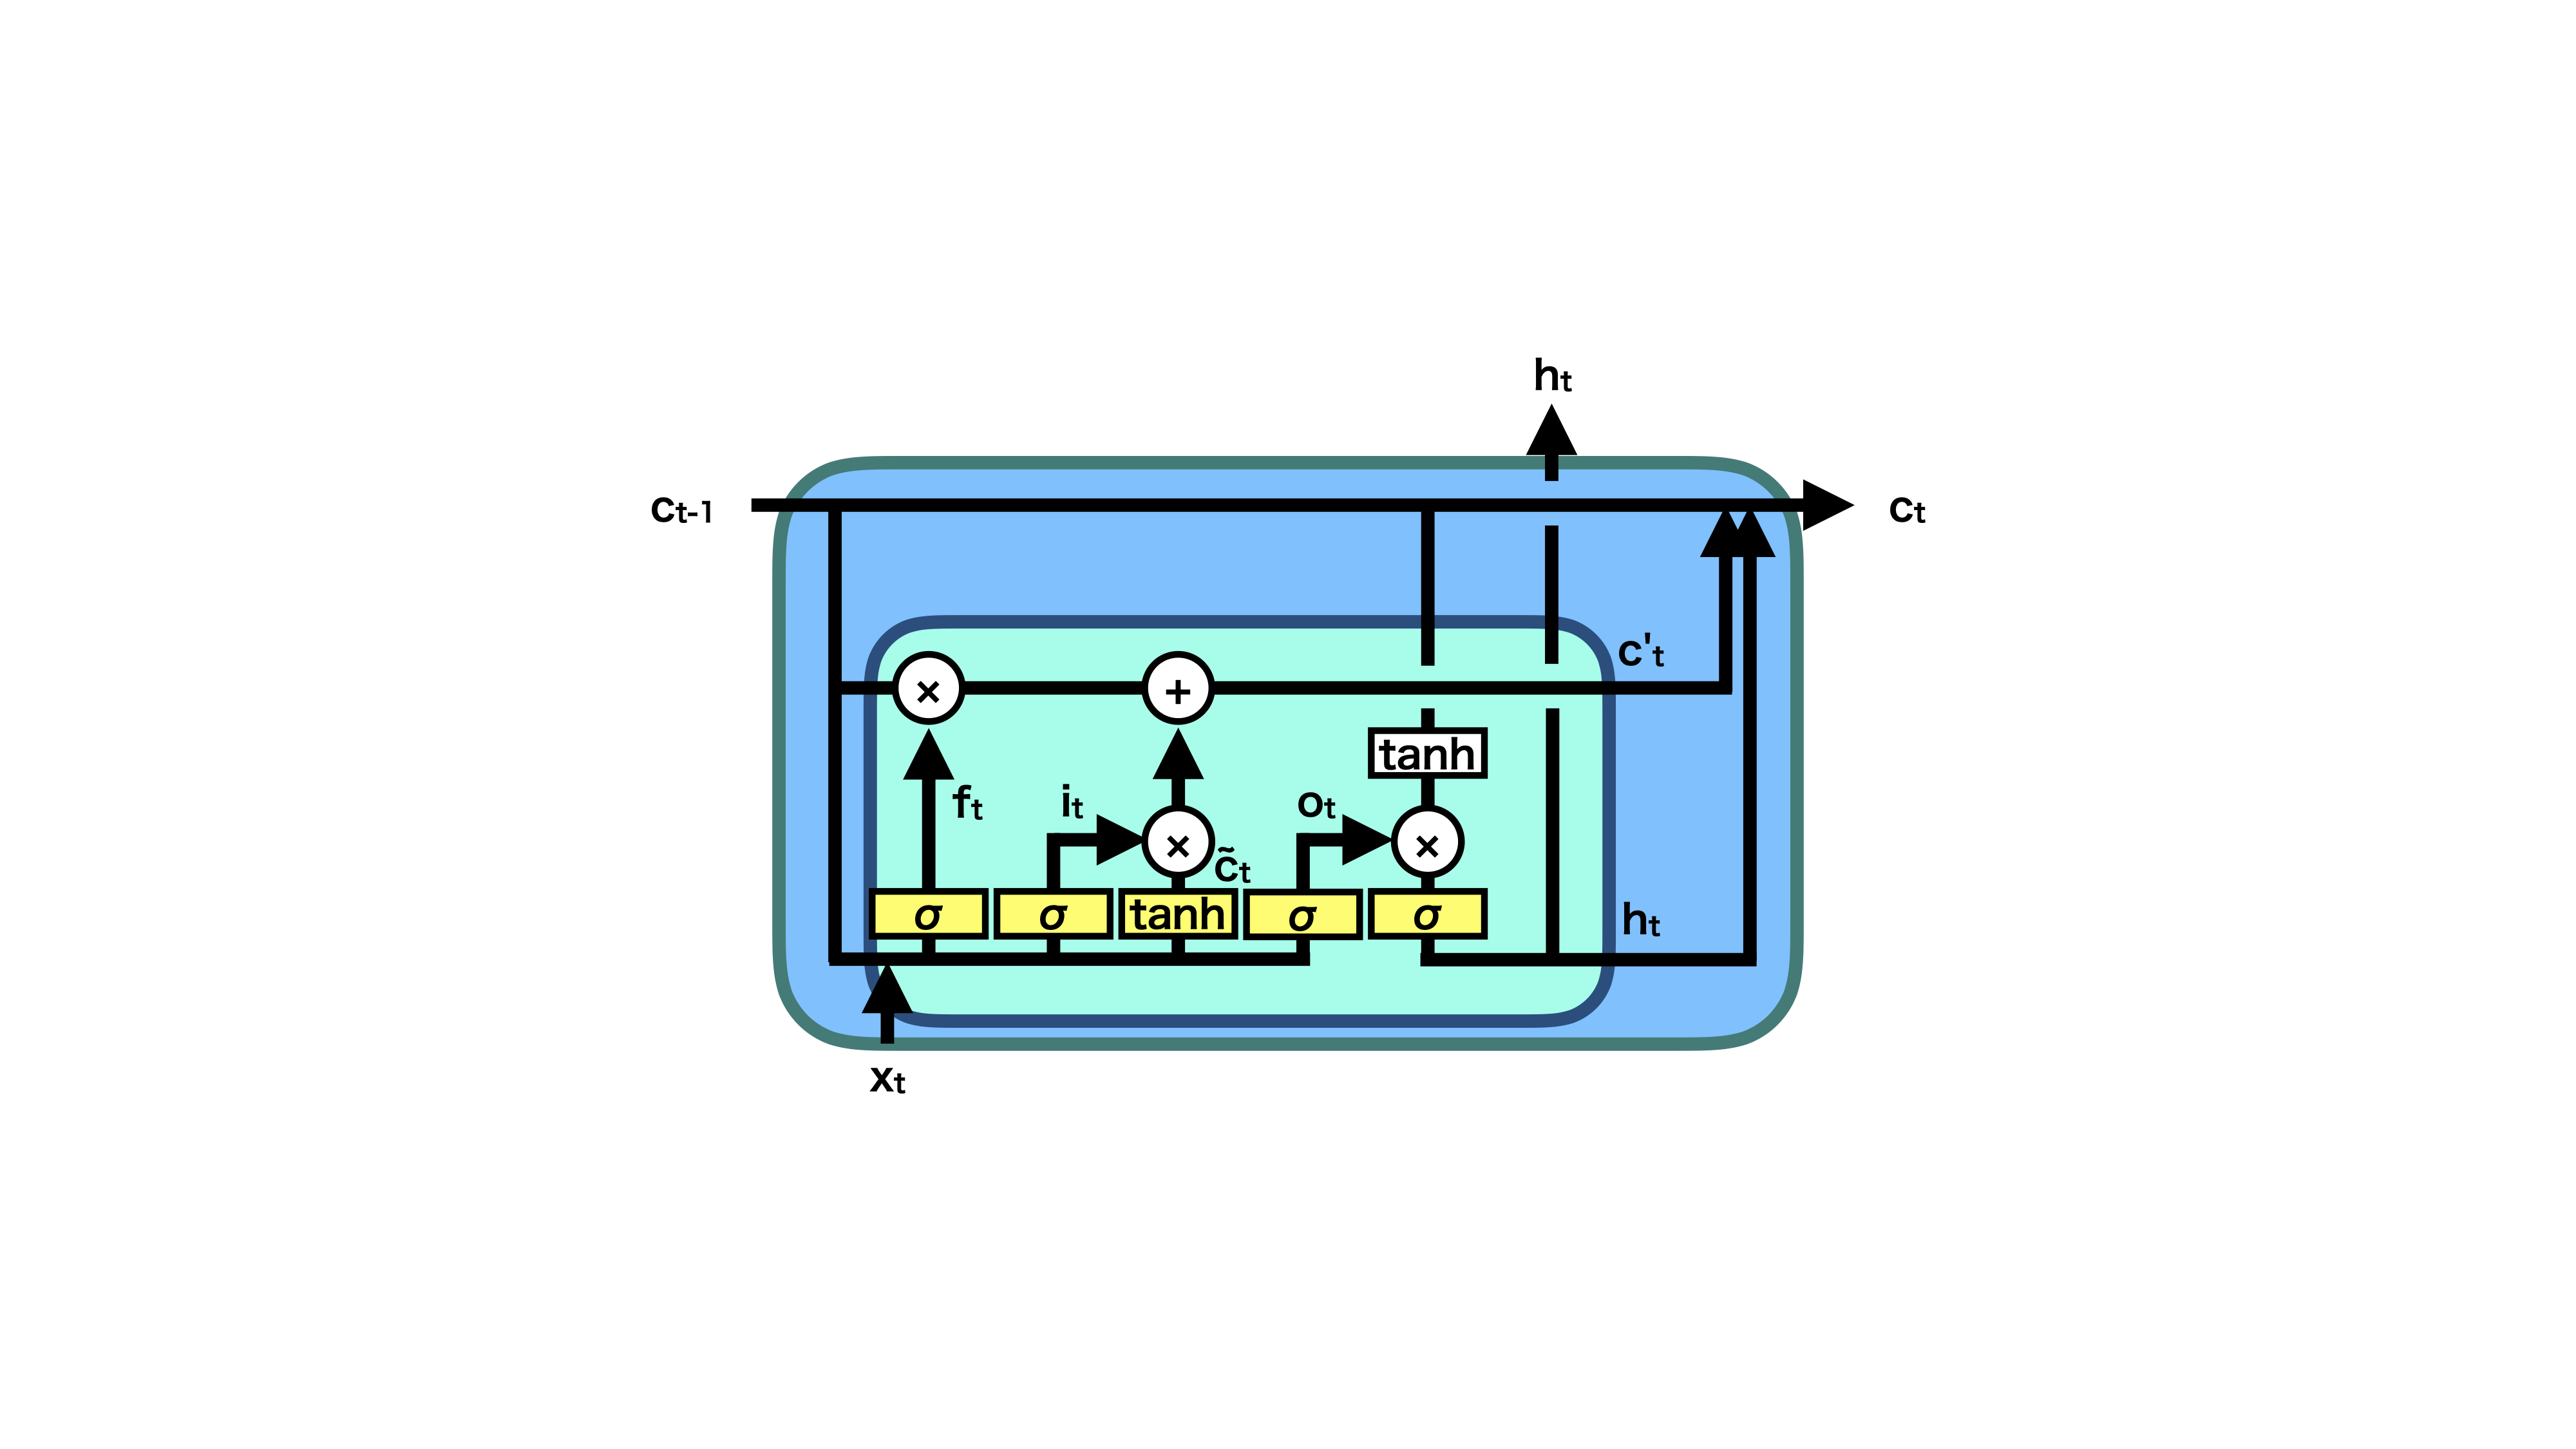
\includegraphics[trim = 200 200 200 50, width=0.9\textwidth]{Figure/3Networks/3-4-2-1VLSTMStructure.png}
 \caption{リカレントニューラルネットワークの拡張}
 \label{3-4-2-1VLSTMStructure}
\end{figure}

次にAttentionを組み込んだネットワーク構造を考える。
エンコーダー・デコーダーモデルでのエンコーダー部のネットワーク構造は図\ref{3-4-2-1VLSTMStructure}と同様のものである。
デコーダー部のネットワーク構造を図\ref{3-4-2-2AttentionVLSTM}に示す。
本研究では、Attentionに使用するkeyは隠れ状態の一つとしてネットワーク内に入力している。
また、このkeyはネットワークの各ステップについて共通のものが使用され常に同じ行列である。
ここではAttention weightの計算方法としてAdditive Attentionを選択した。
系列$t$でのAttentionによって生成されるコンテキストを${\mbox{\boldmath{$\gamma$}}}_{t}$とすると、${\mbox{\boldmath{$\gamma$}}}_{t}$は
\begin{equation}
 \begin{split}
  {\mbox{\boldmath{$\gamma$}}}_{t} 
  &= {\mbox{\boldmath{$\alpha$}}}_{t} V\\
  {\mbox{\boldmath{$\alpha$}}}_{t}
  &= (\alpha_{t,0},\ \alpha_{t,1},\ \alpha_{t,2},\ \cdots \alpha_{t,i},\ \cdots) \\
  &= \left(\frac{\exp{({{e}}_{t,0})}}{\sum_j \exp{({{e}}_{t,j})}},\ \frac{\exp{({{e}}_{t,1})}}{\sum_j \exp{({{e}}_{t,j})}},\ \frac{\exp{({{e}}_{t,2})}}{\sum_j \exp{({{e}}_{t,j})}},\  \cdots \frac{\exp{({{e}}_{t,i})}}{\sum_j \exp{({{e}}_{t,j})}},\ \cdots\right)\\
  {\mbox{\boldmath{$e$}}}_{t}
  &={\mbox{\boldmath{$u$}}}_{\rm energy} (K\ U_{\rm key} + X_t\ U_{\rm query}) \\
 \end{split}
\end{equation}
と計算される。
ここで、keyを$K$、valueを$V$、飛跡${\mbox{\boldmath{$x$}}}_{t}$を重ねた行列を$X_t$、Attention weightを${\mbox{\boldmath{$\alpha$}}}_{t}$、Attentionについてのエネルギーを${\mbox{\boldmath{$e$}}}_{t}$とした。
また、Additive Attentionにおける重み行列をそれぞれ${\mbox{\boldmath{$u$}}}_{\rm energy},\  U_{\rm key},\ U_{\rm query}$と置いた。
添字$i$はエンコーダーでの系列長だけ走る。

このようにして得られた系列$t$でのコンテキスト${\mbox{\boldmath{$\gamma$}}}_{t}$は、結合や非結合の出力や崩壊点の更新などに使用される。
\begin{equation}
 \begin{split}
  {\mbox{\boldmath{$c$}}}_{t} 
  &= (1-{\mbox{\boldmath{$h$}}}_t) {\mbox{\boldmath{$c$}}}_{t-1} + {\mbox{\boldmath{$h$}}}_t {\mbox{\boldmath{$c'$}}}_{t}\\
  {\mbox{\boldmath{$c'$}}}_{t}
  &= {\mbox{\boldmath{$c$}}}_{t-1} \  \sigma (W_f {\mbox{\boldmath{$x$}}}_t + R_f {\mbox{\boldmath{$c$}}}_{t-1} + C_f {\mbox{\boldmath{$\gamma$}}}_{t})\\
  &+ \tanh (W_c {\mbox{\boldmath{$x$}}}_t + R_c {\mbox{\boldmath{$c$}}}_{t-1} + C_c {\mbox{\boldmath{$\gamma$}}}_{t}) \  \sigma (W_i {\mbox{\boldmath{$x$}}}_t + R_i {\mbox{\boldmath{$c$}}}_{t-1} + C_i {\mbox{\boldmath{$\gamma$}}}_{t})\\
  {\mbox{\boldmath{$h$}}}_{t} 
  &= \sigma (D_h [\tanh({\mbox{\boldmath{$c$}}}_{t-1}) \  \sigma (W_o {\mbox{\boldmath{$x$}}}_t + R_o {\mbox{\boldmath{$c$}}}_{t-1} + C_o {\mbox{\boldmath{$\gamma$}}}_{t}) ])
 \end{split}
\end{equation}
コンテキスト${\mbox{\boldmath{$\gamma$}}}_{t}$に関する各ゲートの重み行列をそれぞれ$C_f,\ C_c,\ C_i,\ C_o$と置いた。
図\ref{3-4-2-2AttentionVLSTM}や式からも分かるように、Attentionに関する変更以外の基本的な計算は先ほどのネットワークと変わっていない。
したがって出力や解釈に関しては全く同じである。
またオプションとしてAttention weightを確認することで、ネットワークの内部をある程度把握することも可能である。
このAttention weightについての評価は\ref{Net:VLSTM:PerformanceofVLSTM}で行う。

\begin{figure}[htbp]
 \centering
 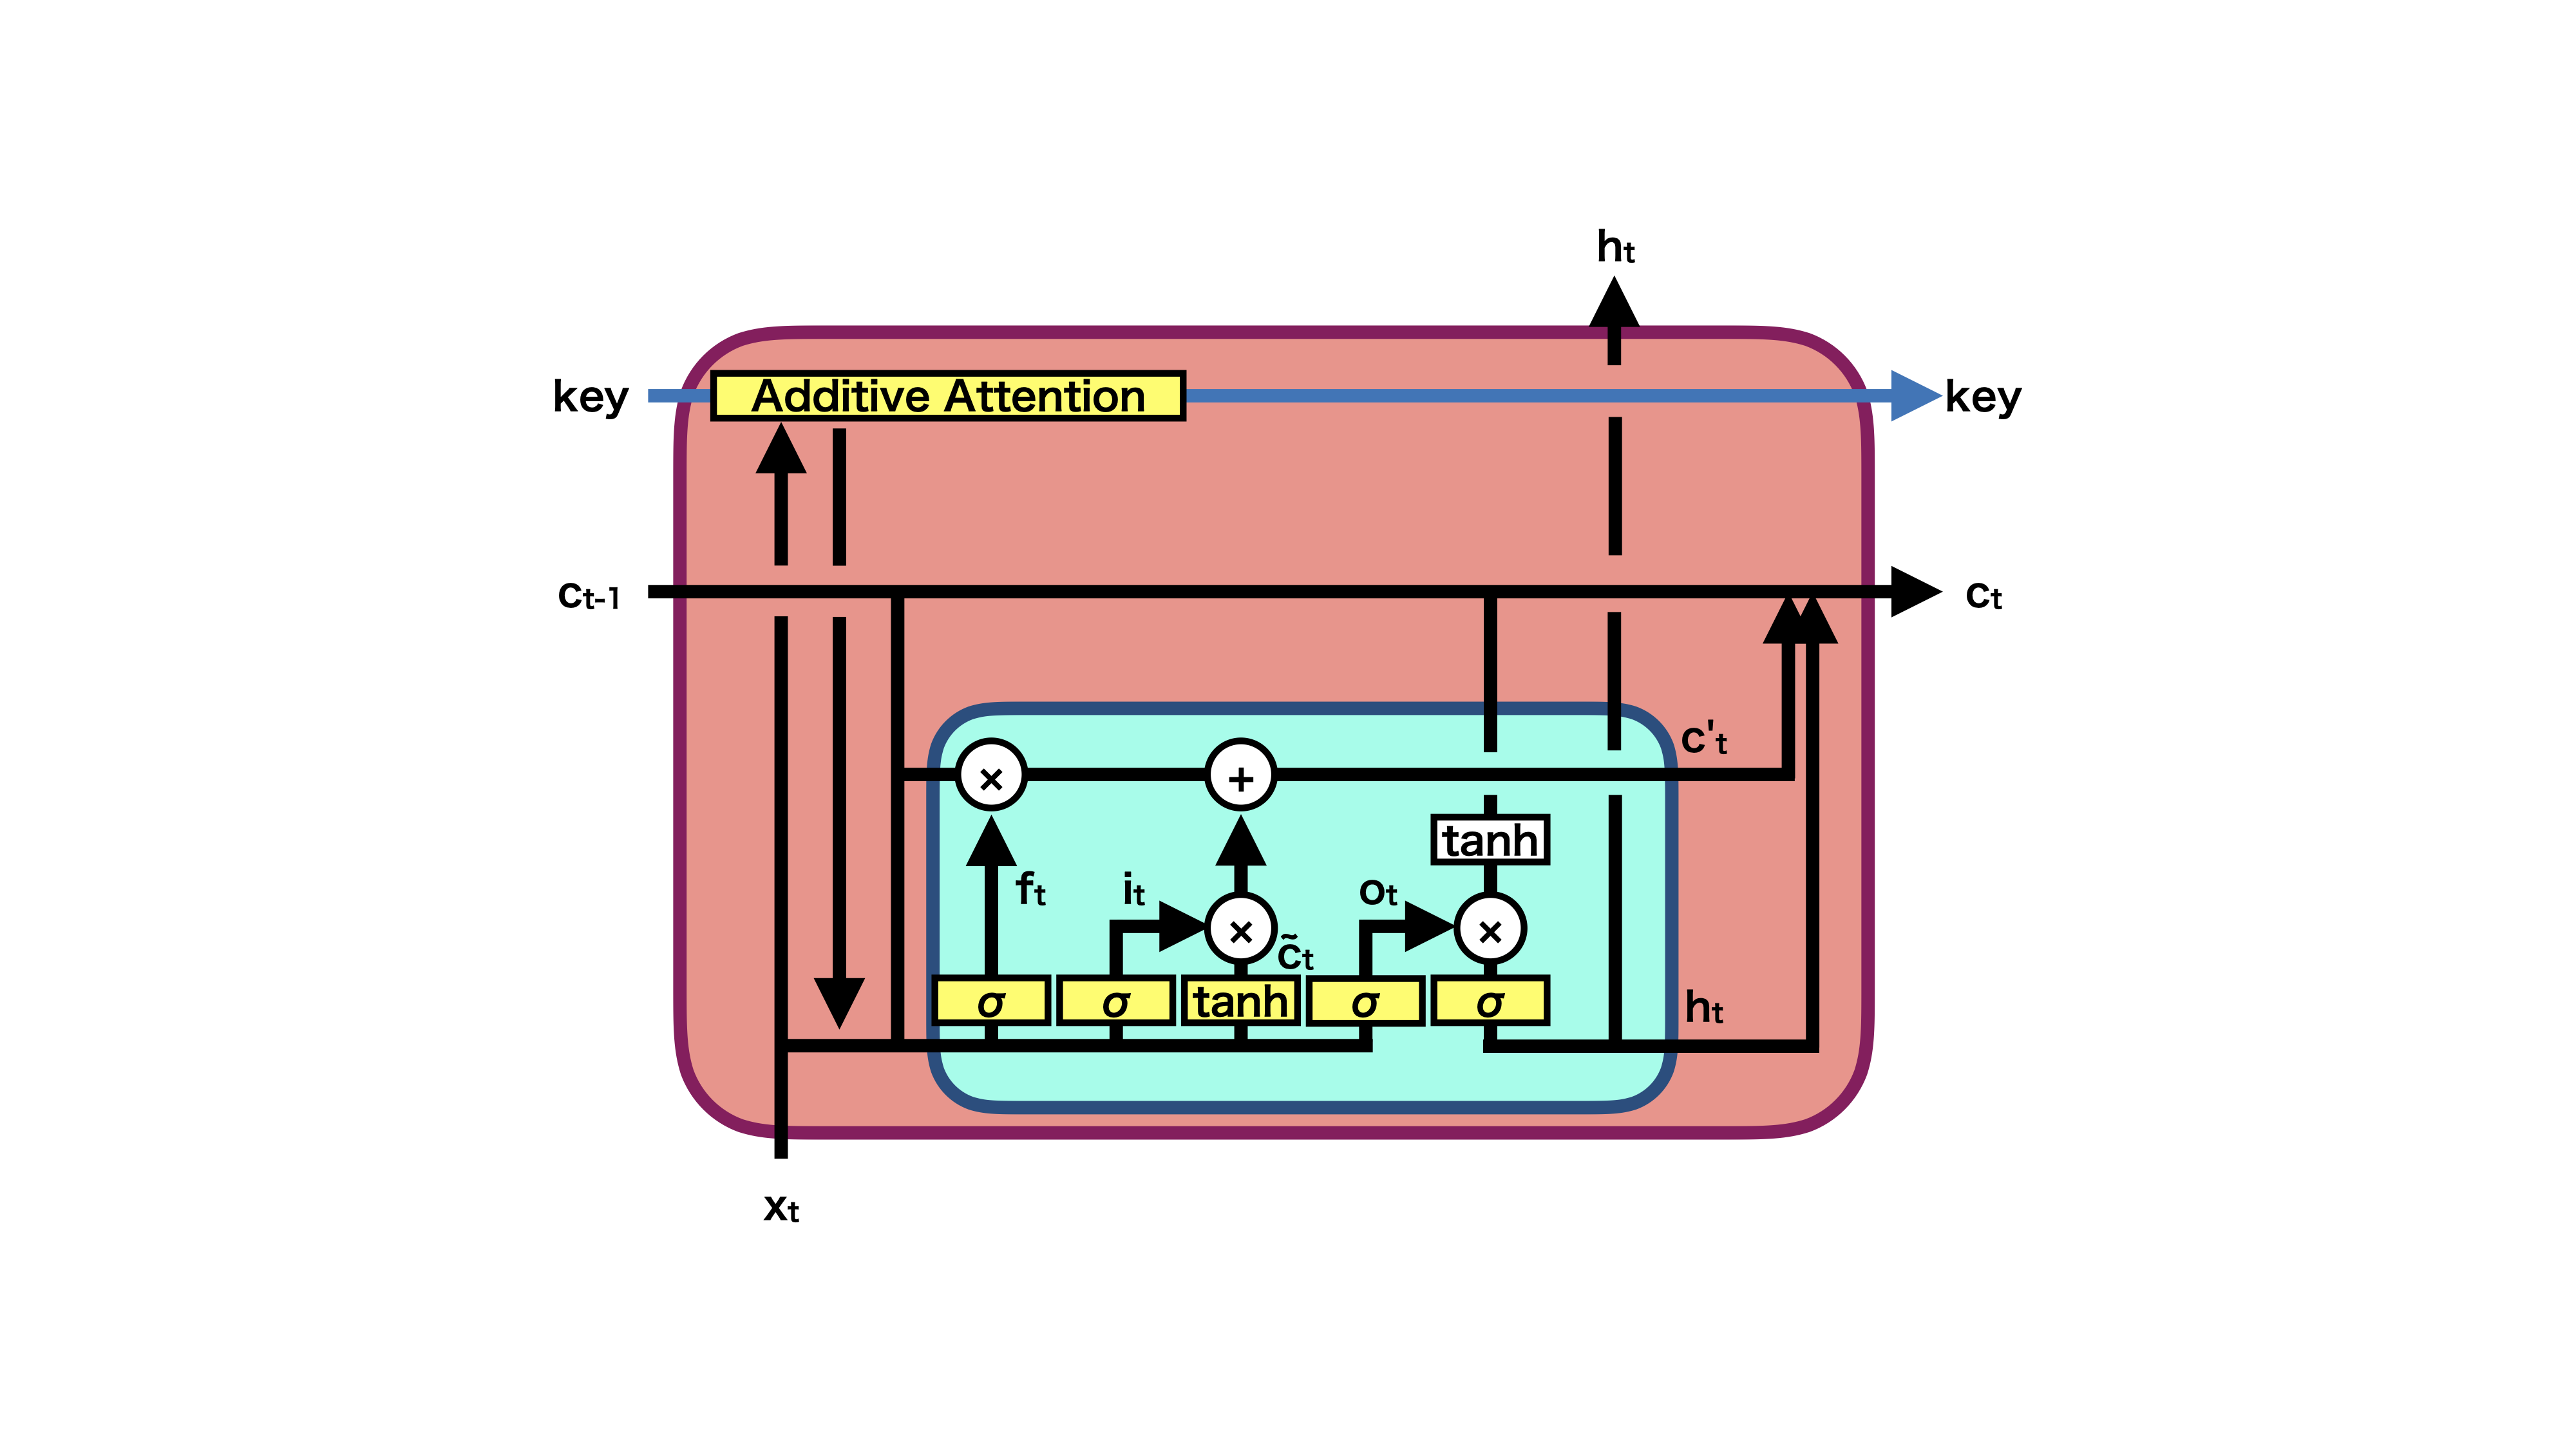
\includegraphics[trim = 100 100 100 50, width=0.9\textwidth]{Figure/3Networks/3-4-2-2AttentionVLSTM.png}
 \caption{Attentionリカレントニューラルネットワーク}
 \label{3-4-2-2AttentionVLSTM}
\end{figure}


%%%%%%%%%%%%%%%%%%%%%%%%%%%%%%%%%%%%%%%%%%%%%%%%%%%%%%%%%%%%%%%%%%%%%%%%
\subsection{ネットワークの学習と戦略} \label{Net:VLSTM:TrainingandStrategyofVLSTM}

本ネットワークの訓練データは、初期状態としての飛跡対 (崩壊点の種) と事象中の全ての飛跡、またその飛跡がそれぞれ崩壊点の種と結合しているか否かの正解ラベルである。
推論時には初期状態としての崩壊点の種には非結合な飛跡対が入力される場合が考えられるが、本研究ではネットワークの学習時は崩壊点の種は全て結合している飛跡対 (PV・SVCC・SVBB・TVCC・Others) をMCの情報を用いて選択した。
ここで、SVBCは崩壊点生成において雑音となりうる可能性があるため含んでいない。
評価での特別な場合を除いて、Primary VertexやSecondary Vertexなどの崩壊点の種類は区別していない。
またリカレントニューラルネットワークでは、推論時は系列長を変えることができるが、学習時は重み更新の計算のため系列長を揃える必要がある。
ここでの系列長は事象中の飛跡の本数である。
このため、不足している飛跡の本数をゼロ埋め (Zero padding) し、ゼロ埋めした飛跡が学習に影響しないよう損失関数をマスクしている。

崩壊点の再構成において、飛跡は順序を持って足されていく。
短期的な順序に依存しないような独自のネットワークを構築しているが、そのような人によって決められた飛跡の順序にネットワークが依存してしまうことはできる限り避けねばならないため、1エポック毎に飛跡の系列順をランダムにシャッフルしている。

\begin{figure}[htbp]
 \centering
 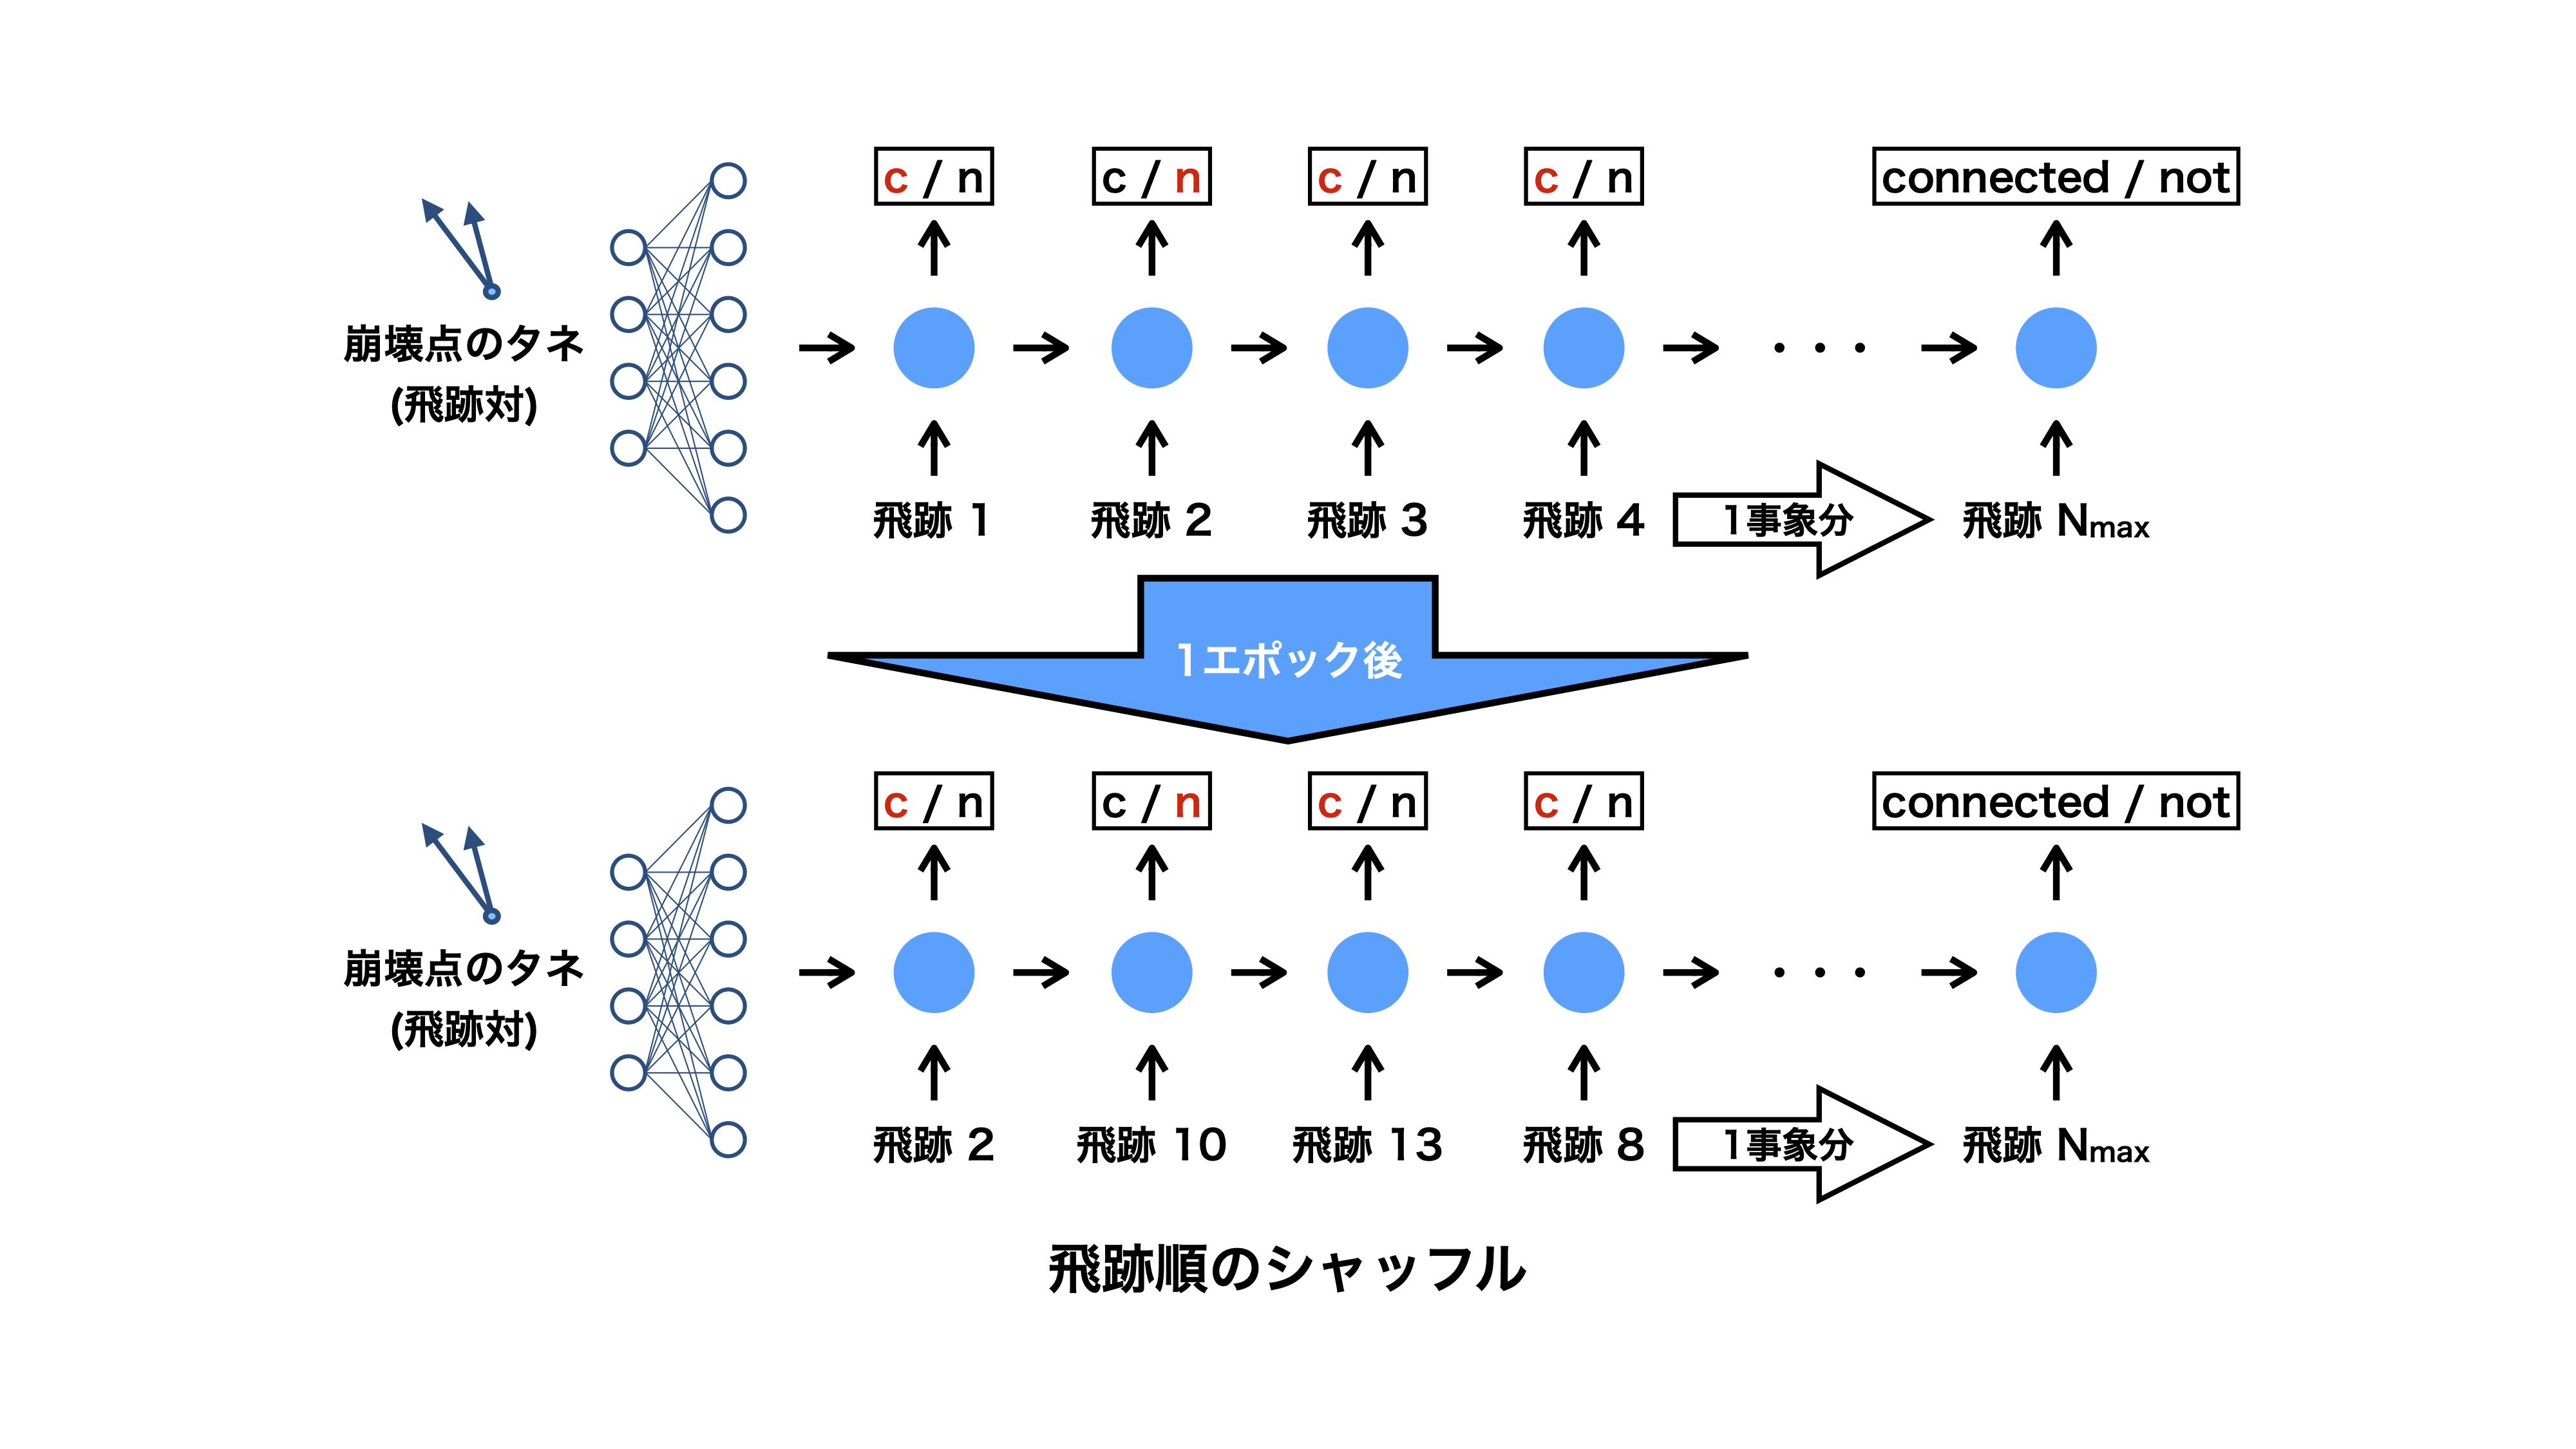
\includegraphics[width=0.9\textwidth]{Figure/3Networks/3-4-3-1TrackShuffle.png}
 \caption{飛跡順のシャッフル}
 \label{3-4-3-1TrackShuffle}
\end{figure}

訓練データは全ての崩壊点の種について一つのサンプルが生成されるため、全ての事象 ($\rm c\bar{c}-05,\ 06,\ \rm b\bar{b}-06,\ 07$) を使用すると非常に時間がかかる。
よって、本研究では全ての事象を使用して訓練データを作成した後、1エポック毎にランダムに$50000$サンプルを訓練データに$10000$サンプルを検証データに使用している。


任意の数の飛跡についてのネットワークで使用したハイパーパラメータを表\ref{HyperparametersforVLSTMModel}に示す。

\begin{table}[htb]
 \centering
 \small
  \begin{tabular}{c c}\hline
    最適化手法 & Adam\\
    学習率 & 0.001\\
    エポック数 & 100\\
    バッチサイズ & 32\\\hline
  \end{tabular}
  \caption{任意の数の飛跡についてのネットワークで使用したハイパーパラメータ}
  \label{HyperparametersforVLSTMModel}
\end{table}

損失関数は二値交差エントロピー誤差を使用した。
ただし、前述したようにゼロ埋めした飛跡については損失関数や正答率の計算ではマスクした。
また、最適化手法としてAdamを採用した。
ネットワークの詳細な構造を表\ref{ParametersforVLSTMModel}に示す。
出力の形状は (バッチサイズ, (系列長), ノード数) と表現している。
エポック数を横軸に、正答率と損失を縦軸にプロットした学習曲線を図\ref{3-4-3-2TrainingCurve}に示す。

%\begin{figure}[htbp]
 %\centering
 %\includegraphics[width=1.0\textwidth]{Figure/3Networks/3-4-3-2TrainingCurve.png}
 %\caption{任意の数の飛跡についてのネットワークの学習曲線}
 %\label{3-4-3-2TrainingCurve}
%\end{figure}


\begin{table}[htb]
 \centering
 \small
 \scalebox{0.8}{
  \begin{tabular}{l c c c}\hline
    層の名称 & 出力の形状 & パラメータ数 & 接続先\\\hline\hline
    Pair Input & (None, 44) & 0 & \\\hline
    Encoder Input & (None, 60, 23) & 0 \\\hline
    Decoder Input & (None, None, 23) & 0 \\\hline\hline
    Encoder Forward Dense 1 & (None, 256) & 11520 & Pair Input[0][0]\\\hline
    Encoder Backward Dense 1 & (None, 256) & 11520 & Pair Input[0][0]\\\hline
    Encoder Forward Activation 1 & (None, 256) & 0 & Encoder Forward Dense 1[0][0]\\\hline
    Encoder Backward Activation 1 & (None, 256) & 0 & Encoder Backward Dense 1[0][0]\\\hline
    Encoder Forward Dense 2 & (None, 256) & 11520 & Encoder Forward Activation 1[0][0]\\\hline
    Encoder Backward Dense 2 & (None, 256) & 11520 & Encoder Backward Activation 1[0][0]\\\hline
    Encoder Forward Activation 2 & (None, 256) & 0 & Encoder Forward Dense 2[0][0]\\\hline
    Encoder Backward Activation 2 & (None, 256) & 0 & Encoder Backward Dense 2[0][0]\\\hline\hline
    Encoder Embedding Dense & (None, 60, 256) & 6144 & Encoder Input[0][0]\\\hline\hline
    Bidirectional Encoder VLSTM & (None, 60, 512) & 1050624 & Encoder Embedding Dense[0][0]\\     
                                                                                                         &&&Encoder Forward Activation 2[0][0]\\       
                                                                                                         &&&Encoder Forward Activation 2[0][0]\\       
                                                                                                         &&&Encoder Backward Activation 2[0][0]\\     
                                                                                                         &&&Encoder Backward Activation 2[0][0]\\ \hline
    Reshape Bidirectional Encoder & (None, 27136) & 0 & Bidirectional Encoder VLSTM[0][0]\\\hline\hline
    Decoder Dense 1 & (None, 256) & 11520 & Pair Input[0][0]\\\hline
    Decoder Activation 1 & (None, 256) & 0 & Decoder Forward Dense 1[0][0]\\\hline
    Decoder Dense 2 & (None, 256) & 11520 & Decoder Forward Activation 1[0][0]\\\hline
    Decoder Activation 2 & (None, 256) & 0 & Decoder Forward Dense 2[0][0]\\\hline\hline
    Decoder Embedding Dense & (None, None, 256) & 6144 & Encoder Input[0][0]\\\hline\hline
    Decoder Attention VLSTM & (None, None, 1) & 1246976 & Decoder Embedding Dense[0][0]\\
                                                                                                   &&& Reshape Bidirectional Encoder[0][0]\\                    
                                                                                                   &&& Decoder Activation 2[0][0]\\\hline\hline
  \end{tabular}
  }
  \caption{任意の数の飛跡についてのネットワークにおける訓練可能なパラメータ}
  \label{ParametersforVLSTMModel}
\end{table}


%%%%%%%%%%%%%%%%%%%%%%%%%%%%%%%%%%%%%%%%%%%%%%%%%%%%%%%%%%%%%%%%%%%%%%%%
\subsection{ネットワークの性能} \label{Net:VLSTM:PerformanceofVLSTM}

コンテキストを含めて変わるか否か\\
VLSTM SimpleとEncoder-Decoderの比較 ROCカーブ\\

Attention weight\\
Connectedな飛跡を見ているか (ぬまりそうならある程度で見切りをつける)\\
PrimaryとSecondaryの差があるか\\
Attentionされている飛跡に何か傾向があるか\\

Primary, Secondary, 終状態bb, cc\\
に特化すれば性能は上がるか ROCカーブ\\









